% ========================================= TEMPLATE INFO ========================================
%
% Author:       P4ntomime
% Version:      1.0.0
% Last updated: 2024-02-18
% Brief:        A LaTeX template for summaries. See README.md for more information.
% 
% ================================================================================================
\documentclass[8pt, a4paper, twoside, landscape]{extarticle}
% Font size:    8pt
% Paper size:   A4
% style:        twoside (needed, so odd and even pages have different margins)
% orientation:  portrait. (use 'landscape' for landscape orientation)


% ========================================= DOCUMENT INFO =========================================
\def\title{Leistungselektronik}       % title
\def\shorttitle{Leistungselektronik}                            % short title (displayed as PDF title)
\def\dozent{Dr. Jasmin Smajic }               % docent
\def\semester{HS 2025}                              % semester
\def\author{Gian Marco Näf}                           % author(s)
\def\repo{https://github.com/Giamo08/Zusammenfassungen}        % repository link
\def\version{3.0.\today}                            % version
\def\pagelimit{50}                                   % page limit -> causes pages after limit to be red
\def\titleoption{ultra compact}                     % options: ultra compact, compact, normal
\def\enableToC{false}

% ================================= PACKAGES, SETUP AND COMMANDS ==================================
\input{preamble.tex}
\makeatletter
\def\@enableToC{true}
\ifx\enableToC\@enableToC
    \setcounter{tocdepth}{2} % adjust depth: 0=parts,1=sections,2=subsections,...
    \AtBeginDocument{%
        \clearpage
        \tableofcontents
        \clearpage
    }
\fi
\makeatother

% =========================================== DOCUMENT ============================================
\begin{document}
    \begin{layout}
        \section{Leistungshalbleiter in der Leistungselektronik}

\subsection{Rolle der Leistungshalbleiter im Energiesystem}

Leistungshalbleiter dienen der verlustarmen, schnellen und steuerbaren Umsetzung elektrischer Energie.
Im Gegensatz zu linearen Bauelementen arbeiten sie nicht im kontinuierlichen Arbeitsbereich,
sondern ausschliesslich als Schalter mit diskreten Zuständen.

Sie besitzen drei Betriebszustände:
\begin{itemize}
\item \textbf{leitend}: Stromfluss mit niedrigem Spannungsabfall,
\item \textbf{sperrend}: Blockieren der angelegten Spannung bis zur maximalen Sperrspannung,
\item \textbf{umschaltend}: Übergangsphase zwischen leitend und sperrend.
\end{itemize}

Damit realisieren sie:
\begin{itemize}
\item Gleichrichtung von Wechsel- zu Gleichspannung,
\item Phasenanschnitt zur Leistungssteuerung,
\item Taktbetrieb bei Gleichstromstellern (PWM),
\item Umrichtung von Spannung, Strom und Frequenz in Umrichtern.
\end{itemize}

Grundlegende Kenngrössen:
\[
U_{RRM},\quad I_{F},\quad U_F,\quad t_{on},\ t_{off},\quad P_{cond},\ P_{sw}.
\]

Dabei bezeichnet $U_{RRM}$ die maximal zulässige Sperrspannung, $I_F$ den maximalen Durchlassstrom
und $U_F$ den Spannungsabfall im leitenden Zustand.
Die Zeiten $t_{on}$ und $t_{off}$ bestimmen die Dauer der Schaltvorgänge.
$P_{cond}$ beschreibt die Leitverluste, $P_{sw}$ die Schaltverluste.

\subsection{Physikalische Grundlagen der Halbleiterbauelemente}

Alle Leistungshalbleiter beruhen auf pn-Übergängen, deren elektrisches Verhalten
durch Dotierung und Feldverteilung bestimmt wird.

Im Sperrbetrieb blockiert der pn-Übergang den Stromfluss:
\[
i \approx 0,\qquad u \le U_{RRM}
\]

Im Durchlassbetrieb ist der pn-Übergang leitend:
\[
i \gg 0,\qquad u \approx U_{on}
\]

Die maximale Sperrspannung wird bestimmt durch:
\begin{itemize}
\item die Dicke der Sperrschicht,
\item die Dotierung der Halbleiterzonen,
\item die elektrische Feldverteilung im pn-Übergang.
\end{itemize}

Thermische Belastung:
\[
\boxed{T_j = T_{amb} + R_{th} \cdot P_V}
\]

Dabei ist $T_j$ die Sperrschichttemperatur, $T_{amb}$ die Umgebungstemperatur,
$R_{th}$ der thermische Widerstand zwischen Sperrschicht und Umgebung
und $P_V$ die im Bauelement entstehende Verlustleistung.
Die Einhaltung von $T_j < T_{j,\max}$ ist zwingend für einen sicheren Betrieb.

\subsection{Diode als Leistungsschalter}

Die Leistungsdiode ist ein ungesteuertes Halbleiterbauelement mit zwei stabilen Zuständen.
Sie leitet Strom in Durchlassrichtung und blockiert in Sperrrichtung.
Sie wird vor allem in Gleichrichtern, Freilaufpfaden und als Schutzbauelement eingesetzt.

\subsubsection{Betriebszustände}

Die Leistungsdiode besitzt zwei stabile Zustände:

\textbf{Durchlass:}
\[
u_D > 0,\qquad i_D > 0
\]

\textbf{Sperre:}
\[
u_D < 0,\qquad i_D \approx 0
\]

Ideales Modell:
\[
u_D =
\begin{cases}
0, & i_D > 0 \\
\infty, & i_D = 0
\end{cases}
\]

\subsubsection{Statisches Durchlassmodell}

Reales Modell:
\[
\boxed{u_D = U_{D0} + r_D \, i_D}
\]

Hier ist $U_{D0}$ der konstante Durchlassspannungsabfall und $r_D$ der differentielle Widerstand
im leitenden Zustand.

Verlustleistung:
\[
\boxed{P_D = U_{D0} \, I_{D,\mathrm{avg}} + r_D \, I_{D,\mathrm{RMS}}^2}
\]

Dabei ist $I_{D,\mathrm{avg}}$ der Mittelwert des Diodenstroms
und $I_{D,\mathrm{RMS}}$ der Effektivwert.

Interpretation:
\begin{itemize}
\item $U_{D0}$ dominiert bei kleinen Strömen,
\item $r_D$ dominiert bei grossen Strömen.
\end{itemize}

\begin{center}
    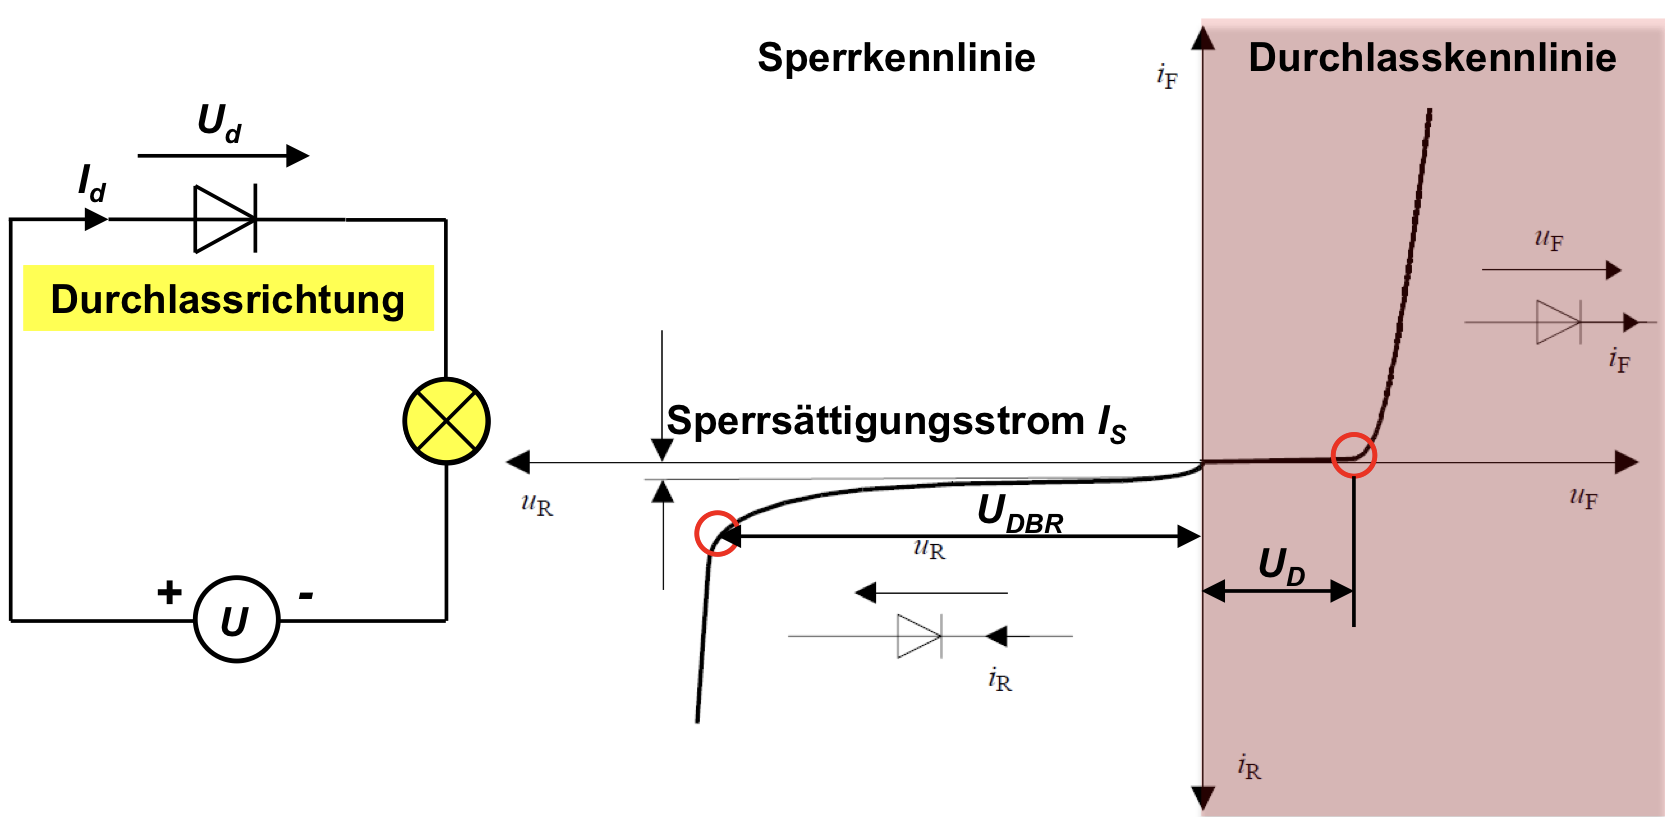
\includegraphics[width=0.85\linewidth]{images/Didodekennlinie.png}
\end{center}
\begin{center}
    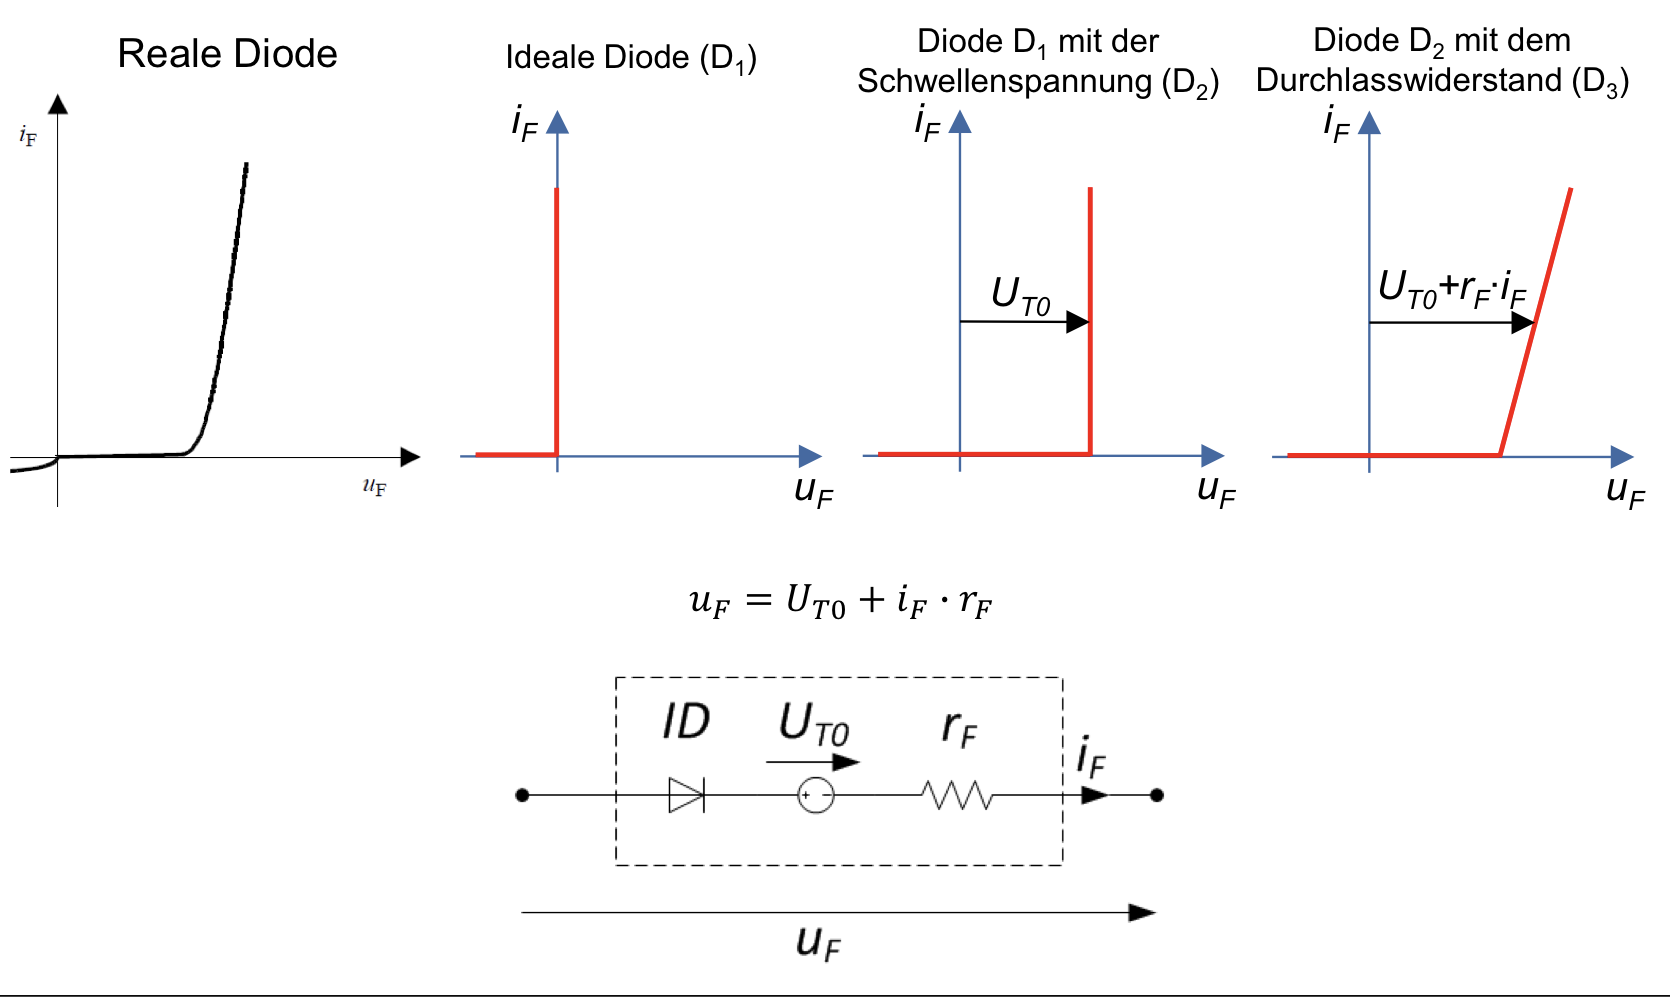
\includegraphics[width=0.85\linewidth]{images/didodeunterschied.png}
\end{center}

\subsubsection{Dynamisches Schaltverhalten}

Beim Übergang von Durchlass nach Sperre muss gespeicherte Ladung aus der Sperrschicht entfernt werden.

Rückerholstrom:
\[
i_{rr}(t)
\]

Rückerholladung:
\[
\boxed{Q_{rr} = \int_0^{t_{rr}} i_{rr}(t)\,dt}
\]

Zusätzliche Schaltverluste:
\[
\boxed{P_{sw,D} \approx f_s \, U_R \, Q_{rr}}
\]

Dabei ist $Q_{rr}$ die gespeicherte Ladung, $f_s$ die Schaltfrequenz
und $U_R$ die anliegende Sperrspannung.

Physikalische Bedeutung:
\begin{itemize}
\item grosse $Q_{rr}$ $\Rightarrow$ hohe Schaltverluste,
\item schnelle Dioden notwendig bei hohen $f_s$.
\end{itemize}

\begin{center}
    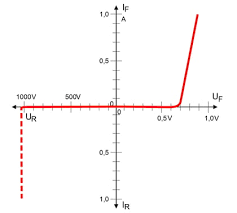
\includegraphics[width=0.85\linewidth]{images/rueckerhol.png}
\end{center}

\subsection{Thyristor (SCR)}

Der Thyristor ist ein gesteuerter, selbsthaltender Leistungsschalter mit PNPN-Struktur.
Er wird durch einen kurzen Gate-Strom gezündet und bleibt leitend,
solange der Anodenstrom oberhalb des Haltestroms liegt.
Ein aktives Abschalten ist nicht möglich.

\subsubsection{Vier-Schichten-Struktur und Zündprinzip}

Der Thyristor besitzt eine PNPN-Struktur.

Zündbedingung:
\[
u_{AK} > 0 \quad \text{und} \quad i_G > 0
\]

Nach dem Zünden:
\[
\boxed{\text{Selbsthaltung durch innere Rückkopplung}}
\]

Haltestrom:
\[
\boxed{i_A > I_H}
\]

Abschalten nur durch:
\begin{itemize}
\item Stromnulldurchgang,
\item externe Kommutierung.
\end{itemize}

\begin{center}
    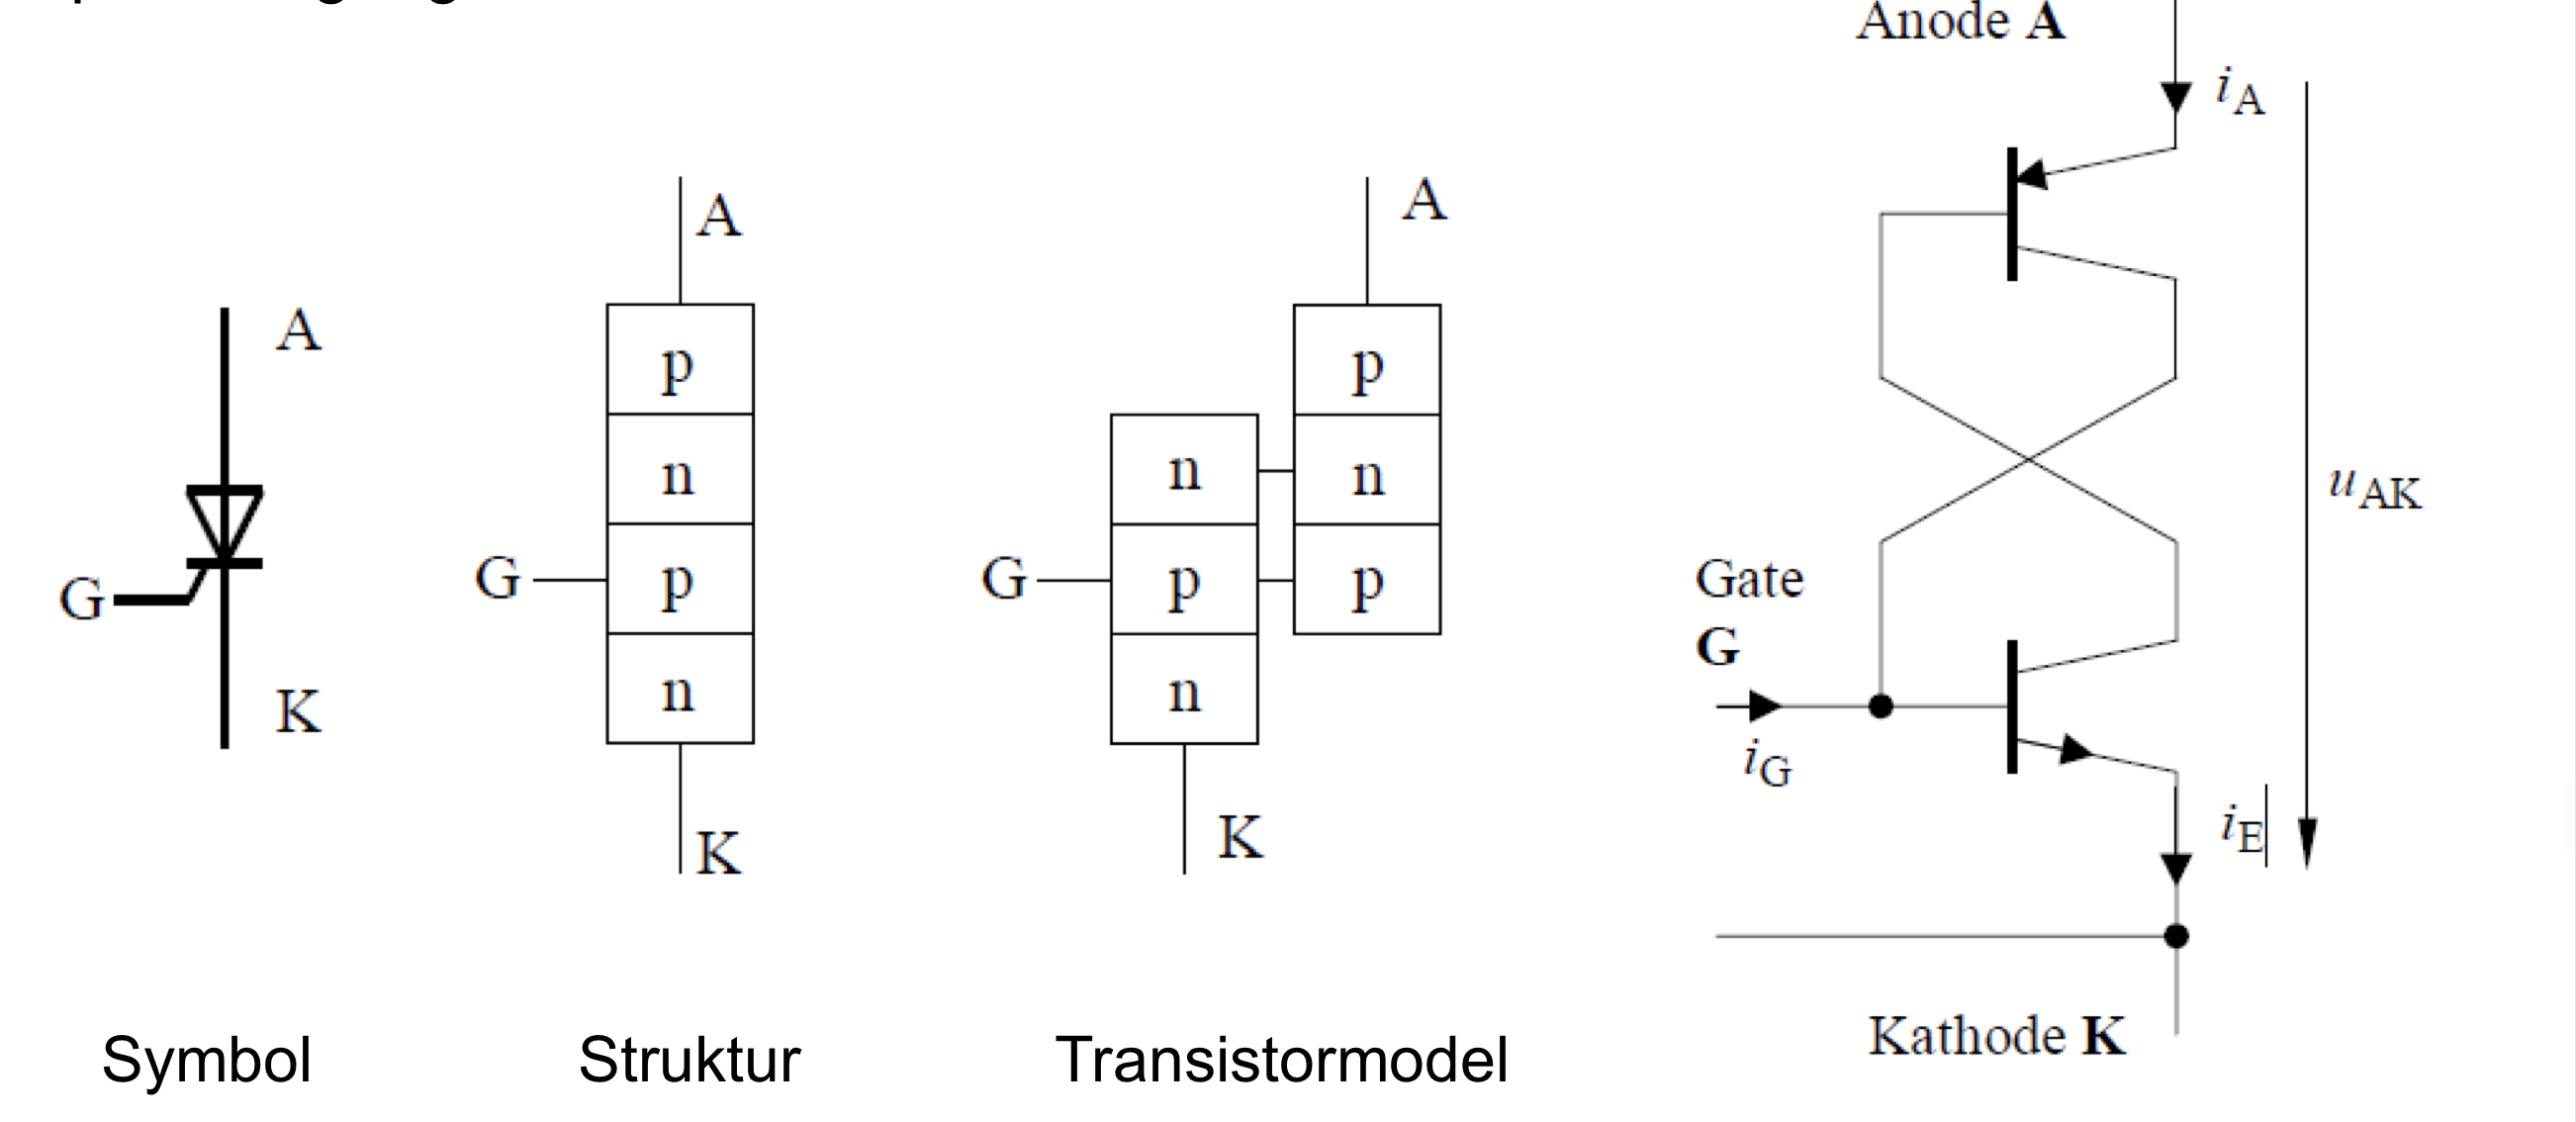
\includegraphics[width=0.85\linewidth]{images/thyristor.png}
\end{center}

\subsubsection{Statisches Modell und Verluste}

\[
\boxed{u_T = U_{T0} + r_T \, i_T}
\]

Hier ist $U_{T0}$ der konstante Durchlassabfall und $r_T$ der differentielle Widerstand.

\[
\boxed{P_T = U_{T0} \, I_{T,\mathrm{avg}} + r_T \, I_{T,\mathrm{RMS}}^2}
\]

Zusätzliche Kenngrössen:
\[
\frac{di}{dt}_{\max},\qquad \frac{du}{dt}_{\max}
\]

Diese Grenzwerte begrenzen die zulässige Strom- und Spannungssteilheit beim Zünden.

Bedeutung:
\begin{itemize}
\item Begrenzen den Zündstromanstieg,
\item Schutz durch Snubber notwendig.
\end{itemize}

\subsection{Leistungs-MOSFET}

Der Leistungs-MOSFET ist ein spannungsgesteuerter Halbleiterschalter.
Er wird über das Gate eingeschaltet und benötigt keinen Gate-Strom im stationären Zustand.
Er eignet sich besonders für hohe Schaltfrequenzen.

\subsubsection{Gate-gesteuerter Feldeffekttransistor}

Leitbedingung:
\[
\boxed{u_{GS} > U_{th}}
\]

Dabei ist $U_{th}$ die Gate-Schwellspannung.

Im leitenden Zustand:
\[
\boxed{u_{DS} = r_{DS,on} \, i_D}
\]

Charakteristisch:
\begin{itemize}
\item Mehrheitsladungsträger,
\item kein Speicherladungseffekt,
\item sehr schnelles Schalten.
\end{itemize}

\begin{center}
    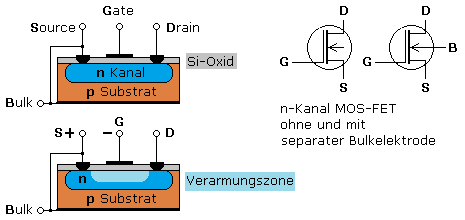
\includegraphics[width=0.85\linewidth]{images/MOSFET.png}
\end{center}

\subsubsection{Dynamisches Modell und Gate-Ladung}

Gate-Ladung:
\[
Q_G = Q_{GS} + Q_{GD}
\]

Dabei ist $Q_G$ die gesamte zum Schalten notwendige Gate-Ladung.

Schaltzeit:
\[
t_{on} \approx \frac{Q_G}{I_G}
\]

Hier bestimmt der verfügbare Gate-Strom $I_G$ die erreichbare Schaltgeschwindigkeit.

Schaltverluste:
\[
\boxed{P_{sw,M} \approx f_s \int u_{DS}(t)i_D(t)\,dt}
\]

\subsection{IGBT}

Der IGBT ist ein hybrides Bauelement aus MOS-Gate und bipolarer Stromleitung.
Er verbindet die einfache Ansteuerung des MOSFET mit den geringen Leitverlusten bipolarer Bauelemente.
Er wird vor allem bei mittleren Schaltfrequenzen und hohen Strömen eingesetzt.

\subsubsection{Hybridstruktur MOS–Bipolar}

Der IGBT kombiniert:
\begin{itemize}
\item spannungsgesteuertes MOS-Gate,
\item stromtragende bipolare Struktur.
\end{itemize}

Leitbedingung:
\[
\boxed{u_{GE} > U_{th}}
\]

Durchlassmodell:
\[
\boxed{u_{CE} = U_{CE0} + r_{CE} \, i_C}
\]

\begin{center}
    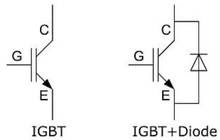
\includegraphics[width=0.85\linewidth]{images/IGBT.png}
\end{center}

\subsubsection{Tail-Strom und Abschaltverluste}

Beim Abschalten verbleibt gespeicherte Ladung im Driftgebiet.

Tail-Strom:
\[
i_{tail}(t)
\]

Zusätzliche Verluste:
\[
\boxed{P_{off} \gg P_{on}}
\]

Konsequenz:
\begin{itemize}
\item langsamer als MOSFET,
\item dafür geringere Leitverluste bei grossen Strömen.
\end{itemize}

\subsection{Vergleich der Bauelemente}

\begin{center}
\begin{tabular}{l|c|c|c|c}
 & Diode & Thyristor & MOSFET & IGBT \\
\hline
Steuerbar & nein & Zünden & ja & ja \\
Abschaltbar & ja & nein & ja & ja \\
Schaltfreq. & mittel & tief & sehr hoch & mittel \\
Leitverluste & klein & klein & klein bei klein $I$ & klein bei gross $I$ \\
Speicherladung & ja & ja & nein & ja \\
\end{tabular}
\end{center}

\subsection{Safe Operating Area (SOA)}

Die Safe Operating Area beschreibt den zulässigen Arbeitsbereich eines Leistungshalbleiters
im Strom--Spannungs--Diagramm.

Zulässige Grenzbedingungen:
\[
\boxed{
\begin{aligned}
u &< U_{RRM} \\
i &< I_{\max} \\
P &= u \cdot i < P_{\max} \\
\frac{di}{dt} &< \left(\frac{di}{dt}\right)_{\max} \\
\frac{du}{dt} &< \left(\frac{du}{dt}\right)_{\max}
\end{aligned}
}
\]

Physikalische Bedeutung:
\begin{itemize}
\item Begrenzung durch Durchbruchspannung,
\item Begrenzung durch thermische Überlast,
\item Begrenzung durch sekundären Durchbruch.
\end{itemize}

Die Einhaltung der SOA ist zwingend für den sicheren Betrieb.

\subsection{Zusammenfassung der Verlustmechanismen}

Gesamtverluste:
\[
\boxed{P_V = P_{cond} + P_{sw}}
\]

Dabei beschreibt $P_{cond}$ die Verluste im leitenden Zustand
und $P_{sw}$ die Verluste während der Schaltvorgänge.

\[
P_{cond} = U_0 I_{\mathrm{avg}} + r I_{\mathrm{RMS}}^2
\]
\[
P_{sw} = f_s \int u(t)i(t)\,dt
\]

Thermische Auslegung:
\[
T_j = T_{amb} + R_{th} P_V < T_{j,\max}.
\]

\subsection{Vereinfachte Schaltverlustrechnung}

Bei näherungsweise linearem Spannungs- und Stromverlauf während des Schaltens gilt:

\paragraph{Einschaltverlust}

\[
\boxed{E_{on} \approx \frac{1}{2} U \, I \, t_{on}}
\]

\paragraph{Ausschaltverlust}

\[
\boxed{E_{off} \approx \frac{1}{2} U \, I \, t_{off}}
\]

Mittlere Schaltverluste:

\[
\boxed{
P_{sw} = f_s \left(E_{on} + E_{off}\right)
}
\]

Konsequenzen:
\begin{itemize}
\item $f_s \uparrow \Rightarrow P_{sw} \uparrow$
\item $t_{on}, t_{off}$ klein $\Rightarrow$ geringe Verluste.
\end{itemize}

\subsection{Thermische Widerstandskette}

\[
\boxed{R_{th,tot} = R_{th,jc} + R_{th,ck} + R_{th,ka}}
\]

Temperaturen:

\[
T_j = T_{amb} + R_{th,tot} P_V
\]
\[
T_c = T_j - R_{th,jc} P_V,
\qquad
T_k = T_c - R_{th,ck} P_V
\]

Grenzbedingung:
\[
\boxed{T_j < T_{j,\max}}
\]

        \section{Zeitbereichsanalyse von $R$-$L$-Lasten bei Schaltbetrieb}

Diese Section behandelt den \textbf{Kernfall der Leistungselektronik}:
Ein $R$-$L$-Lastkreis, der durch einen idealen Schalter periodisch ein- und ausgeschaltet wird.
Ziel ist die \textbf{exakte Zeitbereichslösung} des Stroms und der Spannungen in den einzelnen Schaltintervallen.

\smallskip

\textbf{Business-Relevanz:}
\begin{itemize}
    \item Dimensionierung von Induktivität und Schaltfrequenz
    \item Berechnung von Stromrippel und Spitzenstrom
    \item Stationärer periodischer Betrieb
    \item Grundlage für Wirkungsgrad, Verluste und Bauteilauslegung
\end{itemize}

\subsection{Grundschaltung und Topologien}

\subsubsection{Ideale Grundschaltung}

\begin{center}
\begin{tikzpicture}[scale=1]
\draw (0,0) to[battery,l=$U_{\mathrm{DC}}$] (0,3);
\draw (0,3) -- (2,3);
\draw (2,3) to[switch,l=$S$] (4,3);
\draw (4,3) to[R,l=$R$] (6,3);
\draw (6,3) to[L,l=$L$] (6,0);
\draw (6,0) -- (0,0);
\draw (5,1.5) node[right] {$i(t)$};
\end{tikzpicture}
\end{center}

\textbf{Elemente:}
\begin{itemize}
    \item $U_{\mathrm{DC}}$: Gleichspannungsquelle
    \item $S$: idealer Schalter (Ein/Aus)
    \item $R$: ohmsche Last
    \item $L$: Induktivität
    \item $i(t)$: Laststrom (Zustandsgrösse)
\end{itemize}

\subsubsection{Zwei Topologien pro Periode}

Bei periodischem Schalten entstehen zwei lineare Teilsysteme:

\medskip
\textbf{Topologie 1: Einschaltphase ($0 < t < T_{\mathrm{ein}}$)}

\begin{center}
\begin{tikzpicture}[scale=1]
\draw (0,0) to[battery,l=$U_{\mathrm{DC}}$] (0,3);
\draw (0,3) -- (4,3);
\draw (4,3) to[R,l=$R$] (6,3);
\draw (6,3) to[L,l=$L$] (6,0);
\draw (6,0) -- (0,0);
\end{tikzpicture}
\end{center}

Schalter geschlossen, Quelle aktiv.

\medskip
\textbf{Topologie 2: Ausschaltphase ($T_{\mathrm{ein}} < t < T_s$)}

\begin{center}
\begin{tikzpicture}[scale=1]
\draw (4,3) to[R,l=$R$] (6,3);
\draw (6,3) to[L,l=$L$] (6,0);
\draw (6,0) -- (4,0);
\draw (4,0) -- (4,3);
\draw (3,1.5) node[left] {Freilaufpfad};
\end{tikzpicture}
\end{center}

Quelle getrennt, Strom fliesst im geschlossenen $R$-$L$-Kreis weiter.

\subsection{Differentialgleichungen pro Intervall}

\subsubsection{Einschaltphase}

Kirchhoff:
\[
\cbl{U_{\mathrm{DC}} = R\,i(t) + L\,\frac{di(t)}{dt}}
\]

Standardform:
\[
\cbl{\frac{di}{dt} + \frac{R}{L} i = \frac{U_{\mathrm{DC}}}{L}}
\]

Zeitkonstante:
\[
\cbl{\tau = \frac{L}{R}}
\]

\subsubsection{Ausschaltphase}

Quelle getrennt:
\[
\cbl{0 = R\,i(t) + L\,\frac{di(t)}{dt}}
\]

Standardform:
\[
\cbl{\frac{di}{dt} + \frac{R}{L} i = 0}
\]

\subsection{Lösung der Einschaltphase}

Allgemeine Lösung:
\[
\cbl{i_{\mathrm{ein}}(t) = i_\infty + \big(i(0) - i_\infty\big)\,e^{-t/\tau}},
\]
mit Endwert:
\[
\cbl{i_\infty = \frac{U_{\mathrm{DC}}}{R}}
\]

Interpretation:
\begin{itemize}
    \item Strom steigt exponentiell gegen $U_{\mathrm{DC}}/R$.
    \item Steigung zu Beginn maximal.
    \item Dynamik vollständig durch $\tau = L/R$ bestimmt.
\end{itemize}

\subsection{Lösung der Ausschaltphase}

Homogene Lösung:
\[
\cbl{i_{\mathrm{aus}}(t) = i(T_{\mathrm{ein}})\, e^{-(t-T_{\mathrm{ein}})/\tau}}
\]

Interpretation:
\begin{itemize}
    \item Strom fällt exponentiell ab.
    \item Energie wird in $R$ dissipiert.
    \item Kein neuer Energieeintrag.
\end{itemize}

\subsection{Kontinuitätsbedingungen am Schaltzeitpunkt}

\crd{\textrightarrow\ Induktorstrom ist stetig. Sprünge sind im idealen Modell nicht erlaubt.}


Zentrale Regel:
\[
\cbl{i_L(t^-)=i_L(t^+)}
\]

Konkret:
\begin{itemize}
    \item Anfang Einschaltphase: $i_{\mathrm{ein}}(0)=i_{\min}$
    \item Übergang: $i_{\mathrm{aus}}(T_{\mathrm{ein}})=i_{\mathrm{ein}}(T_{\mathrm{ein}})=i_{\max}$
    \item Periodenende: $i_{\mathrm{aus}}(T_s)=i_{\min}$
\end{itemize}

Diese drei Bedingungen schliessen das System.

\subsection{Stationärer periodischer Betrieb}

Definition:
\[
\cbl{i(t)=i(t+T_s)}
\]

Konkret:
\[
i_{\mathrm{aus}}(T_s) = i_{\mathrm{ein}}(0).
\]

Damit ergeben sich zwei Gleichungen:
\[
\cbl{i_{\max} = i_\infty + (i_{\min}-i_\infty)e^{-T_{\mathrm{ein}}/\tau}}
\]
\[
\cbl{i_{\min} = i_{\max} e^{-T_{\mathrm{aus}}/\tau}}
\]
mit
\[
T_s = T_{\mathrm{ein}} + T_{\mathrm{aus}}.
\]

Diese Gleichungen liefern $i_{\min}$ und $i_{\max}$ explizit.

\subsection{Typische Ergebnisgrössen}

\subsubsection{Stromrippel}
\[
\cbl{\Delta i = i_{\max} - i_{\min}}
\]

\subsubsection{Mittelwert des Stroms}
\[
\overline{i} = \frac{1}{T_s} \left(
\int_0^{T_{\mathrm{ein}}} i_{\mathrm{ein}}(t)\,dt
+
\int_{T_{\mathrm{ein}}}^{T_s} i_{\mathrm{aus}}(t)\,dt
\right).
\]

\subsubsection{Effektivwert des Stroms}
\[
I_{\mathrm{RMS}} = \sqrt{
\frac{1}{T_s}
\left(
\int_0^{T_{\mathrm{ein}}} i_{\mathrm{ein}}^2(t)\,dt
+
\int_{T_{\mathrm{ein}}}^{T_s} i_{\mathrm{aus}}^2(t)\,dt
\right)
}.
\]

\subsubsection{Lastspannungen}

\begin{itemize}
    \item Ohmsch:
    \[
    \cbl{u_R(t) = R\,i(t)}
    \]
    \item Induktiv:
    \[
    \cbl{u_L(t) = L\,\frac{di(t)}{dt}}
    \]
\end{itemize}

Während:
\begin{itemize}
    \item Einschalten: $u_L = U_{\mathrm{DC}} - R i(t)$
    \item Ausschalten: $u_L = -R i(t)$
\end{itemize}

\subsection{Zeitverläufe (qualitativ)}

\begin{center}
\begin{tikzpicture}[scale=1]
\draw[->] (0,0) -- (8,0) node[right] {$t$};
\draw[->] (0,0) -- (0,3) node[above] {$i(t)$};

\draw (0,1) .. controls (1,2.2) .. (3,2.5);
\draw (3,2.5) .. controls (4,2) .. (6,1.2);
\draw (6,1.2) .. controls (7,1.8) .. (8,2.2);

\draw[dashed] (3,0) -- (3,3) node[above] {$T_{\mathrm{ein}}$};
\draw[dashed] (6,0) -- (6,3) node[above] {$T_s$};

\draw (0,1) node[left] {$i_{\min}$};
\draw (3,2.5) node[left] {$i_{\max}$};
\end{tikzpicture}
\end{center}

\textbf{Interpretation:}
\begin{itemize}
    \item Exponentieller Anstieg in Einschaltphase
    \item Exponentieller Abfall in Ausschaltphase
    \item Periodisch wiederholbarer Sägezahn mit Krümmung
\end{itemize}

\subsection{Allgemeiner R--L--C-Zweig im Zeitbereich}

Grundgleichungen:
\[
u(t) = R i(t) + L \frac{di}{dt} + u_C(t)
\]
\[
i_C(t) = C \frac{du_C}{dt}
\]

Zustände:
\[
x(t) = \begin{bmatrix} i(t) \\ u_C(t) \end{bmatrix}
\]

Sonderfälle:

R--L:
\[
u(t) = R i + L \frac{di}{dt},
\qquad \tau = \frac{L}{R}
\]

R--C:
\[
\frac{u}{R} + C \frac{du}{dt} = 0,
\qquad \tau = R C
\]

Allgemeine Lösung (1. Ordnung):
\[
x(t) = x_\infty + (x(t_0)-x_\infty)e^{-(t-t_0)/\tau}
\]

\subsection{Einfluss der Parameter}

\subsubsection{Induktivität $L$}
\begin{itemize}
    \item Größeres $L$ $\Rightarrow$ größeres $\tau$ $\Rightarrow$ kleinerer Stromrippel
    \item Trägere Dynamik
\end{itemize}

\subsubsection{Schaltfrequenz $f_s = 1/T_s$}
\begin{itemize}
    \item Höheres $f_s$ $\Rightarrow$ kleineres $T_s$ $\Rightarrow$ kleinerer Rippel
    \item Höhere Schaltverluste
\end{itemize}

\subsubsection{Widerstand $R$}
\begin{itemize}
    \item Größeres $R$ $\Rightarrow$ kleinerer Endstrom $U_{\mathrm{DC}}/R$
    \item Kürzere Zeitkonstante $\tau$
\end{itemize}

\subsection{Typische Fehlerquellen}

\crd{Diese Fehler kosten in der Prüfung direkt Punkte.}


\begin{itemize}
    \item Falsches Vorzeichen im Exponenten
    \item Falsche Zeitverschiebung in der Ausschaltphase ($t-T_{\mathrm{ein}}$ vergessen)
    \item Kontinuität am Schaltpunkt nicht eingehalten
    \item Periodenbedingung nicht geschlossen
    \item $i_\infty$ falsch angesetzt
\end{itemize}

\subsection{Standard-Vorgehen für Prüfungsaufgaben}

\begin{enumerate}
    \item Schaltintervalle identifizieren.
    \item Pro Intervall DGL aufstellen.
    \item Zeitkonstante $\tau=L/R$ bestimmen.
    \item Lösungen ansetzen (exponentiell).
    \item Kontinuitätsbedingungen formulieren.
    \item Periodenbedingung $i(0)=i(T_s)$ anwenden.
    \item Gesuchte Grössen berechnen: $i_{\min}$, $i_{\max}$, $\Delta i$, $\overline{i}$, $I_{\mathrm{RMS}}$.
\end{enumerate}
 
        \section{Mittelwert, Effektivwert und Leistung}

Diese Section behandelt die \textbf{zentralen Bewertungsgrössen} für periodische, nichtsinusförmige Spannungen und Ströme,
wie sie in Gleichrichtern, Stellern und Wechselrichtern auftreten.

\smallskip

\textbf{Zielbild:}
\begin{itemize}
    \item Definition von Mittelwert und Effektivwert
    \item Physikalische Interpretation (DC-Anteil, thermische Wirkung)
    \item Leistungsberechnung bei allgemeinen periodischen Signalen
    \item Anwendung auf stückweise definierte Zeitverläufe aus Übungen
\end{itemize}

\subsection{Grundlagen: Periodische Signale}

Ein Signal $x(t)$ heisst \textbf{periodisch} mit Periodendauer $T$, wenn gilt:
\[
x(t) = x(t+T) \qquad \forall t.
\]

Typische Beispiele aus der Leistungselektronik:
\begin{itemize}
    \item Gleichgerichtete Sinusspannung (Halb- und Vollwelle)
    \item Strom im R-L-Kreis bei Schaltbetrieb
    \item PWM-Ausgangsspannungen
\end{itemize}

\crd{\textrightarrow\ Mittelwert und Effektivwert werden immer über \textbf{eine volle Periode $T$} gebildet.}

\subsection{Zeitmittelwert (Gleichwert, DC-Anteil)}

\subsubsection{Definition}

Der \textbf{Zeitmittelwert} (Mittelwert) eines periodischen Signals $x(t)$ ist definiert als:
\[
\cbl{\overline{x} = \frac{1}{T} \int_{0}^{T} x(t)\,\diff t.}
\]

\subsubsection{Interpretation und Eigenschaften}

Interpretation:
\begin{itemize}
    \item Entspricht dem \textbf{Gleichanteil} des Signals.
    \item Bei Strom: mittlerer Transport von Ladung pro Zeit.
    \item Bei Spannung: DC-Anteil der Ausgangsspannung eines Gleichrichters.
\end{itemize}

Typische Eigenschaften:
\begin{itemize}
    \item Symmetrische Wechselgrössen: $\overline{x}=0$.
    \item Gleichgerichtete Signale: $\overline{x}>0$.
    \item Für stückweise definierte Signale:
    \[
    \overline{x} = \frac{1}{T} \left( \int_{t_1}^{t_2} x_1(t)\,\diff t + \int_{t_2}^{t_3} x_2(t)\,\diff t + \dots \right).
    \]
\end{itemize}

\crd{\textrightarrow\ Mittelwert ist \textbf{nicht} gleich Effektivwert. Häufige Prüfungsfalle.}

\subsection{Effektivwert (RMS)}

\subsubsection{Definition}

Der \textbf{Effektivwert} eines periodischen Signals $x(t)$ ist definiert als:
\[
\cbl{x_{\mathrm{RMS}} = \sqrt{\frac{1}{T} \int_{0}^{T} x^2(t)\,\diff t}.}
\]

\subsubsection{Interpretation und Vergleich}

Interpretation:
\begin{itemize}
    \item Entspricht dem \textbf{Gleichwert}, der in einem Widerstand \textbf{die gleiche Verlustleistung} erzeugt.
    \item Thermische Wirkung.
    \item Grundlage für Dimensionierung von Leitern, Bauteilen und Verlusten.
\end{itemize}

Vergleich Mittelwert vs. Effektivwert:
\begin{itemize}
    \item Mittelwert: lineare Mittelung.
    \item Effektivwert: quadratische Mittelung.
    \item Allgemein gilt:
    \[
    x_{\mathrm{RMS}} \ge |\overline{x}|.
    \]
\end{itemize}

\subsection{Leistung: Momentanleistung und Wirkleistung}

\subsubsection{Momentanleistung}

Für allgemeine Spannungen und Ströme:
\[
\cbl{p(t) = u(t)\, i(t).}
\]
Diese Grösse schwankt zeitlich, auch im stationären Betrieb.

\subsubsection{Wirkleistung}

Die \textbf{mittlere Wirkleistung} ist definiert als:
\[
\cbl{P = \overline{p(t)} = \frac{1}{T} \int_{0}^{T} u(t)\,i(t)\,\diff t.}
\]

\subsubsection{Spezialfall: Ohmsche Last}

Für $u(t) = R\, i(t)$ gilt:
\[
\cbl{P = R \, I_{\mathrm{RMS}}^2 = \frac{U_{\mathrm{RMS}}^2}{R}.}
\]

Interpretation:
\begin{itemize}
    \item Nur der Effektivwert bestimmt die Verlustleistung.
    \item Unabhängig von der Signalform.
\end{itemize}

\subsection{Rechenworkflow für stückweise definierte Signale}

In vielen Übungen ist $x(t)$ stückweise gegeben:
\[
x(t) =
\begin{cases}
x_1(t), & 0 < t < T_1,\\
x_2(t), & T_1 < t < T_2,\\
\dots
\end{cases}
\]

Dann gilt:

\paragraph{Mittelwert}
\[
\cbl{\overline{x} = \frac{1}{T} \sum_k \int_{T_k} x_k(t)\,\diff t.}
\]

\paragraph{Effektivwert}
\[
\cbl{x_{\mathrm{RMS}} = \sqrt{ \frac{1}{T} \sum_k \int_{T_k} x_k^2(t)\,\diff t }.}
\]

\paragraph{Wirkleistung}
\[
\cbl{P = \frac{1}{T} \sum_k \int_{T_k} u_k(t)\, i_k(t)\,\diff t.}
\]

\crd{\textrightarrow\ Bei stückweisen Verläufen immer korrekt die Zeitintervalle trennen.}

\subsection{Zeitbereichsmodellierung bei Schaltbetrieb (R--L, R--C)}

In der Leistungselektronik entstehen durch Schalter \textbf{stückweise definierte Zeitverläufe}.
In jedem Schaltintervall gilt eine lineare Differentialgleichung niedriger Ordnung.

Ziel:
\begin{itemize}
    \item Zeitverlauf von Strom und Spannung bestimmen,
    \item Einschwingvorgänge analysieren,
    \item Mittelwert, Effektivwert und Ripple berechnen,
    \item stationär-periodischen Betrieb beschreiben.
\end{itemize}

% -------------------------------------------------

\subsubsection{Grundfall: R--L-Last}

Grundgleichung:
\[
\boxed{
u(t) = R\, i(t) + L\, \frac{di(t)}{dt}
}
\]

Dabei:
\begin{itemize}
    \item $u(t)$: angelegte Spannung,
    \item $i(t)$: Laststrom,
    \item $R$: Widerstand,
    \item $L$: Induktivität.
\end{itemize}

Zeitkonstante:
\[
\boxed{
\tau = \frac{L}{R}
}
\]

Physikalische Bedeutung:
\begin{itemize}
    \item Nach $t=\tau$: ca.\ 63\% des Endwerts erreicht.
    \item Nach $t \approx 5\tau$: praktisch eingeschwungen.
\end{itemize}

% -------------------------------------------------

\subsubsection{Lösung bei konstantem Spannungseingang}

Für konstantes $u(t)=U_0$:

\[
\boxed{
i(t) = \frac{U_0}{R} + \left( i(0) - \frac{U_0}{R} \right) e^{-t/\tau}
}
\]

Dabei:
\begin{itemize}
    \item $i(0)$: Anfangsstrom,
    \item $\frac{U_0}{R}$: stationärer Endstrom.
\end{itemize}

Interpretation:
\begin{itemize}
    \item Exponentielles Einschwingen.
    \item Geschwindigkeit durch $\tau$ bestimmt.
\end{itemize}

% -------------------------------------------------

\subsubsection{Kontinuitätsbedingungen bei Schaltvorgängen}

Bei idealen Bauteilen gilt:

\[
\boxed{i_L(t^-) = i_L(t^+)}
\qquad
\boxed{u_C(t^-) = u_C(t^+)}
\]

Bedeutung:
\begin{itemize}
    \item Induktorstrom ist stetig.
    \item Kondensatorspannung ist stetig.
    \item Diese Bedingungen liefern die Anfangswerte für jedes neue Intervall.
\end{itemize}

% -------------------------------------------------

\subsubsection{Stückweise Betrieb bei Schaltperioden}

Typisch im Chopper oder PWM:

EIN-Intervall:
\[
L \frac{di}{dt} + R i = U_{DC}
\]

AUS-Intervall:
\[
L \frac{di}{dt} + R i = 0
\]

Lösungen:

EIN:
\[
\boxed{
i(t) = \frac{U_{DC}}{R} + \left( i_{\min} - \frac{U_{DC}}{R} \right) e^{-(t-t_e)/\tau}
}
\]

AUS:
\[
\boxed{
i(t) = i_{\max} \, e^{-(t-t_a)/\tau}
}
\]

Dabei:
\begin{itemize}
    \item $t_e$: Einschaltzeitpunkt,
    \item $t_a$: Ausschaltzeitpunkt,
    \item $i_{\min}$, $i_{\max}$: Stromgrenzen pro Periode.
\end{itemize}

% -------------------------------------------------

\subsubsection{Stationär-periodischer Betrieb}

Im eingeschwungenen Schaltbetrieb gilt:

\[
\boxed{
i(t) = i(t + T_s)
}
\]

mit:
\begin{itemize}
    \item $T_s$: Schaltperiode.
\end{itemize}

Diese Periodenbedingung erlaubt die Bestimmung von $i_{\min}$ und $i_{\max}$.

% -------------------------------------------------

\subsubsection{Stromrippel}

Definition:
\[
\boxed{
\Delta i = i_{\max} - i_{\min}
}
\]

Näherung bei grossem $L$:
\[
\boxed{
\Delta i \approx \frac{(U_{DC} - \overline{u}) \, d T_s}{L}
}
\]

Dabei:
\begin{itemize}
    \item $d$: Tastgrad,
    \item $\overline{u}$: gemittelte Ausgangsspannung.
\end{itemize}

% -------------------------------------------------

\subsubsection{Mittelwert des Stroms}

\[
\boxed{
I_{\mathrm{av}} = \frac{1}{T_s} \int_0^{T_s} i(t)\, dt
}
\]

Für kleines Ripple:
\[
\boxed{
I_{\mathrm{av}} \approx \frac{i_{\max} + i_{\min}}{2}
}
\]

% -------------------------------------------------

\subsubsection{Physikalische Kernaussagen}

\begin{itemize}
    \item Zeitkonstante bestimmt Einschwinggeschwindigkeit.
    \item Kontinuität bestimmt Anfangswerte nach jedem Schalten.
    \item Stationär bedeutet periodisch, nicht konstant.
    \item Mittelwert bestimmt Drehmoment, Leistung, Arbeitspunkt.
    \item Ripple bestimmt Verluste und Dimensionierung.
\end{itemize}

\subsection{Bezug zu Fourier-Reihen}

Für ein periodisches Signal mit Fourierkoeffizienten gilt (Parseval):
\[
\cbl{X_{\mathrm{RMS}}^2 = \frac{a_0^2}{2} + \sum_{n=1}^\infty \left( a_n^2 + b_n^2 \right).}
\]

Interpretation:
\begin{itemize}
    \item Effektivwert ist die Summe der Quadrate aller Harmonischen.
    \item Harmonische tragen direkt zur Verlustleistung bei.
\end{itemize}


\subsection{Skizze : Leistung bei ohmscher Last}

\begin{center}
\begin{tikzpicture}[scale=1]
\draw[->] (0,0) -- (8,0) node[right] {$t$};
\draw[->] (0,0) -- (0,3) node[above] {$p(t)$};

\draw (0,1.5) .. controls (1,2.5) .. (2,1.5)
      .. controls (3,0.5) .. (4,1.5)
      .. controls (5,2.5) .. (6,1.5)
      .. controls (7,0.5) .. (8,1.5);

\draw[dashed] (0,1.5) -- (8,1.5) node[right] {$P$};
\end{tikzpicture}
\end{center}

\textbf{Aussage:}
\begin{itemize}
    \item Momentanleistung schwankt.
    \item Wirkleistung ist der Mittelwert.
\end{itemize}

\subsection{Typische Fehlerquellen}

\begin{itemize}
    \item Mittelwert mit Effektivwert verwechselt.
    \item Quadrat beim RMS vergessen.
    \item Falsche Periodendauer $T$ eingesetzt.
    \item Stückweise Integrale nicht getrennt.
    \item Leistung mit $U_{\mathrm{RMS}}\cdot I_{\mathrm{RMS}}$ berechnet bei nichtohmscher Last.
\end{itemize}

\subsection{Minimal-Checkliste für Aufgaben}

\begin{enumerate}
    \item Periodendauer $T$ bestimmen.
    \item Signalform stückweise festlegen.
    \item Mittelwert berechnen.
    \item Effektivwert berechnen.
    \item Bei Leistung: $p(t)=u(t)i(t)$ bilden und mitteln.
    \item Plausibilität prüfen: $x_{\mathrm{RMS}} \ge |\overline{x}|$.
\end{enumerate}


        \section{Buck-, Boost- und Buck-Boost-Converter}

DC-DC-Wandler sind spezielle Gleichstromsteller mit Energiespeicher.
Diese Section gibt ein einheitliches Vorgehen zur Analyse von Buck-, Boost- und Buck-Boost-Wandlern
im kontinuierlichen Strombetrieb (CCM), mit und ohne Ausgangskondensator.

\smallskip
\paragraph{Zentrale Zustände und Annahmen}

Zustandsgrössen:
\[
x(t) = \begin{bmatrix} i_L(t) \\ u_C(t) \end{bmatrix}
\]

Kontinuität:
\[
i_L(t^-) = i_L(t^+), 
\qquad 
u_C(t^-) = u_C(t^+)
\]

Grundbilanz im stationären Betrieb:
\[
\cbl{\overline{u_L} = 0}
\qquad\text{(Voltsekunden-Bilanz)}
\]
\[
\cbl{\overline{i_C} = 0}
\qquad\Rightarrow\qquad
\overline{i_L} = \overline{i_o}
\]

Zeitkonstante des R--L-Zweigs:
\[
\tau = \frac{L}{R}
\]

\smallskip
\paragraph{Grenzinduktivität für kontinuierlichen Betrieb}
\[
L_{\min} = \frac{(1-d)R}{2 f_s}
\]

\textbf{Zielbild:}
\begin{itemize}
    \item Topologie sicher identifizieren
    \item EIN- und AUS-Gleichungen angeben
    \item Mittelwert mit Voltsekunden-Bilanz bestimmen
    \item Ripple mit $L$ und $C$ berechnen
\end{itemize}

% -------------------------------------------------
\subsection{Allgemeines Schaltintervall-Schema}

Für jedes Schaltintervall mit konstanter Topologie gilt:

\[
A x + B u = 0
\quad \Rightarrow \quad
\dot{x} = f(x,u)
\]

Vorgehen:

\begin{enumerate}
 \item Topologie festlegen (EIN oder AUS).
 \item DGL für dieses Intervall aufstellen.
 \item Lösung:
 \[
 x(t) = x_\infty + (x(t_0)-x_\infty)e^{-(t-t_0)/\tau}
 \]
 \item Endwert als Anfangsbedingung des nächsten Intervalls verwenden.
\end{enumerate}

Stationärer Betrieb:
\[
x(0) = x(T_s)
\]

\subsection{Allgemeines Grundprinzip}

Alle DC-DC-Wandler arbeiten mit:

\begin{itemize}
    \item Schalter
    \item Diode (oder synchroner Schalter)
    \item Induktivität $L$
    \item Glättkondensator $C$
\end{itemize}

Grundgleichung:
\[
\cbl{u_L = L \frac{di_L}{dt}}
\qquad\Rightarrow\qquad
\cbl{\overline{u_L} = 0}
\]

Kondensatorstrom:
\[
i_C(t) = i_L(t) - i_o
\qquad\Rightarrow\qquad
\overline{i_C} = 0
\]

\crd{\textrightarrow\ Diese zwei Bilanzen sind der Startpunkt jeder Aufgabe.}

% -------------------------------------------------
\subsection{Allgemeines Schaltintervall-Schema}

Für jedes Schaltintervall mit konstanter Topologie gilt:

\[
A x + B u = 0
\quad \Rightarrow \quad
\dot{x} = f(x,u)
\]

Vorgehen:

\begin{enumerate}
 \item Topologie festlegen (EIN oder AUS).
 \item DGL für dieses Intervall aufstellen.
 \item Lösung:
 \[
 x(t) = x_\infty + (x(t_0)-x_\infty)e^{-(t-t_0)/\tau}
 \]
 \item Endwert als Anfangsbedingung des nächsten Intervalls verwenden.
\end{enumerate}

Stationärer Betrieb:
\[
x(0) = x(T_s)
\]

\subsection{Buck-Converter (Abwärtssteller)}

\begin{center}
    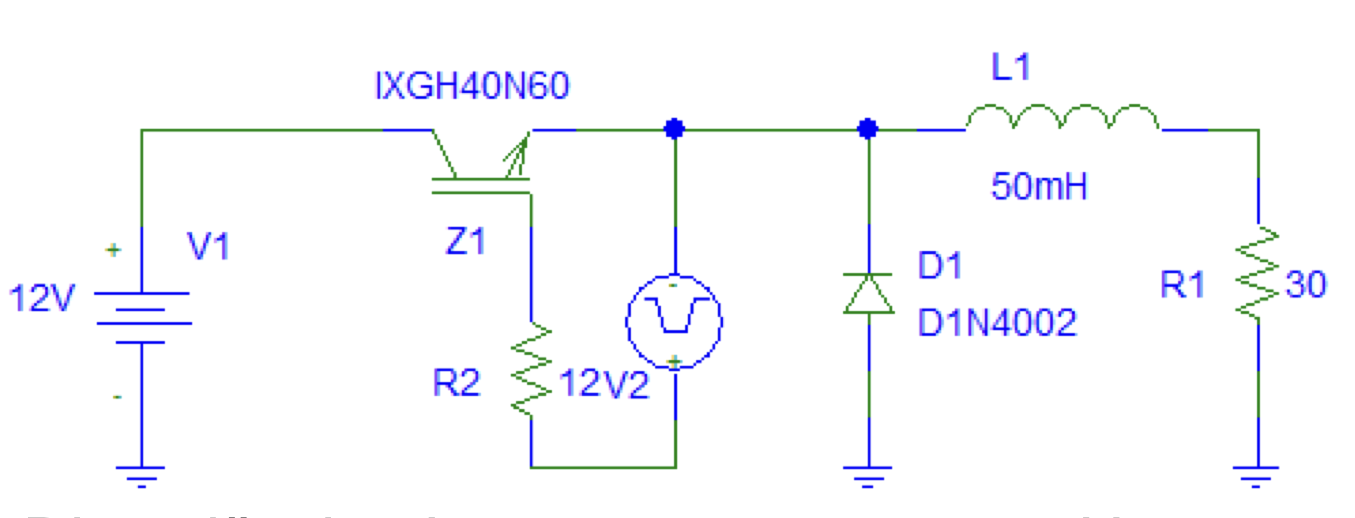
\includegraphics[width=0.85\linewidth]{images/Buckconverter.png}
\end{center}

Zeitverlauf Buck-Converter:
\begin{center}
    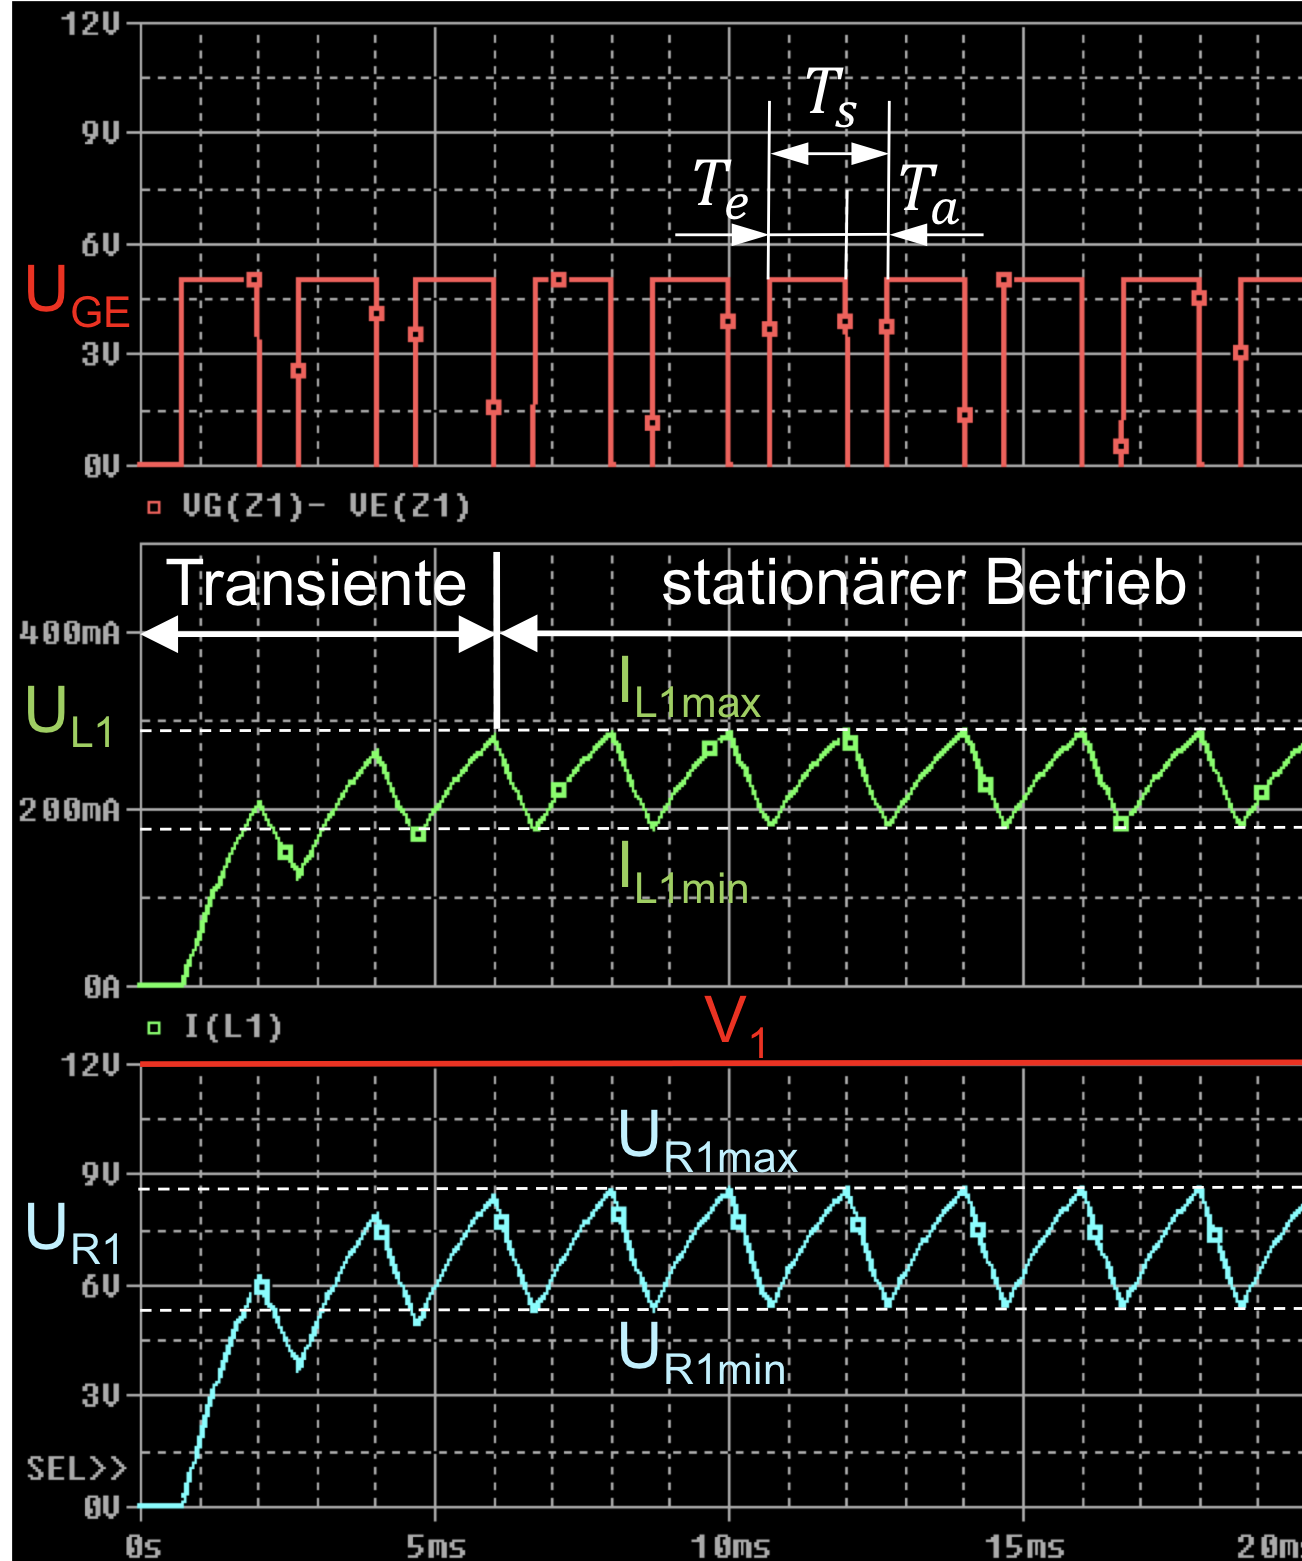
\includegraphics[width=0.85\linewidth]{images/Buckconverter_verlauf.png}
\end{center}

Ziel:
\[
u_2 < U_{DC}
\]

\paragraph{Voltsekunden-Bilanz}
\[
(U_{DC}-u_2)\, dT_s + (-u_2)(1-d)T_s = 0
\qquad\Rightarrow\qquad
\cbl{u_2 = d\,U_{DC}}
\]

\paragraph{EIN- und AUS-Gleichungen}

EIN-Phase:
\[
u_L = U_{DC} - u_2,
\qquad
i_C = i_L - i_o
\]

AUS-Phase:
\[
u_L = -u_2,
\qquad
i_C = i_L - i_o
\]

\paragraph{Strom- und Spannungsripple}

\[
\Delta i_L = \frac{(U_{DC}-u_2)}{L} \, d T_s
\]

\[
\Delta u_2 \approx \frac{\Delta i_L}{8 f_s C}
\]

Eigenschaften:
\begin{itemize}
    \item Ausgangsspannung kleiner als Eingang
    \item Kontinuierlicher Ausgangsstrom
\end{itemize}

% -------------------------------------------------
\subsection{Boost-Converter (Aufwärtssteller)}

\begin{center}
    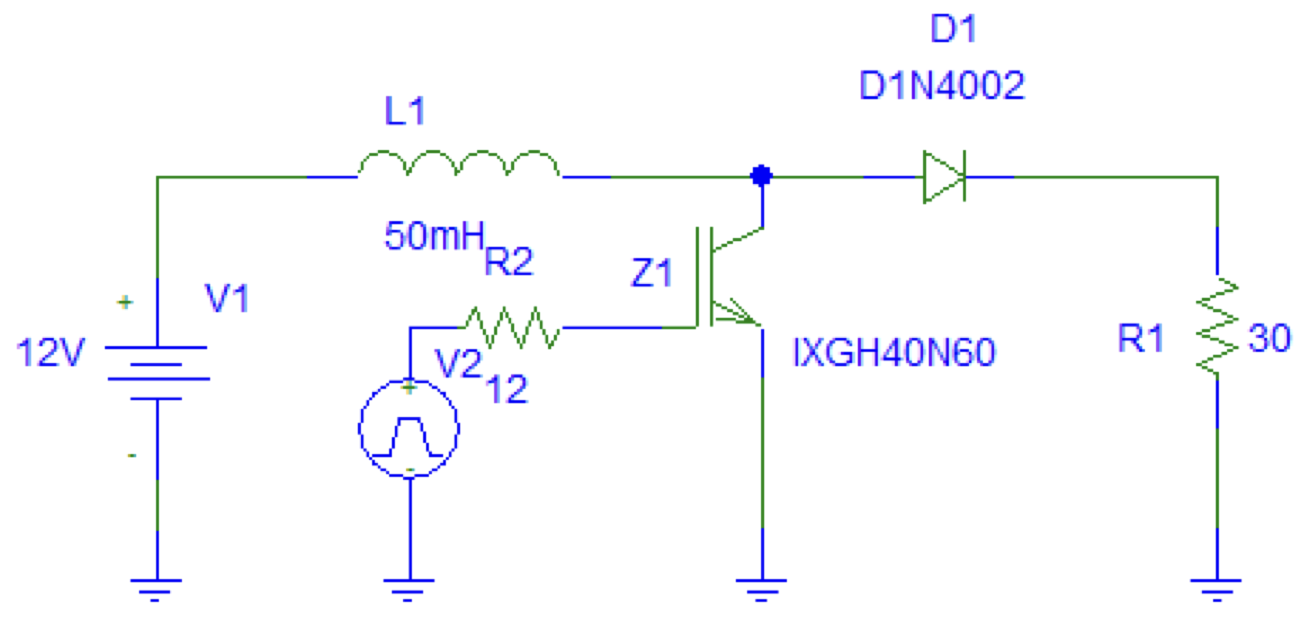
\includegraphics[width=0.85\linewidth]{images/Boostconv.png}
\end{center}

Zeitverlauf Boost-Converter:
\begin{center}
    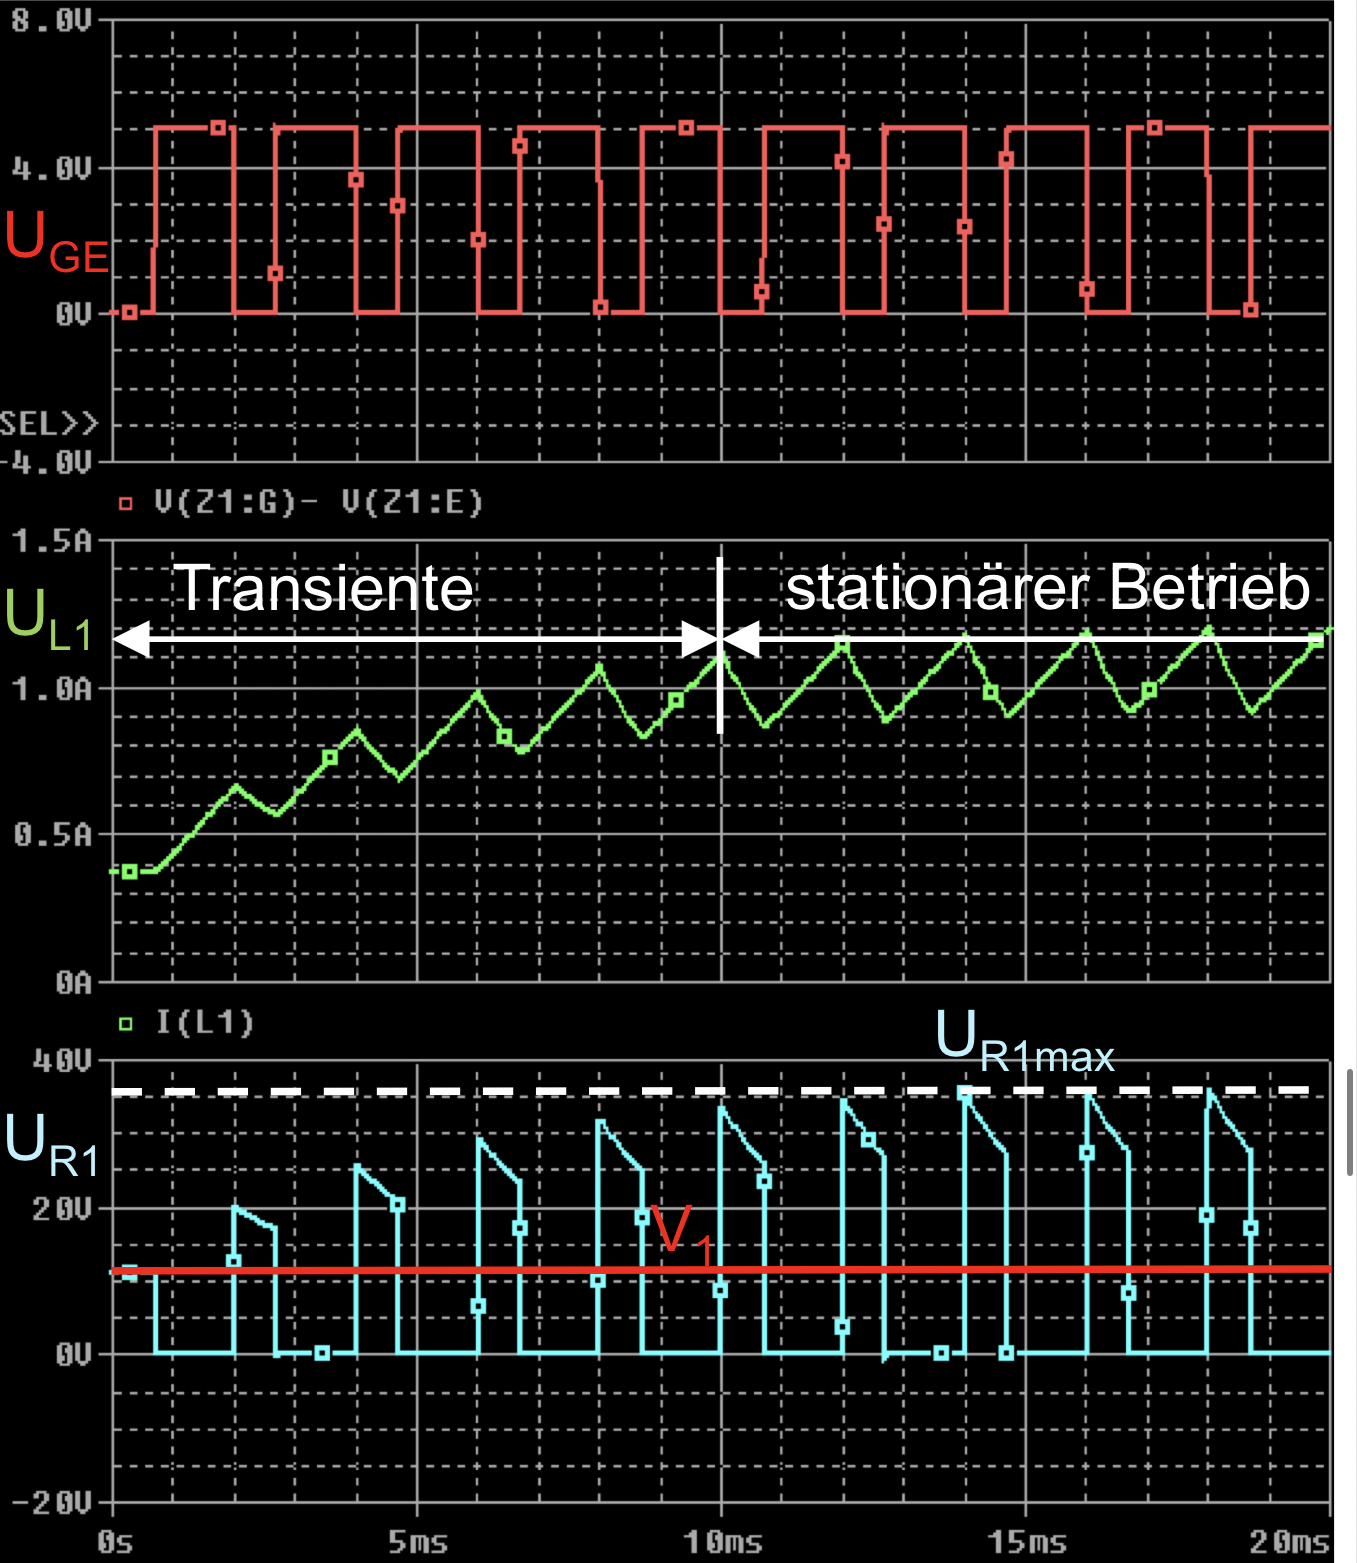
\includegraphics[width=0.85\linewidth]{images/Boostconv_verlauf.png}
\end{center}

Ziel:
\[
u_2 > U_{DC}
\]

\paragraph{Voltsekunden-Bilanz}
\[
U_{DC}\, dT_s + (U_{DC}-u_2)(1-d)T_s = 0
\qquad\Rightarrow\qquad
\cbl{u_2 = \frac{U_{DC}}{1-d}}
\]

\paragraph{EIN- und AUS-Gleichungen}

EIN-Phase (Diode sperrt):
\[
u_L = U_{DC},
\qquad
i_C = - i_o
\]

AUS-Phase (Diode leitet):
\[
u_L = U_{DC} - u_2,
\qquad
i_C = i_L - i_o
\]

\paragraph{Ripple-Näherungen}

\[
\Delta i_L = \frac{U_{DC}}{L} \, d T_s
\]

\[
\Delta u_2 \approx \frac{i_o}{C} (1-d) T_s
\]

Eigenschaften:
\begin{itemize}
    \item Ausgangsspannung grösser als Eingang
    \item Eingangsstrom gepulst
\end{itemize}

% -------------------------------------------------
\subsection{Buck-Boost-Converter}

\begin{center}
    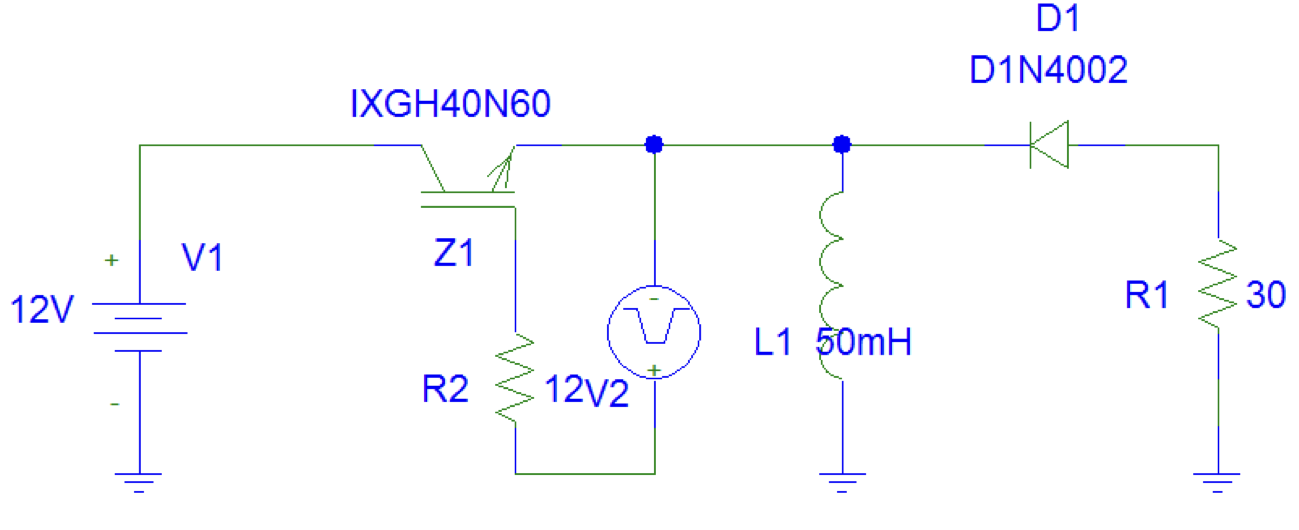
\includegraphics[width=0.85\linewidth]{images/Buckboostconv.png}
\end{center}

Zeitverlauf Buck-Boost-Converter:
\begin{center}
    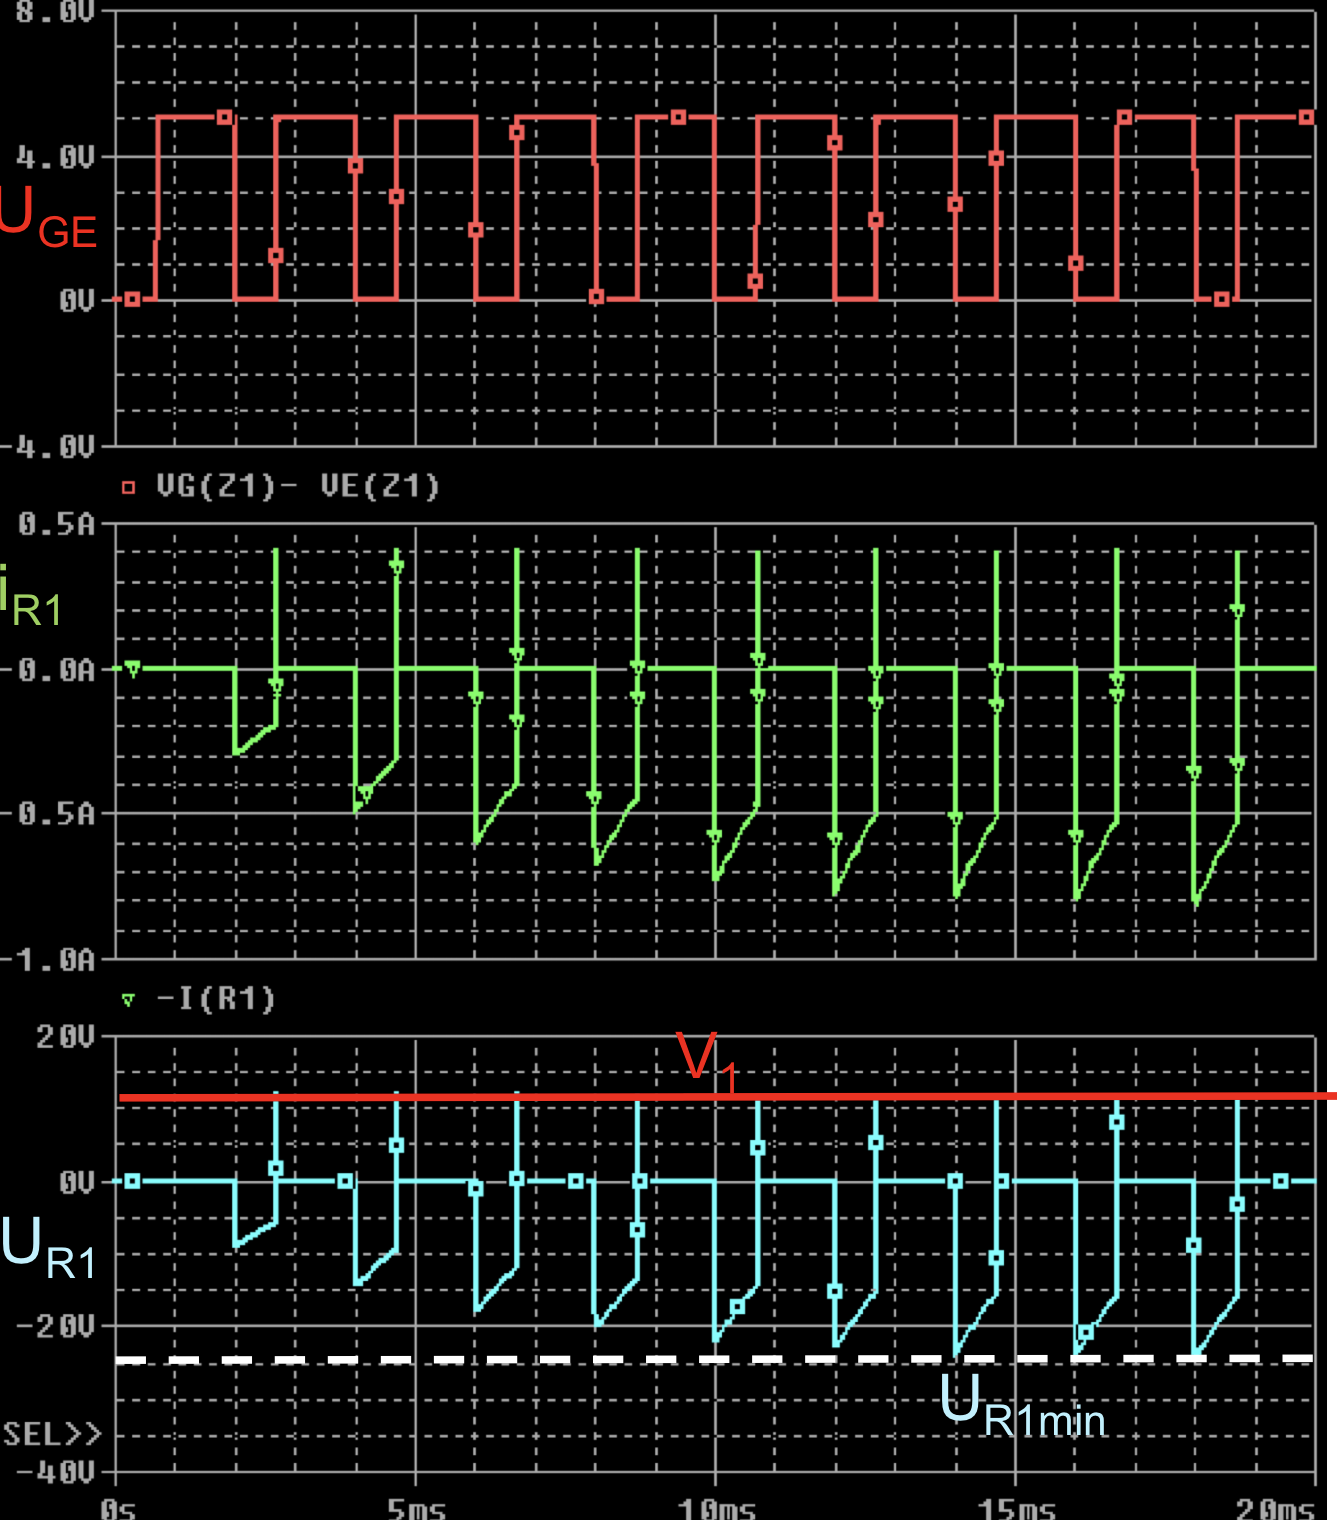
\includegraphics[width=0.85\linewidth]{images/Buckboostconv_verlauf.png}
\end{center}

Ziel:
\[
u_2 < 0 \quad \text{oder} \quad |u_2| > U_{DC}
\]

\paragraph{Voltsekunden-Bilanz}
\[
U_{DC}\, dT_s + (-u_2)(1-d)T_s = 0
\qquad\Rightarrow\qquad
\cbl{u_2 = -\frac{d}{1-d} U_{DC}}
\]

\paragraph{EIN- und AUS-Gleichungen}

EIN-Phase:
\[
u_L = U_{DC},
\qquad
i_C = - i_o
\]

AUS-Phase:
\[
u_L = -u_2,
\qquad
i_C = i_L - i_o
\]

\paragraph{Ripple-Näherungen}

\[
\Delta i_L = \frac{U_{DC}}{L} \, d T_s
\]

\[
\Delta u_2 \approx \frac{i_o}{C} (1-d) T_s
\]

Eigenschaften:
\begin{itemize}
    \item Polaritätsumkehr
    \item Spannung grösser oder kleiner als Eingang möglich
\end{itemize}

% -------------------------------------------------
\subsection{Vergleich der DC-DC-Wandler}

\begin{center}
\begin{tabular}{l|c|c|c}
 & Buck & Boost & Buck-Boost \\ \hline
$u_2/U_{DC}$ & $d$ & $\frac{1}{1-d}$ & $-\frac{d}{1-d}$ \\
Polarität & gleich & gleich & \cbl{invertiert} \\
$u_2<U_{DC}$ & \cbl{ja} & nein & ja \\
$u_2>U_{DC}$ & nein & \cbl{ja} & ja \\
\end{tabular}
\end{center}

% -------------------------------------------------
\subsection{Allgemeines Lösungsschema für Prüfungsaufgaben}

\begin{enumerate}
    \item Topologie identifizieren (Buck, Boost, Buck-Boost).
    \item Betriebsart prüfen: CCM oder DCM.
    \item EIN- und AUS-Gleichungen für $u_L$ und $i_C$ angeben.
    \item Voltsekunden-Bilanz $\overline{u_L}=0$ anwenden.
    \item Stromripple $\Delta i_L$ berechnen.
    \item Spannungsripple $\Delta u_2$ aus $C$ bestimmen.
    \item Falls Zeitbereich gefragt: Exponential- oder lineare Lösungen anwenden.
\end{enumerate}

\subsection{Abgrenzung zu klassischen Gleichstromstellern}

\begin{itemize}
    \item Klassischer Gleichstromsteller: direkte Pulsweitensteuerung der Last.
    \item DC-DC-Wandler: Energieübertragung über Induktivität mit Spannungsanpassung.
\end{itemize}

\crd{\textrightarrow\ Buck/Boost/Buck-Boost sind Gleichstromsteller mit Energiespeicher.}

        \section{Einführung in Gleichrichter und Grundsystematik}

Gleichrichter dienen der Umwandlung von Wechselspannung in Gleichspannung.
Sie bilden die Eingangsstufe nahezu aller leistungselektronischen Systeme,
insbesondere in Netzteilen, Umrichtern und elektrischen Antrieben.

Je nach Schaltungstopologie, Pulszahl und Steuerart ergeben sich sehr unterschiedliche
Eigenschaften hinsichtlich Mittelwert, Restwelligkeit, Netzrückwirkungen und Stellbarkeit.

\subsection{Systematik der Gleichrichterbezeichnungen}

Die Bezeichnungen der Gleichrichter folgen einer einheitlichen Nomenklatur,
die unmittelbar Auskunft über Aufbau und Funktion gibt:

\begin{itemize}
\item \textbf{M} = Mittelpunktschaltung,
\item \textbf{B} = Brückenschaltung,
\item \textbf{Zahl} = Pulszahl $p$ pro Netzperiode,
\item \textbf{U} = ungesteuert (Dioden),
\item \textbf{C} = gesteuert (Thyristoren).
\end{itemize}

Beispiele:
\begin{itemize}
\item M1U: Einpuls, Mittelpunkt, ungesteuert,
\item B2U: Zweipuls, Brücke, ungesteuert,
\item B6C: Sechspuls, Brücke, gesteuert.
\end{itemize}

Die Pulszahl bestimmt die Frequenz der Gleichspannungswelligkeit
und damit die Qualität der erzeugten Gleichspannung.

\crd{\textrightarrow\ M/B beschreibt die Topologie, die Zahl die Pulszahl, U/C die Steuerart.}

\subsection{Grundklassifikation der Gleichrichter}

Man unterscheidet grundsätzlich zwei Hauptklassen:

\begin{itemize}
\item \textbf{Ungesteuerte Gleichrichter (U)}:  
Dioden, keine Stellmöglichkeit der Ausgangsspannung.

\item \textbf{Gesteuerte Gleichrichter (C)}:  
Thyristoren, Stellgrösse ist der Zündwinkel $\alpha$.
\end{itemize}

Bei gesteuerten Gleichrichtern ist der Mittelwert der Gleichspannung
proportional zu $\cos\alpha$.
Für $\alpha > 90^\circ$ ist Rückspeisebetrieb möglich.

\subsection{Einfluss von Induktivität und Kapazität auf den Betrieb}

In realen Anwendungen werden Induktivität $L$ und Kapazität $C$ eingesetzt,
um das Verhalten des Gleichrichters gezielt zu beeinflussen.
Sie bestimmen wesentlich die Stromform, die Spannungswelligkeit
sowie die Netzrückwirkungen.

Man unterscheidet drei Grundfälle:

\begin{itemize}
\item \textbf{C-Glättung (kapazitive Last)},
\item \textbf{L-Glättung (induktive Last)},
\item \textbf{LC-Glättung (Filter)}.
\end{itemize}

Der gewählte Lasttyp bestimmt insbesondere:

\begin{itemize}
\item die Stromform $i_d(t)$ im Gleichrichter,
\item die Restwelligkeit der Gleichspannung $\Delta u_d$,
\item die Netzstromharmonischen,
\item den Leistungsfaktor $\lambda$,
\item die thermische Belastung der Halbleiter.
\end{itemize}

\subsubsection*{C-Glättung (kapazitive Last)}

Der Kondensator lädt sich in jeder Leitphase auf den momentanen Scheitelwert
der Gleichspannung auf und entlädt sich zwischen den Leitphasen über die Last.

Näherung für den Spannungsrippel:
\[
\cbl{\Delta u_d \approx \frac{I_d}{f_r \, C}}
\]
mit:
\begin{itemize}
\item $I_d$: mittlerer Gleichstrom,
\item $f_r = p f$: Ripple-Frequenz der Gleichspannung,
\item $p$: Pulszahl des Gleichrichters,
\item $f$: Netzfrequenz,
\item $C$: Kapazität des Kondensators.
\end{itemize}

Mittelwert der Gleichspannung:
\[
\cbl{u_d \approx \hat U_d - \frac{\Delta u_d}{2}}
\]
mit:
\begin{itemize}
\item $\hat U_d$: Scheitelwert der gleichgerichteten Spannung.
\end{itemize}

Typische Konsequenzen:
\begin{itemize}
\item Sehr kurze Leitwinkel $\Rightarrow$ hohe Spitzenströme:
\[
\cbl{i_{D,\max} \gg I_d}
\]
\item Starke Verzerrung des Netzstroms.
\item Schlechter Leistungsfaktor:
\[
\cbl{\lambda = \frac{P}{U_{\mathrm{RMS}} I_{\mathrm{RMS}}} \ll 1}
\]
\end{itemize}

\subsubsection*{L-Glättung (induktive Last)}

Die Induktivität erzwingt eine nahezu konstante Stromform.
Im stationären Betrieb gilt für die mittlere Induktorspannung:

\[
\cbl{\overline{u_L} = \frac{1}{T}\int_0^T u_L(t)\, dt = 0}
\]

Mit:
\[
u_L(t) = L \frac{di_d(t)}{dt}
\]

Daraus folgt für den Mittelwert der Gleichspannung:
\[
\cbl{u_d = \overline{u_{\mathrm{gr}}(t)}}
\]
mit:
\begin{itemize}
\item $u_{\mathrm{gr}}(t)$: momentane gleichgerichtete Spannung.
\end{itemize}

Stromwelligkeit:
\[
\cbl{\Delta i_d \approx \frac{\Delta u_d}{\omega L}}
\]

Typische Konsequenzen:
\begin{itemize}
\item Nahezu konstanter Gleichstrom:
\[
\cbl{i_d(t) \approx I_d = \text{konstant}}
\]
\item Rechteckförmige Netzströme bei Mehrpuls-Gleichrichtern.
\item Geringere Oberschwingungen als bei C-Glättung.
\item Besserer Leistungsfaktor:
\[
\cbl{\lambda \uparrow}
\]
\end{itemize}

\subsubsection*{LC-Glättung (Tiefpassfilter)}

Die Kombination aus Serieninduktivität und Parallel-Kondensator
bildet ein Tiefpassfilter für die Gleichspannung.

Grenzfrequenz des Filters:
\[
\cbl{\omega_0 = \frac{1}{\sqrt{LC}}}
\qquad
f_0 = \frac{1}{2\pi\sqrt{LC}}
\]

Übertragungsverhalten:
\[
|H(j\omega)| \approx
\begin{cases}
1, & \omega \ll \omega_0, \\
\downarrow, & \omega \gg \omega_0.
\end{cases}
\]

Dämpfung der Ripple-Komponente:
\[
\cbl{\Delta u_d \propto |H(j\omega_r)|}
\]
mit:
\begin{itemize}
\item $\omega_r = 2\pi f_r$: Ripple-Kreisfrequenz.
\end{itemize}

Typische Konsequenzen:
\begin{itemize}
\item Sehr geringe Restwelligkeit der Gleichspannung.
\item Gute Strom- und Spannungsqualität.
\item Höherer Bauteilaufwand.
\end{itemize}


\subsection{Ziel der folgenden Kapitel}

In den folgenden Kapiteln werden systematisch behandelt:

\begin{itemize}
\item Einpuls-Gleichrichter (M1U, M1C),
\item Zweipuls-Gleichrichter (B2U, B2C),
\item Dreiphasige Gleichrichter (B6U, B6C),
\item Einfluss von Last, Steuerung und Netzinduktivität,
\item Netzrückwirkungen und Harmonische.
\end{itemize}

Ziel ist eine einheitliche Beschreibung aller Gleichrichter
auf Basis von:

\begin{itemize}
\item Pulszahl $p$,
\item Steuerart (U/C),
\item Leitwinkel $\alpha$, $\beta$,
\item Mittelwert- und Verlustgleichungen.
\end{itemize}


\subsection{M1U: Ungesteuerter Einpuls-Gleichrichter}

% --- bestehende Grafik: Schaltung ---
\begin{center}
    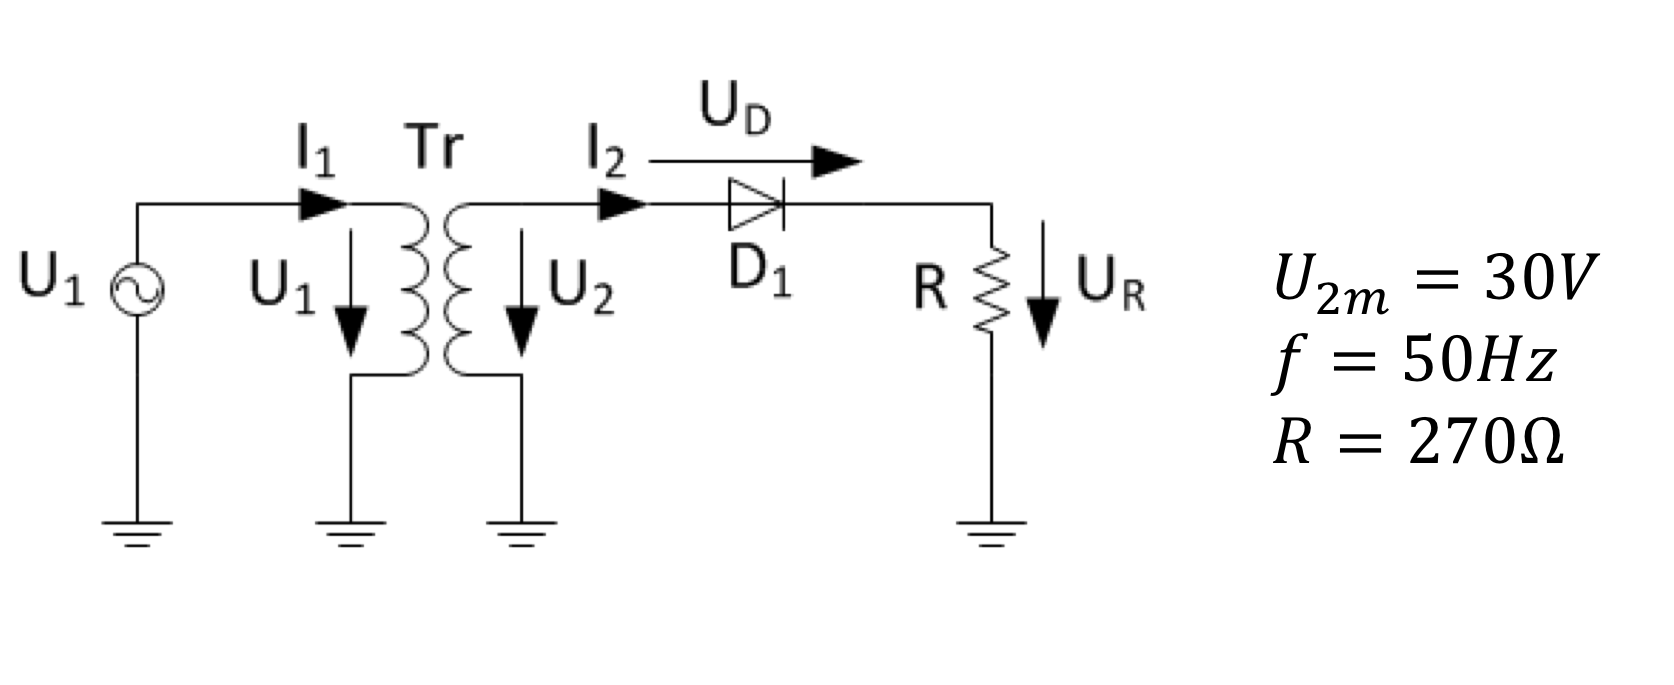
\includegraphics[width=0.85\linewidth]{images/M1U.png}
\end{center}

Der ungesteuerte Einpuls-Gleichrichter besteht aus einer Diode und einer einphasigen Wechselspannungsquelle.
Er arbeitet ohne Stellmöglichkeit und liefert eine pulsierende Gleichspannung mit der Pulszahl $p=1$.

Eingangsspannung:
\[
u_s(t) = \hat U \sin(\omega t)
\]
mit:
\begin{itemize}
\item $\hat U$: Scheitelwert der Eingangsspannung,
\item $\omega = 2\pi f$: Kreisfrequenz,
\item $f$: Netzfrequenz.
\end{itemize}

Momentane Ausgangsspannung:
\[
u_d(t) =
\begin{cases}
\hat U \sin(\omega t), & \sin(\omega t) \ge 0, \\
0, & \sin(\omega t) < 0.
\end{cases}
\]

Mittelwert der Gleichspannung:
\[
\cbl{\overline{u_d} = \frac{1}{2\pi}\int_0^{\pi} \hat U \sin\gamma \, d\gamma
= \frac{\hat U}{\pi}}
\]
mit:
\begin{itemize}
\item $\gamma = \omega t$: elektrischer Winkel.
\end{itemize}

Effektivwert der Ausgangsspannung:
\[
\cbl{U_{d,\mathrm{RMS}} = \sqrt{\frac{1}{2\pi}\int_0^{\pi} \hat U^2 \sin^2\gamma \, d\gamma}
= \frac{\hat U}{2}}
\]

Mittelwert des Gleichstroms bei ohmscher Last $R$:
\[
\cbl{I_d = \frac{\overline{u_d}}{R} = \frac{\hat U}{\pi R}}
\]

Effektivwert des Stroms:
\[
\cbl{I_{d,\mathrm{RMS}} = \frac{U_{d,\mathrm{RMS}}}{R} = \frac{\hat U}{2R}}
\]

Leistungsaufnahme an ohmscher Last:
\[
\cbl{P = R I_{d,\mathrm{RMS}}^2 = \frac{\hat U^2}{4R}}
\]

Eigenschaften:
\begin{itemize}
\item Keine Stellmöglichkeit der Ausgangsspannung.
\item Sehr hohe Restwelligkeit der Gleichspannung.
\item Geringe Gleichspannungsqualität.
\item Einfachste Gleichrichterschaltung.
\end{itemize}

% --- bestehende Grafik: Spannungsverlauf ---
\begin{center}
    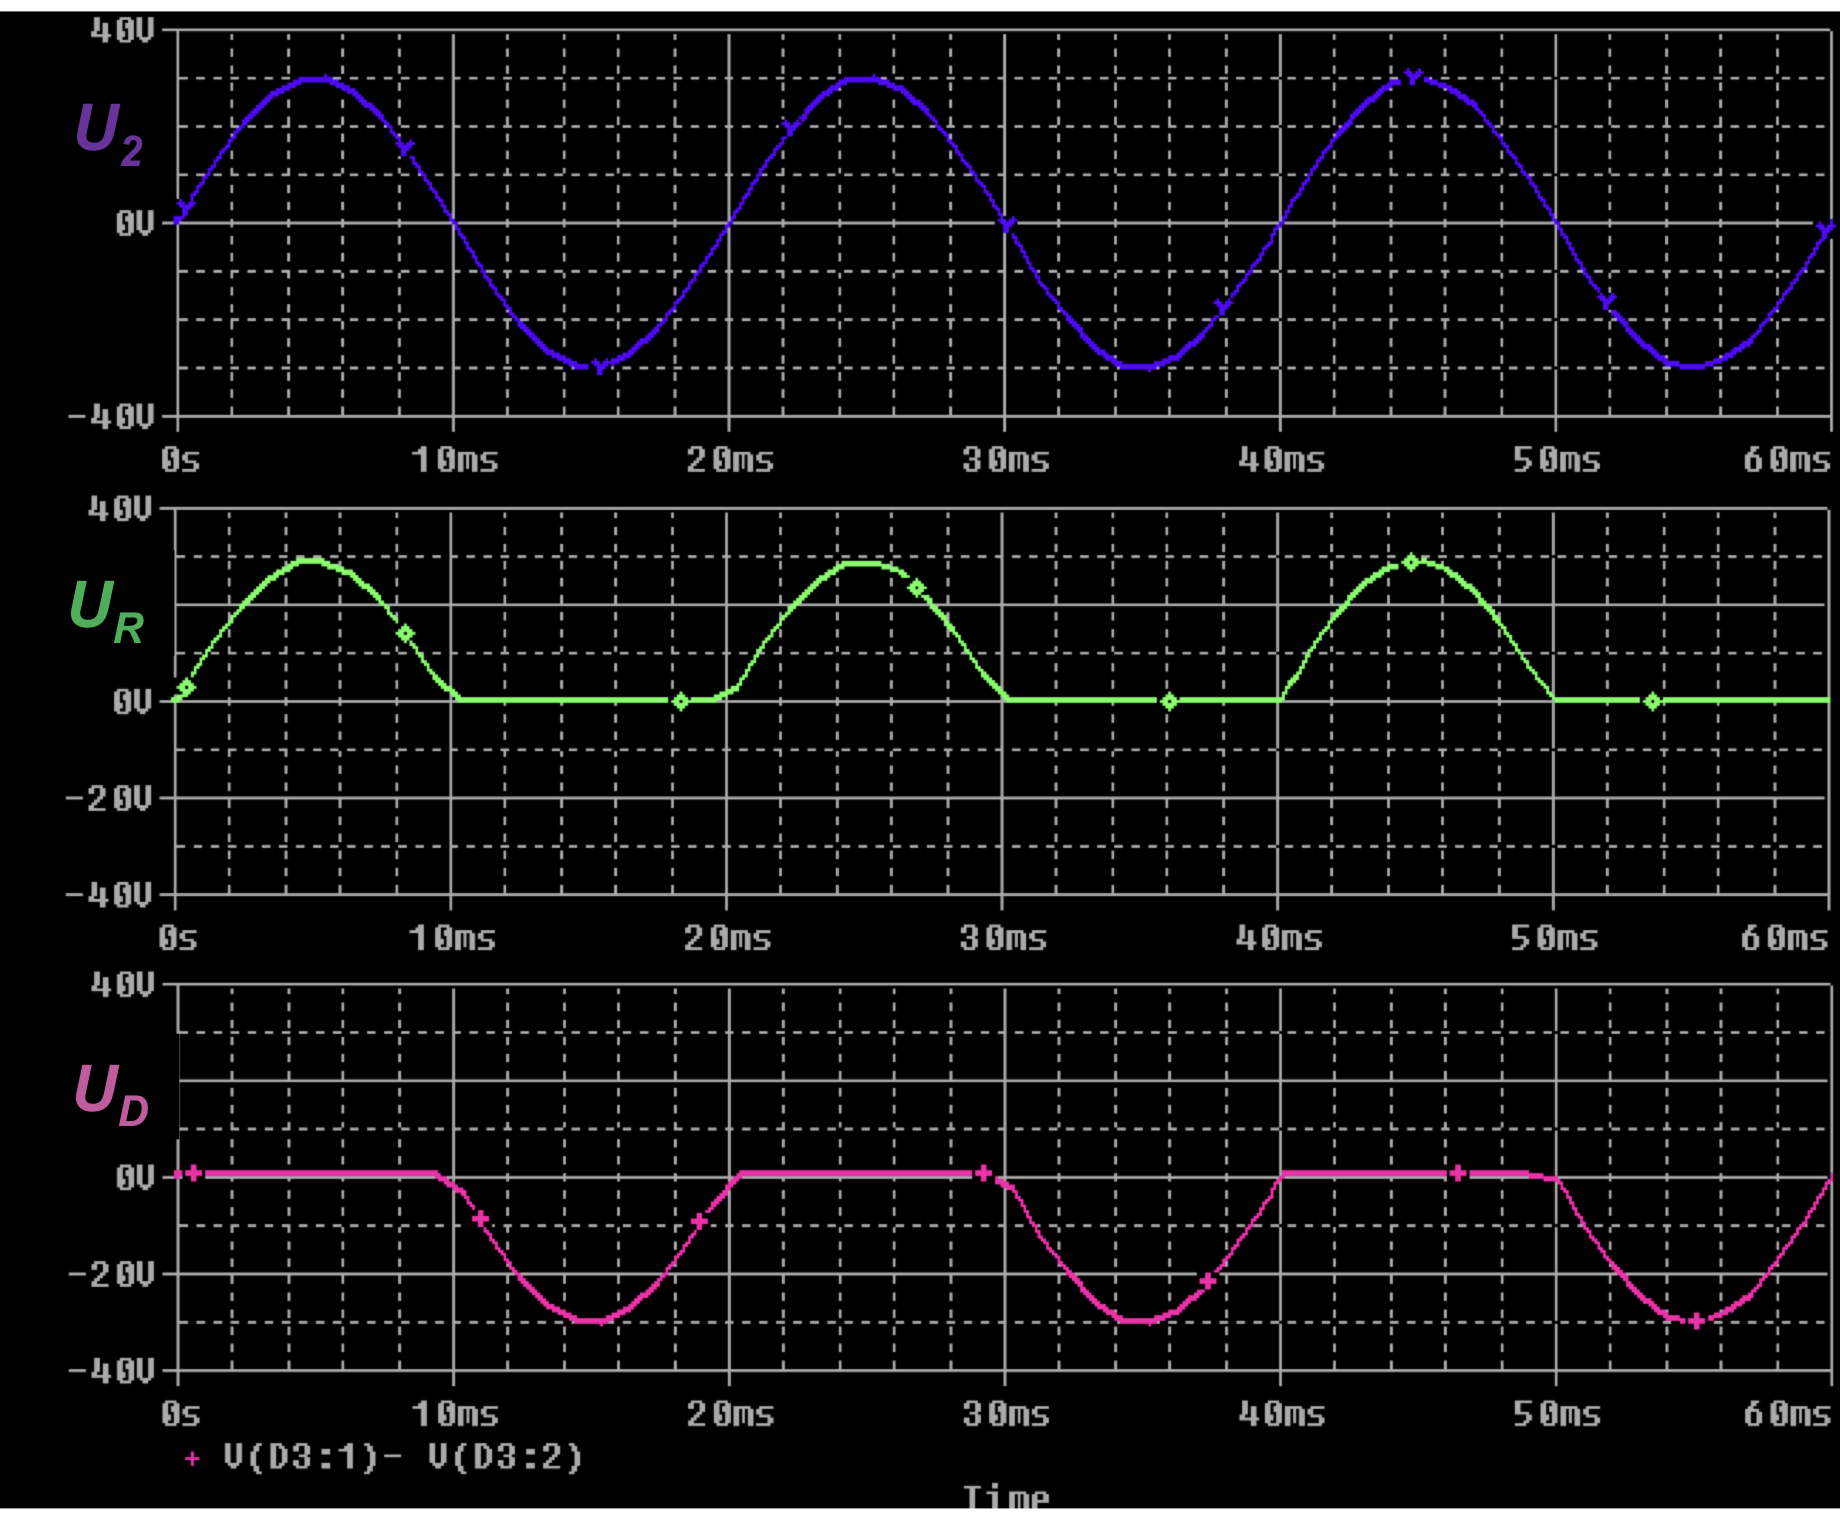
\includegraphics[width=0.85\linewidth]{images/M1U_verlauf.png}
\end{center}

\subsection{M1C: Gesteuerter Einpuls-Gleichrichter}

% --- bestehende Grafik: Schaltung ---
\begin{center}
    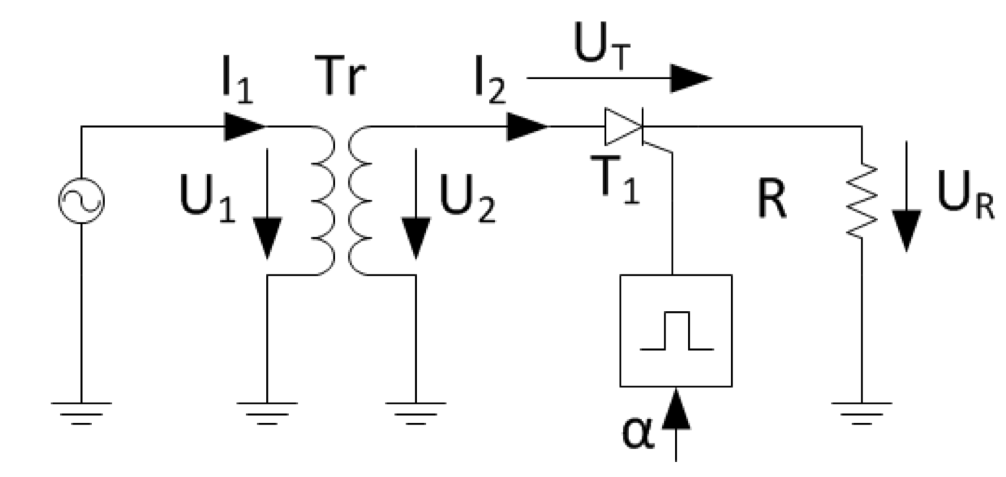
\includegraphics[width=0.85\linewidth]{images/M1C.png}
\end{center}

Der gesteuerte Einpuls-Gleichrichter ersetzt die Diode durch einen Thyristor.
Der Leitbeginn wird durch den Zündwinkel $\alpha$ gesteuert.

Eingangsspannung:
\[
u_s(t) = \hat U \sin(\omega t)
\]
mit:
\begin{itemize}
\item $\hat U$: Scheitelwert der Eingangsspannung,
\item $\omega = 2\pi f$: Kreisfrequenz,
\item $f$: Netzfrequenz.
\end{itemize}

Leitbedingung:
\[
\boxed{\omega t \ge \alpha}
\]

Momentane Ausgangsspannung:
\[
u_d(t) =
\begin{cases}
\hat U \sin(\omega t), & \omega t \ge \alpha, \\
0, & \omega t < \alpha.
\end{cases}
\]

Mittelwert der Gleichspannung:
\[
\cbl{\overline{u_d}
= \frac{1}{2\pi}\int_{\alpha}^{\pi} \hat U \sin\gamma \, d\gamma
= \frac{\hat U}{2\pi}(1+\cos\alpha)}
\]

Stellbereich:
\[
0 \le \alpha \le \pi
\]

Grenzfälle:
\[
\alpha = 0 \Rightarrow \overline{u_d} = \frac{\hat U}{\pi}
\]
\[
\alpha = \pi \Rightarrow \overline{u_d} = 0
\]

Mittelwert des Stroms bei ohmscher Last $R$:
\[
\cbl{I_d = \frac{\overline{u_d}}{R}
= \frac{\hat U}{2\pi R}(1+\cos\alpha)}
\]

Effektivwert der Ausgangsspannung:
\[
\cbl{U_{d,\mathrm{RMS}}
= \sqrt{\frac{1}{2\pi}\int_{\alpha}^{\pi} \hat U^2 \sin^2\gamma \, d\gamma}}
\]

Leistungsaufnahme an ohmscher Last:
\[
\cbl{P = R I_{d,\mathrm{RMS}}^2}
\]

Eigenschaften:
\begin{itemize}
\item Stellbare Gleichspannung über den Zündwinkel $\alpha$.
\item Bei $\alpha = 0$: Verhalten wie M1U.
\item Bei $\alpha > 90^\circ$: negativer Mittelwert möglich (in geeigneter Schaltung Rückspeisung).
\item Einfachster gesteuerter Gleichrichter.
\end{itemize}

% --- bestehende Grafik: Spannungsverlauf ---
\begin{center}
    \includegraphics[width=0.85\linewidth]{images/M1C_verlauf.png}
\end{center}

\subsection{B2U: Ungesteuerter Zweipuls-Gleichrichter}

% --- bestehende Grafik: Schaltung ---
\begin{center}
    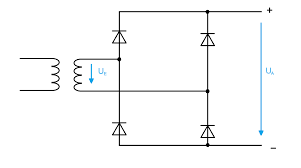
\includegraphics[width=0.85\linewidth]{images/B2U.png}
\end{center}

Der ungesteuerte Zweipuls-Gleichrichter ist eine vollwellige Brückenschaltung mit vier Dioden.
Er nutzt beide Halbwellen der Eingangsspannung und besitzt die Pulszahl $p=2$.

Eingangsspannung:
\[
u_s(t) = \hat U \sin(\omega t)
\]
mit:
\begin{itemize}
\item $\hat U$: Scheitelwert der Eingangsspannung,
\item $\omega = 2\pi f$: Kreisfrequenz,
\item $f$: Netzfrequenz.
\end{itemize}

Momentane Ausgangsspannung:
\[
u_d(t) = |u_s(t)| = |\hat U \sin(\omega t)|
\]

Mittelwert der Gleichspannung:
\[
\cbl{\overline{u_d}
= \frac{1}{\pi}\int_{0}^{\pi} \hat U \sin\gamma \, d\gamma
= \frac{2\hat U}{\pi}}
\]
mit:
\begin{itemize}
\item $\gamma = \omega t$: elektrischer Winkel.
\end{itemize}

Effektivwert der Ausgangsspannung:
\[
\cbl{U_{d,\mathrm{RMS}}
= \sqrt{\frac{1}{\pi}\int_{0}^{\pi} \hat U^2 \sin^2\gamma \, d\gamma}
= \frac{\hat U}{\sqrt{2}}}
\]

Mittelwert des Gleichstroms bei ohmscher Last $R$:
\[
\cbl{I_d = \frac{\overline{u_d}}{R} = \frac{2\hat U}{\pi R}}
\]

Effektivwert des Stroms:
\[
\cbl{I_{d,\mathrm{RMS}} = \frac{U_{d,\mathrm{RMS}}}{R}
= \frac{\hat U}{\sqrt{2}R}}
\]

Leistungsaufnahme an ohmscher Last:
\[
\cbl{P = R I_{d,\mathrm{RMS}}^2 = \frac{\hat U^2}{2R}}
\]

Restwelligkeit (Ripple-Faktor):
\[
\cbl{r = \frac{\sqrt{U_{d,\mathrm{RMS}}^2 - \overline{u_d}^2}}{\overline{u_d}}}
\]

Eigenschaften:
\begin{itemize}
\item Keine Stellmöglichkeit der Ausgangsspannung.
\item Deutlich geringere Welligkeit als beim M1U.
\item Doppelte Pulsfrequenz der Gleichspannung ($2f$).
\item Standard-Gleichrichter für einfache Anwendungen.
\end{itemize}

% --- bestehende Grafik: Spannungsverlauf ---
\begin{center}
    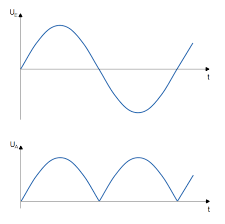
\includegraphics[width=0.85\linewidth]{images/B2U_verlauf.png}
\end{center}
\subsection{B2C: Gesteuerter Zweipuls-Gleichrichter}

% --- bestehende Grafik: Schaltung ---
\begin{center}
    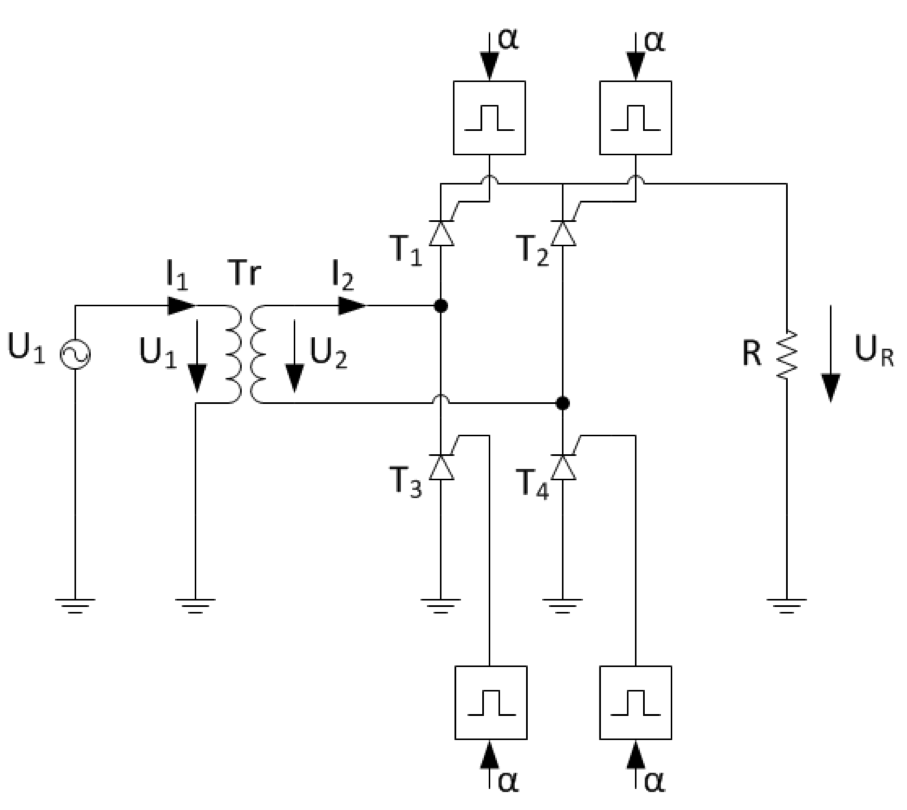
\includegraphics[width=0.85\linewidth]{images/B1C.png}
\end{center}

Der gesteuerte Zweipuls-Gleichrichter ersetzt die Dioden durch Thyristoren.
Der Leitbeginn wird über den Zündwinkel $\alpha$ gesteuert.

Eingangsspannung:
\[
u_s(t) = \hat U \sin(\omega t)
\]
mit:
\begin{itemize}
\item $\hat U$: Scheitelwert der Eingangsspannung,
\item $\omega = 2\pi f$: Kreisfrequenz,
\item $f$: Netzfrequenz.
\end{itemize}

Leitbedingung:
\[
\boxed{\omega t \ge \alpha}
\]

Momentane Ausgangsspannung:
\[
u_d(t) =
\begin{cases}
\hat U \sin(\omega t), & \omega t \ge \alpha, \\
0, & \omega t < \alpha.
\end{cases}
\]

Mittelwert der Gleichspannung:
\[
\cbl{\overline{u_d}
= \frac{1}{\pi}\int_{\alpha}^{\pi} \hat U \sin\gamma \, d\gamma
= \frac{2\hat U}{\pi}\cos\alpha}
\]

Stellbereich:
\[
0 \le \alpha \le \pi
\]

Grenzfälle:
\[
\alpha = 0 \Rightarrow \overline{u_d} = \frac{2\hat U}{\pi}
\]
\[
\alpha = \frac{\pi}{2} \Rightarrow \overline{u_d} = 0
\]
\[
\alpha > \frac{\pi}{2} \Rightarrow \overline{u_d} < 0 \quad \text{(Rückspeisebetrieb möglich)}
\]

Mittelwert des Stroms bei ohmscher Last $R$:
\[
\cbl{I_d = \frac{\overline{u_d}}{R}
= \frac{2\hat U}{\pi R}\cos\alpha}
\]

Effektivwert der Ausgangsspannung:
\[
\cbl{U_{d,\mathrm{RMS}}
= \sqrt{\frac{1}{\pi}\int_{\alpha}^{\pi} \hat U^2 \sin^2\gamma \, d\gamma}}
\]

Leistungsaufnahme an ohmscher Last:
\[
\cbl{P = R I_{d,\mathrm{RMS}}^2}
\]

Leistungsfaktor bei ohmscher Last:
\[
\cbl{\lambda = \frac{P}{U_{\mathrm{RMS}} I_{\mathrm{RMS}}}}
\]

Eigenschaften:
\begin{itemize}
\item Stellbare Gleichspannung über den Zündwinkel $\alpha$.
\item Mittelwert proportional zu $\cos\alpha$.
\item Rückspeisebetrieb für $\alpha > 90^\circ$.
\item Phasenanschnittsteuerung.
\end{itemize}

% --- bestehende Grafik: Zündwinkeldiagramm ---
\begin{center}
    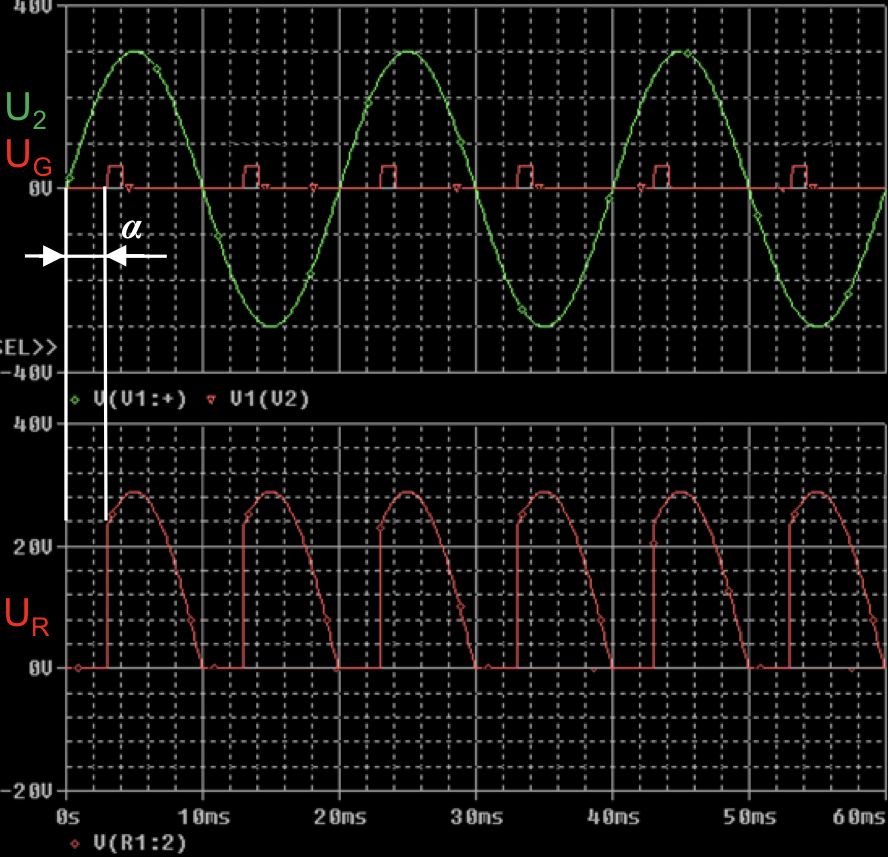
\includegraphics[width=0.85\linewidth]{images/B1C_Verlauf.png}
\end{center}

\subsection{B6U: Ungesteuerter Dreiphasen-Brückengleichrichter}

% --- bestehende Grafik: Schaltung ---
\begin{center}
    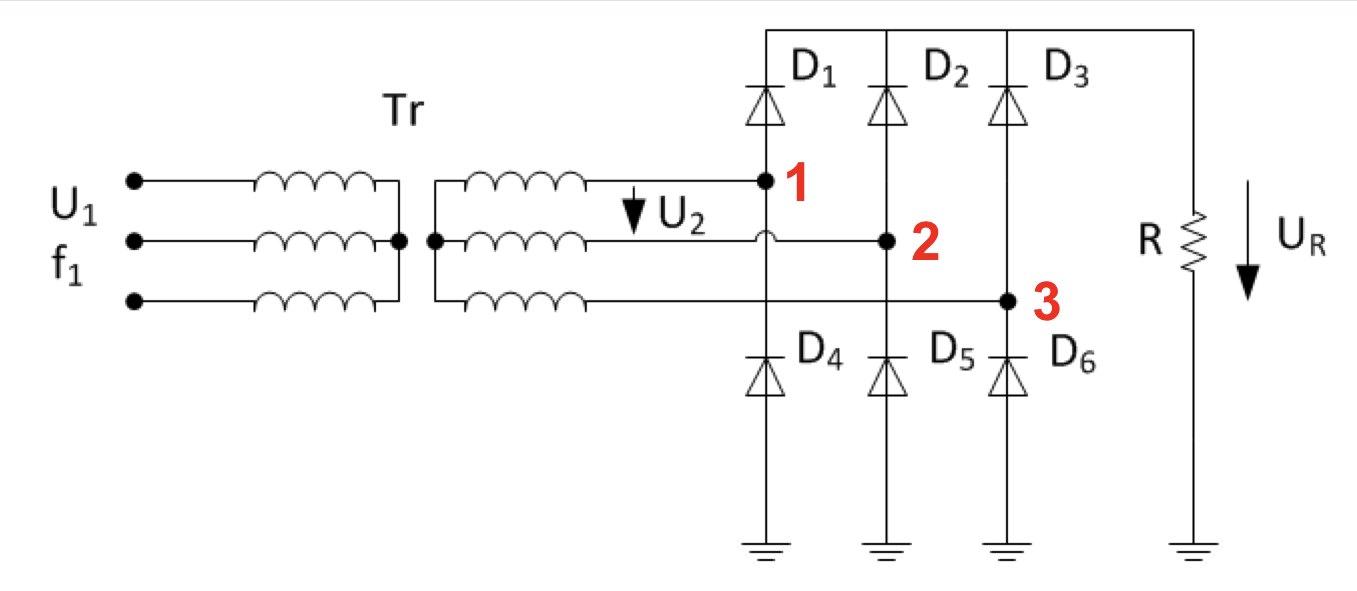
\includegraphics[width=0.65\linewidth]{images/B6U.png}
\end{center}

Der ungesteuerte Dreiphasen-Brückengleichrichter besteht aus sechs Dioden
und nutzt jeweils die beiden momentanen Leiterspannungen mit größtem Betrag.
Die Pulszahl beträgt $p=6$.

Eingangsspannungen:
\[
u_{ab}(t),\; u_{bc}(t),\; u_{ca}(t)
\]
mit:
\begin{itemize}
\item $U_{LL}$: Effektivwert der Leiterspannung,
\item $\hat U_{LL} = \sqrt{2} U_{LL}$: Scheitelwert der Leiterspannung,
\item $\omega = 2\pi f$: Kreisfrequenz,
\item $f$: Netzfrequenz.
\end{itemize}

Momentane Ausgangsspannung:
\[
u_d(t) = \max \{ u_{ab}(t),\, u_{bc}(t),\, u_{ca}(t),\, 0 \}
\]

Mittelwert der Gleichspannung:
\[
\cbl{\overline{u_d}
= \frac{3\sqrt{2}}{\pi} U_{LL}}
\]

Effektivwert der Gleichspannung (ideal, ohne Überlappung):
\[
\cbl{U_{d,\mathrm{RMS}}
= \sqrt{\frac{1}{2\pi}\int_0^{2\pi} u_d^2(\gamma)\, d\gamma}}
\]

Mittelwert des Gleichstroms bei ohmscher Last $R$:
\[
\cbl{I_d = \frac{\overline{u_d}}{R}
= \frac{3\sqrt{2}}{\pi}\frac{U_{LL}}{R}}
\]

Effektivwert des Gleichstroms:
\[
\cbl{I_{d,\mathrm{RMS}} = \frac{U_{d,\mathrm{RMS}}}{R}}
\]

Leistungsaufnahme an ohmscher Last:
\[
\cbl{P = R I_{d,\mathrm{RMS}}^2}
\]

Ripple-Frequenz der Gleichspannung:
\[
\cbl{f_r = p f = 6 f}
\]

Ripple-Faktor:
\[
\cbl{r = \frac{\sqrt{U_{d,\mathrm{RMS}}^2 - \overline{u_d}^2}}{\overline{u_d}}}
\]

Eigenschaften:
\begin{itemize}
\item Sehr geringe Restwelligkeit der Gleichspannung.
\item Hohe Gleichspannungsqualität.
\item Sehr gute Ausnutzung der Netzspannung.
\item Standard-Gleichrichter in Industrieanwendungen.
\end{itemize}

% --- bestehende Grafik: Spannungsverlauf ---
\begin{center}
    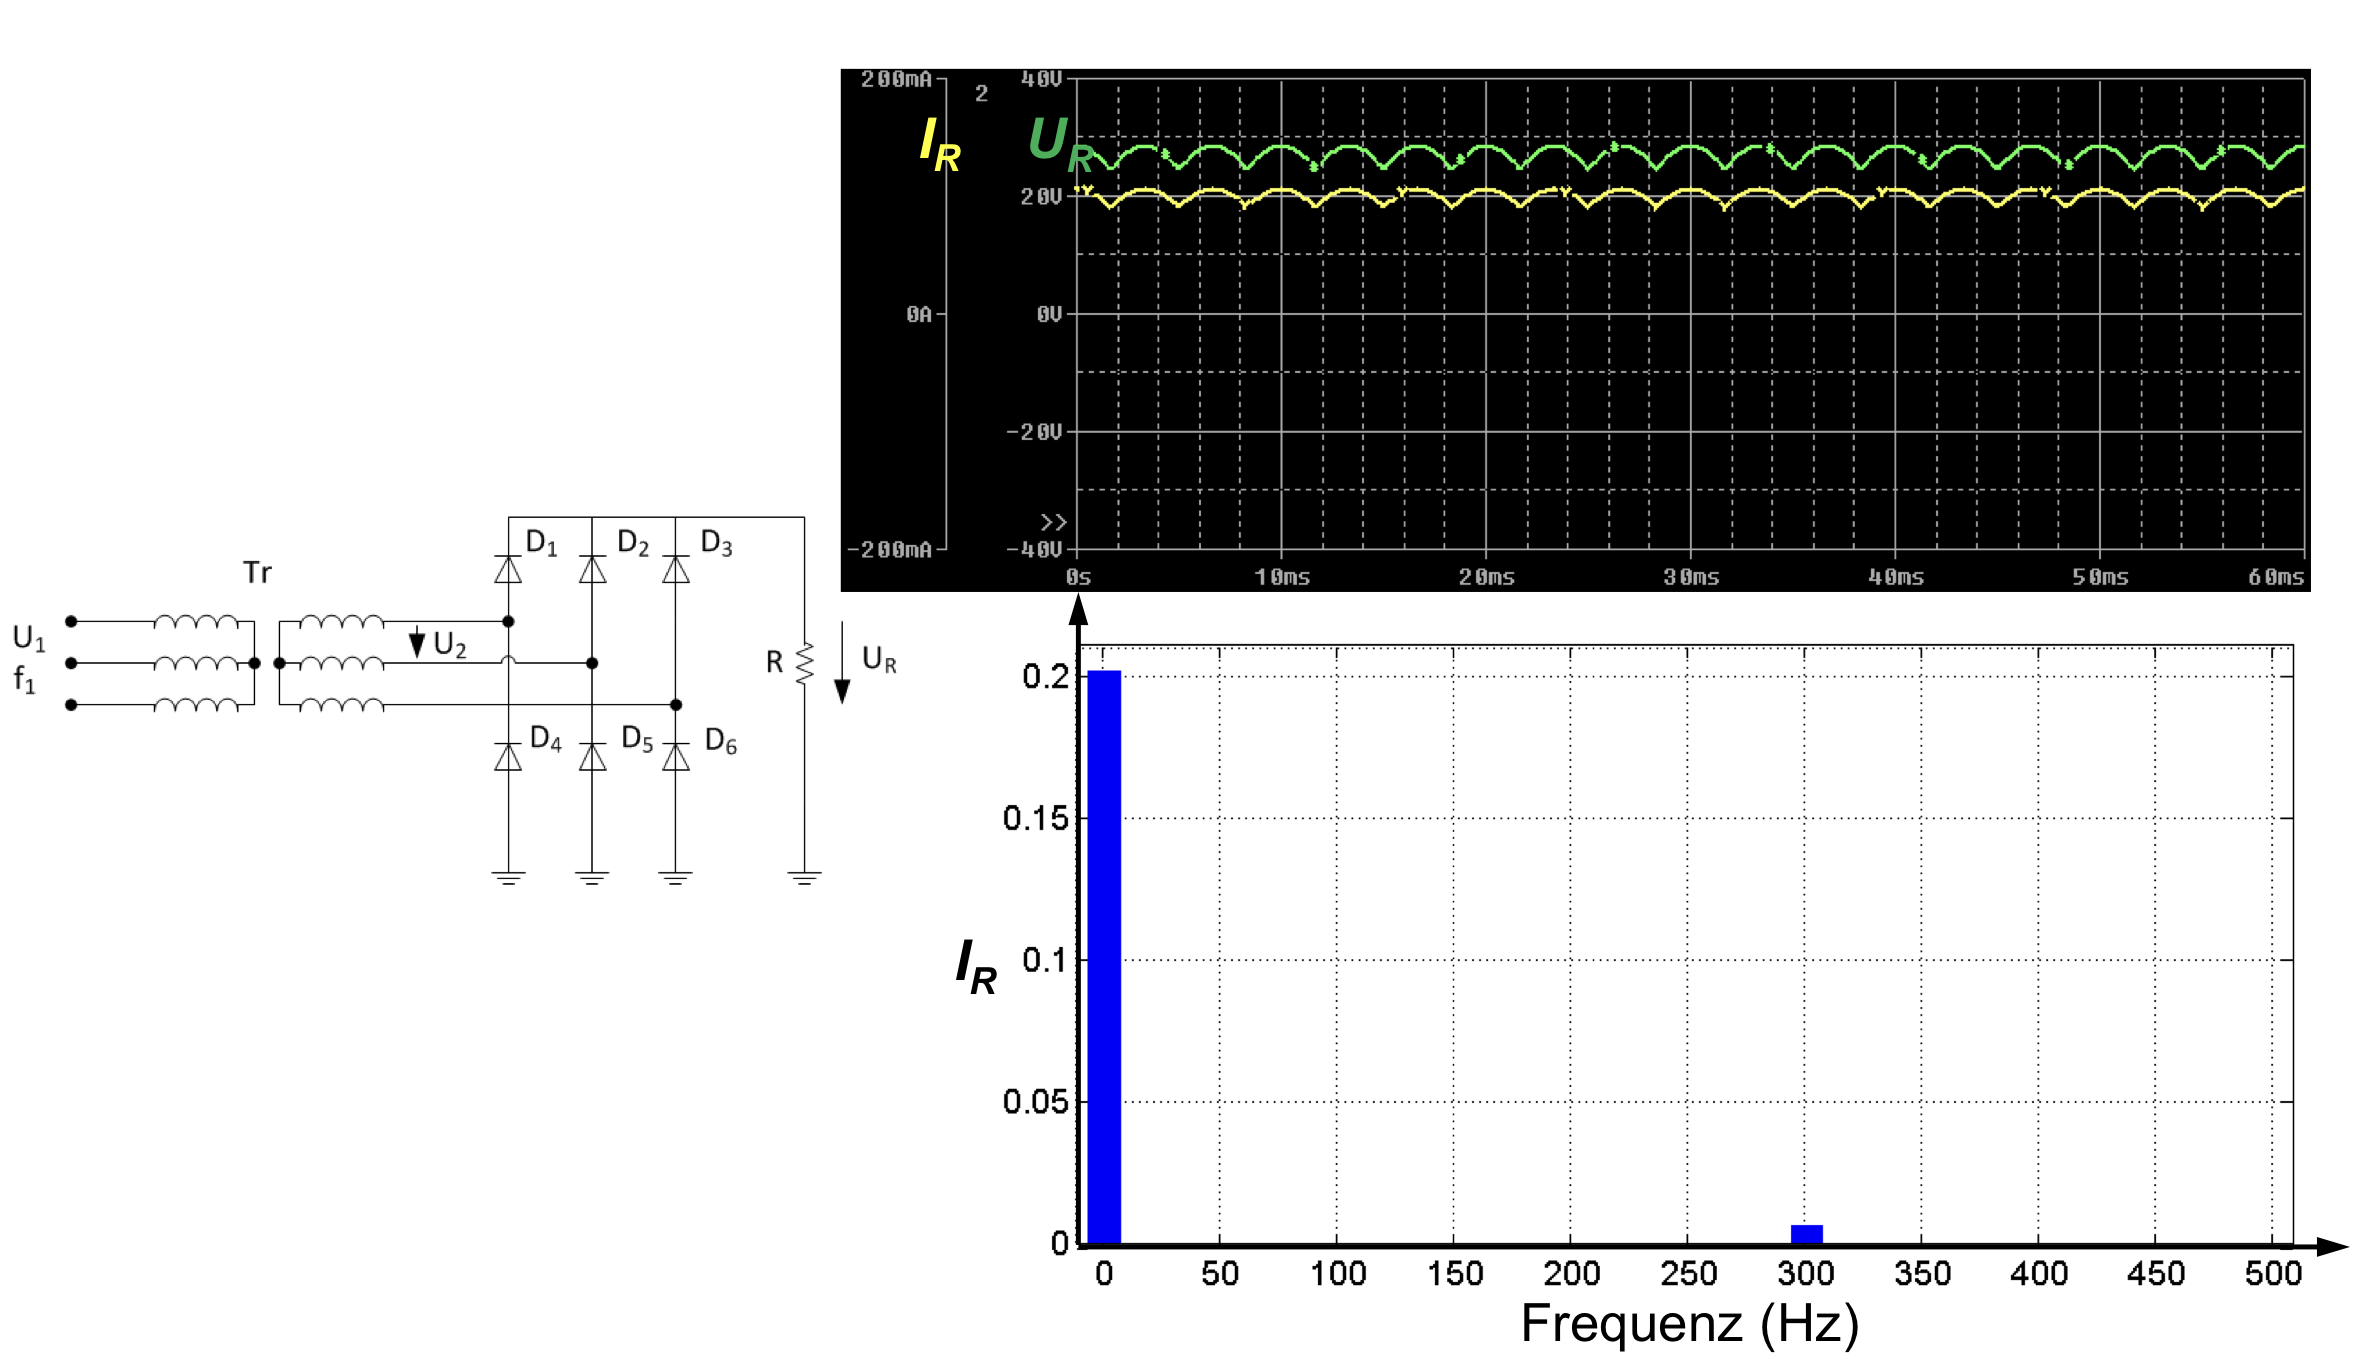
\includegraphics[width=0.85\linewidth]{images/B6U_verlauf.png}
\end{center}

\subsection{B6C: Gesteuerter Dreiphasen-Brückengleichrichter}

% --- bestehende Grafik: Schaltung ---
\begin{center}
    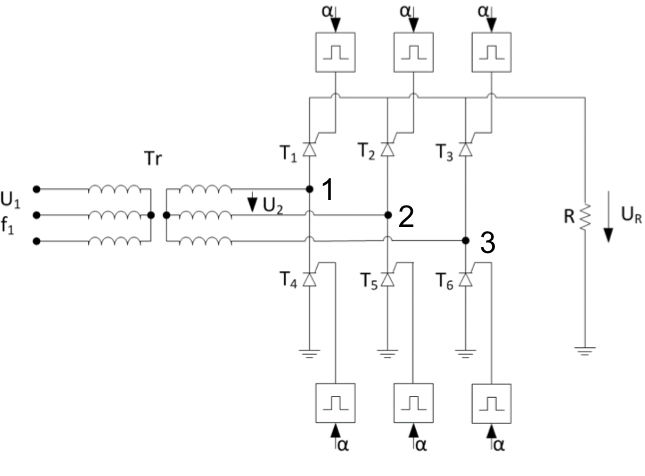
\includegraphics[width=0.65\linewidth]{images/B6C.png}
\end{center}

Der gesteuerte Dreiphasen-Brückengleichrichter ersetzt die Dioden durch Thyristoren.
Der Leitbeginn jedes Ventils wird über den Zündwinkel $\alpha$ gesteuert.

Eingangsspannungen:
\[
u_{ab}(t),\; u_{bc}(t),\; u_{ca}(t)
\]
mit:
\begin{itemize}
\item $U_{LL}$: Effektivwert der Leiterspannung,
\item $\hat U_{LL} = \sqrt{2} U_{LL}$: Scheitelwert der Leiterspannung,
\item $\omega = 2\pi f$: Kreisfrequenz,
\item $f$: Netzfrequenz.
\end{itemize}

Leitbedingung:
\[
\boxed{\omega t \ge \alpha}
\]

Momentane Ausgangsspannung:
\[
u_d(t) = u_{k\ell}(t)
\]
mit:
\begin{itemize}
\item $u_{k\ell}(t)$: jeweils aktive Leiterspannung des gerade leitenden Ventilpaares.
\end{itemize}

Mittelwert der Gleichspannung (ideal, ohne Überlappung):
\[
\cbl{\overline{u_d}
= \frac{3\sqrt{2}}{\pi} U_{LL} \cos\alpha}
\]

Stellbereich:
\[
0 \le \alpha \le \pi
\]

Grenzfälle:
\[
\alpha = 0 \Rightarrow \overline{u_d} = \frac{3\sqrt{2}}{\pi} U_{LL}
\]
\[
\alpha = \frac{\pi}{2} \Rightarrow \overline{u_d} = 0
\]
\[
\alpha > \frac{\pi}{2} \Rightarrow \overline{u_d} < 0 \quad \text{(Rückspeisebetrieb möglich)}
\]

Mittelwert des Gleichstroms bei ohmscher Last $R$:
\[
\cbl{I_d = \frac{\overline{u_d}}{R}
= \frac{3\sqrt{2}}{\pi}\frac{U_{LL}}{R}\cos\alpha}
\]

Effektivwert der Gleichspannung:
\[
\cbl{U_{d,\mathrm{RMS}}
= \sqrt{\frac{1}{2\pi}\int_0^{2\pi} u_d^2(\gamma)\, d\gamma}}
\]

Leistungsaufnahme an ohmscher Last:
\[
\cbl{P = R I_{d,\mathrm{RMS}}^2}
\]

Leistungsfaktor bei ohmscher Last:
\[
\cbl{\lambda = \frac{P}{\sqrt{3} U_{LL} I_{L,\mathrm{RMS}}}}
\]
mit:
\begin{itemize}
\item $I_{L,\mathrm{RMS}}$: Effektivwert des Leiterstroms.
\end{itemize}

Eigenschaften:
\begin{itemize}
\item Stellbare Gleichspannung über den Zündwinkel $\alpha$.
\item Mittelwert proportional zu $\cos\alpha$.
\item Rückspeisebetrieb für $\alpha > 90^\circ$.
\item Wichtigster gesteuerter Industrie-Gleichrichter.
\end{itemize}

% --- bestehende Grafik: Zeitverlauf ---
\begin{center}
    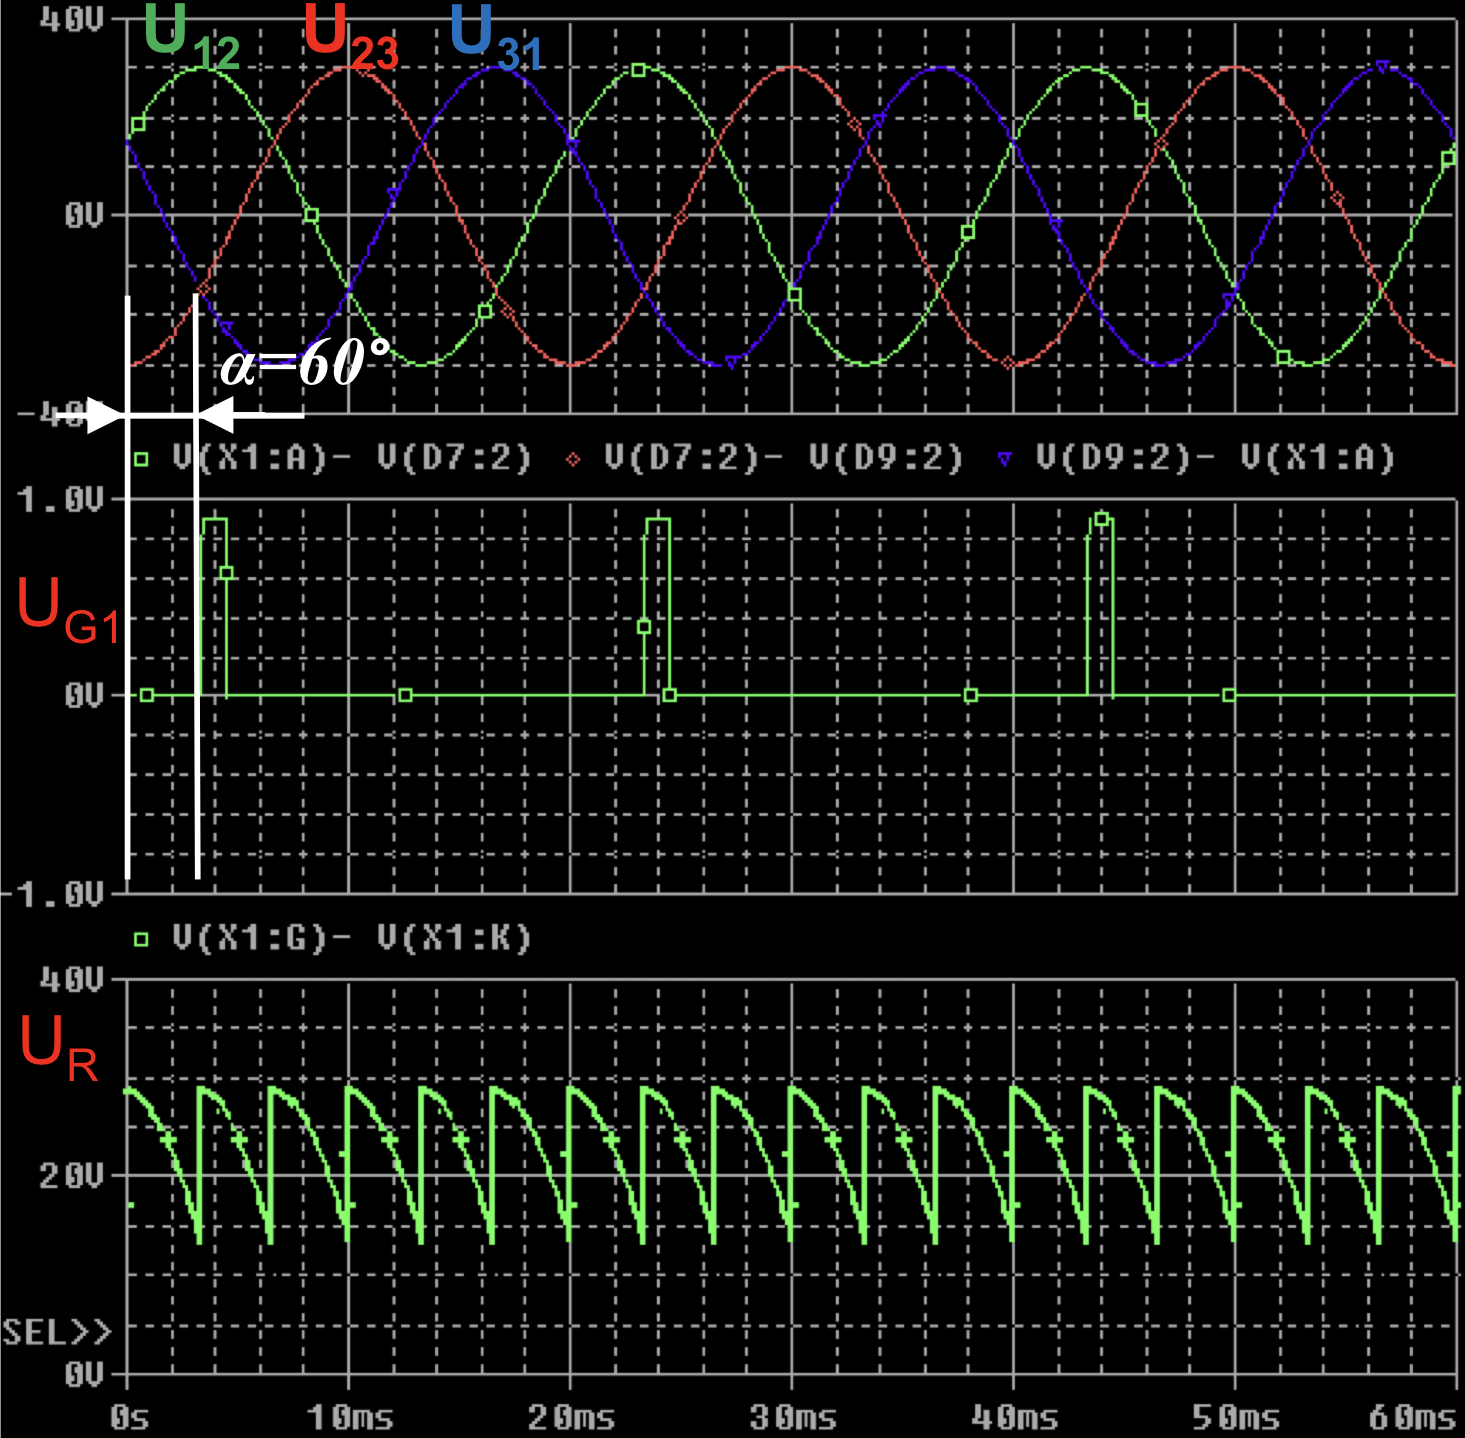
\includegraphics[width=0.85\linewidth]{images/B6C_Verlauf.png}
\end{center}

        \section{Wechselstromschalter, Wechselstromsteller und Gleichstromsteller}

Leistungselektronische Stellglieder lassen sich in Wechselstromschalter,
Wechselstromsteller und Gleichstromsteller einteilen.
Sie unterscheiden sich durch die Art der Spannung, die Stellgrösse
und die verwendete Schaltfrequenz.

% =========================================================
\subsection{Wechselstromschalter}

% --- bestehende Grafik ---
Wechselstromschalter mit bidirektionalem Ventil
\begin{center}
    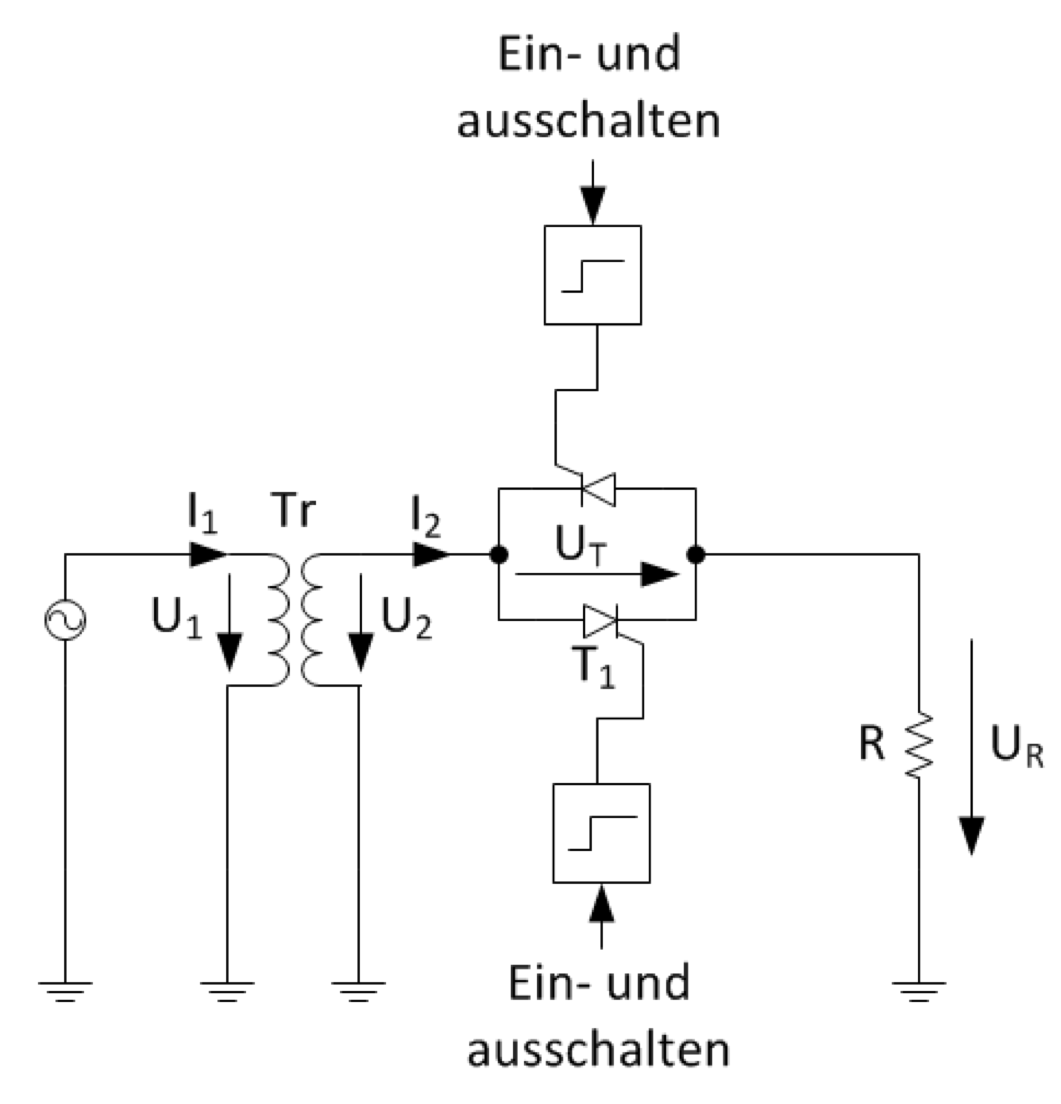
\includegraphics[width=0.85\linewidth]{images/Wechselstromschalter.png}
\end{center}

Ein Wechselstromschalter dient ausschließlich zum Ein- und Ausschalten einer Wechselspannung.
Er verändert weder die Spannungsform noch den Effektivwert, sondern schaltet die Last lediglich zu oder ab.
Die Steuerung erfolgt binär, ohne Stellfunktion.
Typische Anwendungen sind Netzschütze, Relais und einfache Netzschalter.
Wechselstromschalter sind keine Steller.

Schaltgleichung:
\[
u_L(t)=
\begin{cases}
u_s(t), & \text{Schalter geschlossen},\\
0, & \text{Schalter offen}.
\end{cases}
\]

mit:
\begin{itemize}
\item $u_s(t)$: Eingangsspannung,
\item $u_L(t)$: Lastspannung.
\end{itemize}

% =========================================================
\subsection{Wechselstromsteller (Phasenanschnittsteller)}

% --- bestehende Grafik ---
Phasenanschnittsteuerung beim Wechselstromsteller
\begin{center}
    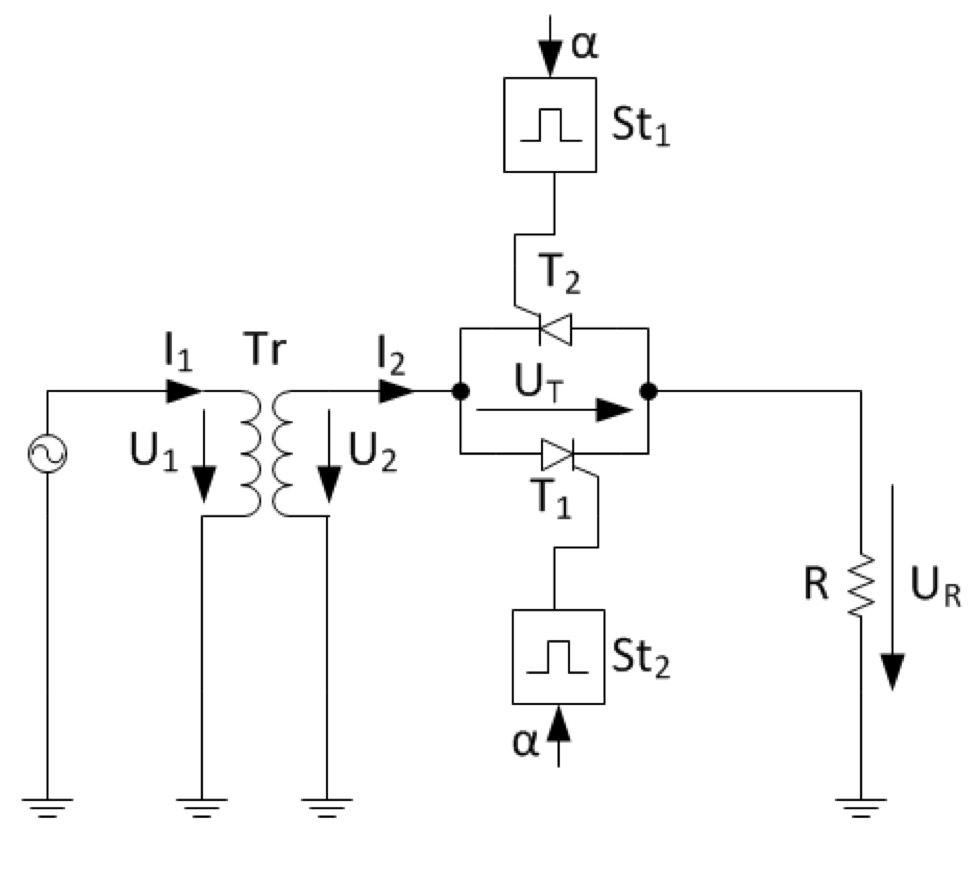
\includegraphics[width=0.85\linewidth]{images/Wechselstromsteller.png}
\end{center}

Ein Wechselstromsteller erzeugt aus einer konstanten Wechselspannung eine stellbare Wechselspannung
durch Phasenanschnittsteuerung.
Der Leitbeginn wird über den Zündwinkel $\alpha$ festgelegt.
Die Ausgangsspannung ist nicht sinusförmig und enthält starke Oberschwingungen.
Die Regelung erfolgt mit Netzfrequenz.
Typische Anwendungen sind Lichtdimmer und Heizleistungssteller.

Eingangsspannung:
\[
u_s(t)=\hat U \sin(\omega t)
\]

mit:
\begin{itemize}
\item $\hat U$: Scheitelwert,
\item $U_s=\hat U/\sqrt{2}$: Effektivwert der Eingangsspannung,
\item $\omega=2\pi f$: Kreisfrequenz,
\item $f$: Netzfrequenz.
\end{itemize}

Momentane Ausgangsspannung:
\[
u(t)=
\begin{cases}
\hat U\sin(\omega t), & \omega t \ge \alpha,\\
0, & \omega t < \alpha.
\end{cases}
\]

\paragraph{R-Last}

Effektivwert:
\[
\boxed{
U_{\mathrm{RMS}}(\alpha)
=U_s\sqrt{\frac{1}{\pi}\int_{\alpha}^{\pi}\sin^2\theta\,d\theta}
}
\]

Geschlossene Form:
\[
\boxed{
U_{\mathrm{RMS}}(\alpha)
=U_s\sqrt{\frac{1}{2\pi}\left(\pi-\alpha+\frac{1}{2}\sin 2\alpha\right)}
}
\]

Strom:
\[
\boxed{I_{\mathrm{RMS}}(\alpha)=\frac{U_{\mathrm{RMS}}(\alpha)}{R}}
\]

Wirkleistung:
\[
\boxed{P(\alpha)=\frac{U_{\mathrm{RMS}}^2(\alpha)}{R}}
\]

Mittelwert der Ausgangsspannung:
\[
\boxed{
\overline{u}(\alpha)=\frac{1}{2\pi}\int_{\alpha}^{\pi}\hat U\sin\theta\,d\theta
=\frac{\hat U}{2\pi}(1+\cos\alpha)
}
\]

\paragraph{R--L-Last}

Differentialgleichung im Leitintervall:
\[
L\frac{di}{dt}+Ri=\hat U\sin(\omega t)
\]

Allgemeine Lösung:
\[
\boxed{
i(t)=C e^{-t/\tau}+\frac{\hat U}{Z}\sin(\omega t-\varphi)
}
\]

mit:
\[
\tau=\frac{L}{R},\qquad
Z=\sqrt{R^2+(\omega L)^2},\qquad
\tan\varphi=\frac{\omega L}{R}
\]

Löschwinkel:
\[
\boxed{i(\beta)=0}
\]

Leitbedingung:
\[
\boxed{\alpha<\beta}
\]

Eigenschaften:
\begin{itemize}
\item Stellgrösse: Zündwinkel $\alpha$,
\item Nichtsinusförmige Spannung und Strom,
\item Starke Netzstromharmonische,
\item Schlechter Leistungsfaktor bei kleinem $\alpha$.
\end{itemize}

% =========================================================
\subsection{Gleichstromsteller (Chopper)}

Ein Gleichstromsteller wandelt eine konstante Gleichspannung $U_{DC}$
in eine stufenlos einstellbare Gleichspannung $u_d$
durch schnelles periodisches Ein- und Ausschalten eines Halbleiterschalters.
Die Stellgrösse ist der Tastgrad $d$.
Der Schalter arbeitet mit hoher Schaltfrequenz $f_s$.
Im kontinuierlichen Betrieb entspricht der Gleichstromsteller einem Buck-Wandler.
Er ist das Standard-Stellglied für Gleichstromantriebe.

% -------------------------------------------------
\subsubsection{Grundgrössen und Definitionen}

Tastgrad:
\[
\boxed{d=\frac{t_{\mathrm{on}}}{T_s}}, 
\qquad
T_s=\text{Schaltperiode}, 
\qquad
f_s=\frac{1}{T_s}
\]

Mittelwert der Ausgangsspannung (CCM):
\[
\boxed{u_d=d\,U_{DC}}
\]

Effektivwert der Ausgangsspannung (ideales PWM-Rechteck):
\[
\boxed{U_{d,\mathrm{RMS}}=U_{DC}\sqrt{d}}
\]

mit:
\begin{itemize}
\item $U_{DC}$: Eingangsgleichspannung,
\item $u_d$: mittlere Ausgangsspannung,
\item $U_{d,\mathrm{RMS}}$: Effektivwert der Ausgangsspannung,
\item $t_{\mathrm{on}}$: Einschaltzeit,
\item $T_s$: Schaltperiode,
\item $f_s$: Schaltfrequenz.
\end{itemize}

Ausgangsleistung (ideal):
\[
\boxed{P_{\mathrm{out}}=u_d\,I_d}
\]

% -------------------------------------------------
\subsubsection{R--L-Last im Zeitbereich}

Lastgleichung:
\[
L\frac{di}{dt}+Ri=u_d(t)
\]

Zeitkonstante:
\[
\boxed{\tau=\frac{L}{R}}
\]

\paragraph{EIN-Phase ($0<t<t_{\mathrm{on}}$)}

\[
L\frac{di}{dt}+Ri=U_{DC}
\]

\[
\boxed{
i(t)=\frac{U_{DC}}{R}
+\left(i_{\min}-\frac{U_{DC}}{R}\right)e^{-t/\tau}
}
\]

\paragraph{AUS-Phase ($t_{\mathrm{on}}<t<T_s$)}

\[
L\frac{di}{dt}+Ri=0
\]

\[
\boxed{
i(t)=i_{\max}e^{-t/\tau}
}
\]

Periodenbedingung:
\[
\boxed{i_{\min}=i_{\max}e^{-T_a/\tau}}, 
\qquad T_a=T_s-t_{\mathrm{on}}
\]

% -------------------------------------------------
\subsubsection{Induktorspannung und Mittelwertbedingung}

Induktorspannung:
\[
u_L(t)=L\frac{di}{dt}
\]

Stationärer Betrieb:
\[
\boxed{\overline{u_L}=0}
\]

Daraus folgt direkt:
\[
\boxed{u_d=d\,U_{DC}}
\]

Dies ist die fundamentale Mittelwertbedingung des Gleichstromstellers.

% -------------------------------------------------
\subsubsection{Stromrippel und Betriebsarten}

Stromrippel:
\[
\boxed{\Delta i=i_{\max}-i_{\min}}
\]

Während EIN:
\[
\boxed{
\Delta i_{\mathrm{on}}\approx\frac{(U_{DC}-u_d)}{L}\,dT_s
}
\]

Während AUS:
\[
\boxed{
\Delta i_{\mathrm{off}}\approx\frac{u_d}{L}\,(1-d)T_s
}
\]

Stationär:
\[
\boxed{\Delta i=\Delta i_{\mathrm{on}}=\Delta i_{\mathrm{off}}}
\]

\paragraph{Grenzbetrieb CCM/DCM}

Grenzstrom:
\[
\boxed{I_{d,\mathrm{gr}}=\frac{\Delta i}{2}}
\]

Grenzinduktivität:
\[
\boxed{
L_{\min}=\frac{(1-d)R}{2f_s}
}
\]

\begin{itemize}
\item $L>L_{\min}$: kontinuierlicher Betrieb (CCM),
\item $L<L_{\min}$: diskontinuierlicher Betrieb (DCM),
\item DCM: $u_d=dU_{DC}$ gilt nicht mehr exakt.
\end{itemize}

% -------------------------------------------------
\subsubsection{Schalter- und Diodenbelastung}

Schalterstrom:
\[
i_S(t)=
\begin{cases}
i(t), & 0<t<t_{\mathrm{on}},\\
0, & t_{\mathrm{on}}<t<T_s
\end{cases}
\]

Diodenstrom:
\[
i_D(t)=
\begin{cases}
0, & 0<t<t_{\mathrm{on}},\\
i(t), & t_{\mathrm{on}}<t<T_s
\end{cases}
\]

Mittelwerte:
\[
\boxed{
I_{S,\mathrm{avg}}=d\,I_d,
\qquad
I_{D,\mathrm{avg}}=(1-d)\,I_d
}
\]

Effektivwerte (kleiner Rippel):
\[
\boxed{
I_{S,\mathrm{RMS}}\approx\sqrt{d}\,I_d,
\qquad
I_{D,\mathrm{RMS}}\approx\sqrt{1-d}\,I_d
}
\]

% =========================================================
\subsubsection{Einquadrantensteller (1Q)}

% --- bestehende Grafik ---
\begin{center}
    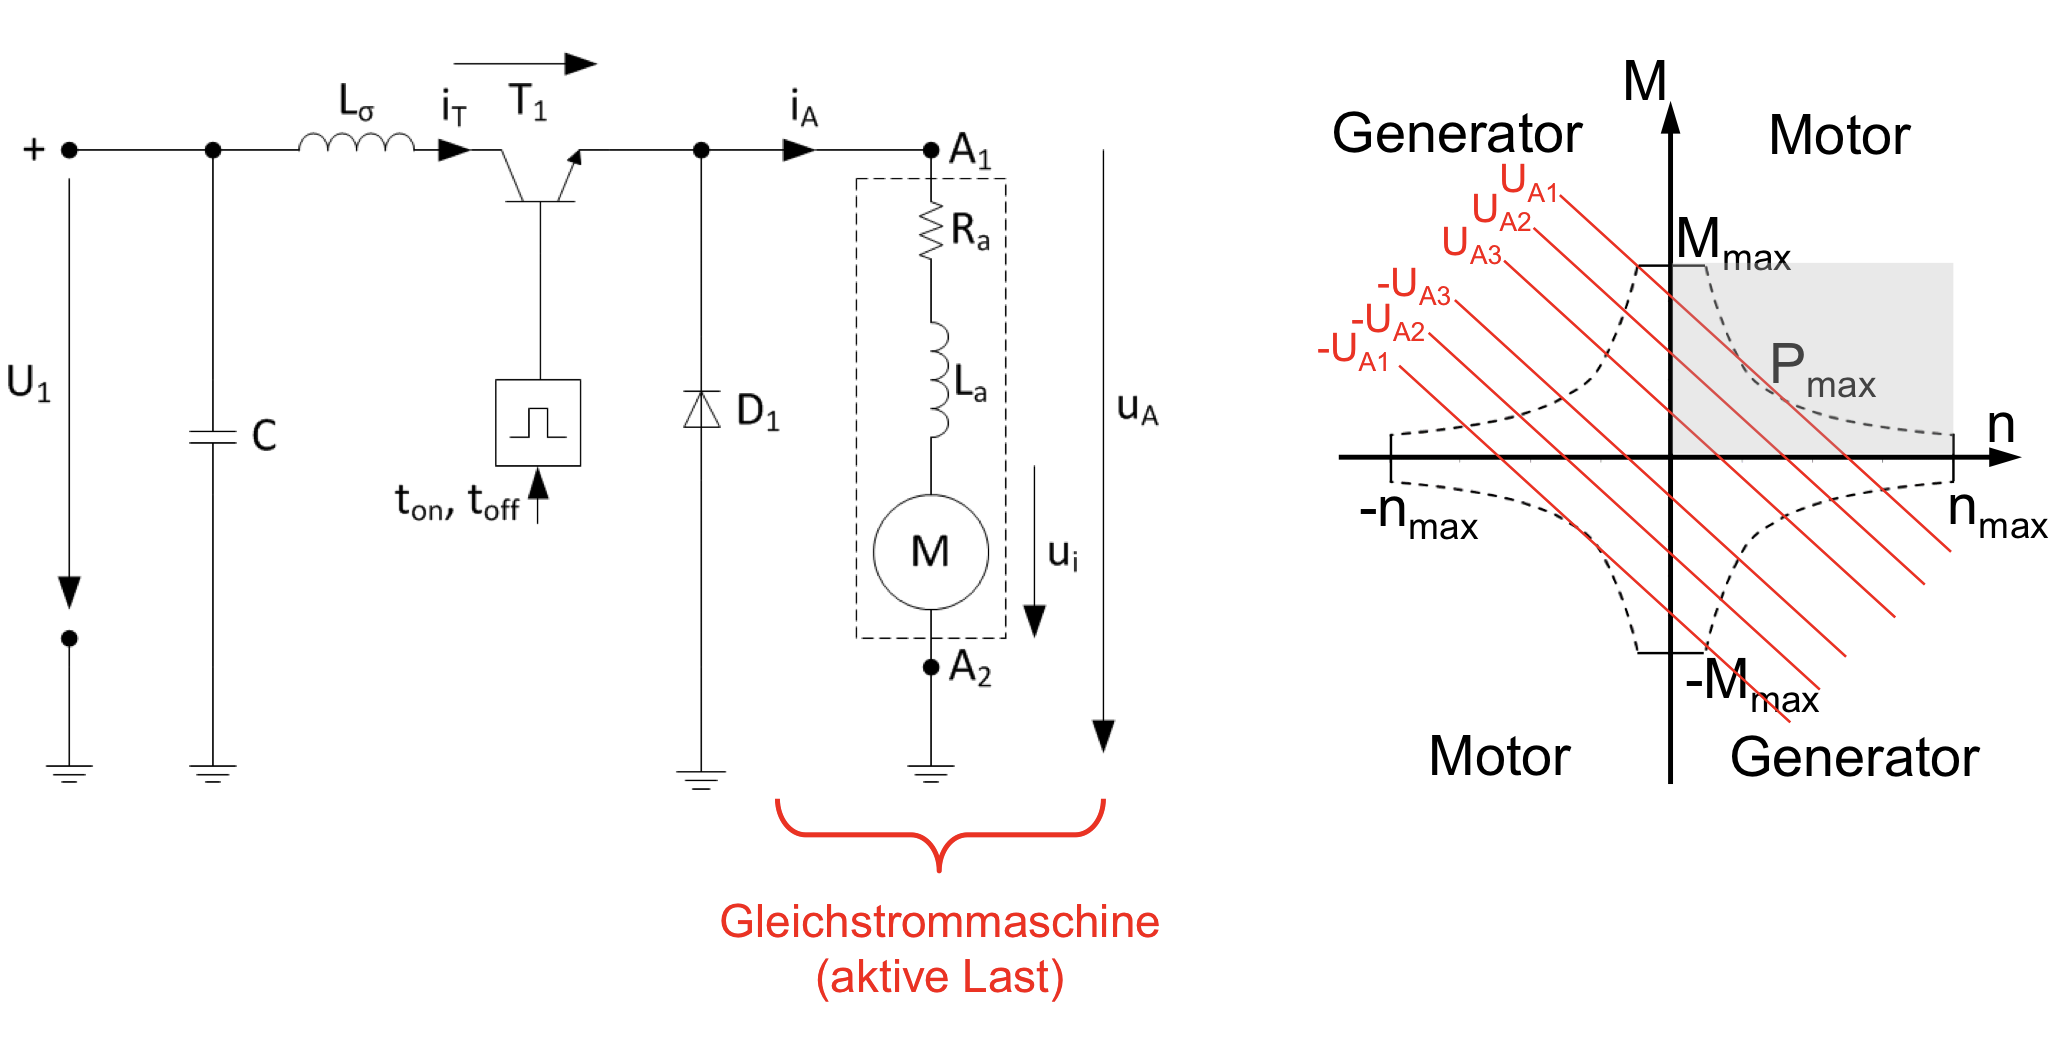
\includegraphics[width=0.85\linewidth]{images/Gleichstromsteller1Q.png}
\end{center}

Der Einquadrantensteller erlaubt nur positive Spannung und positiven Strom.
Er arbeitet ausschließlich im Motorbetrieb vorwärts.
Energie kann nur von der Quelle zur Last fliessen.
Eine Rückspeisung ist nicht möglich.
Dies ist die einfachste und am häufigsten eingesetzte Chopper-Topologie.

Betriebsbereich:
\[
\boxed{u_d\ge 0,\qquad i_d\ge 0,\qquad P=u_d i_d>0}
\]

Spannungssteuerung:
\[
\boxed{u_d=d\,U_{DC}}
\]

% =========================================================
\subsubsection{Zweiquadrantensteller (2Q)}

% --- bestehende Grafik ---
\begin{center}
    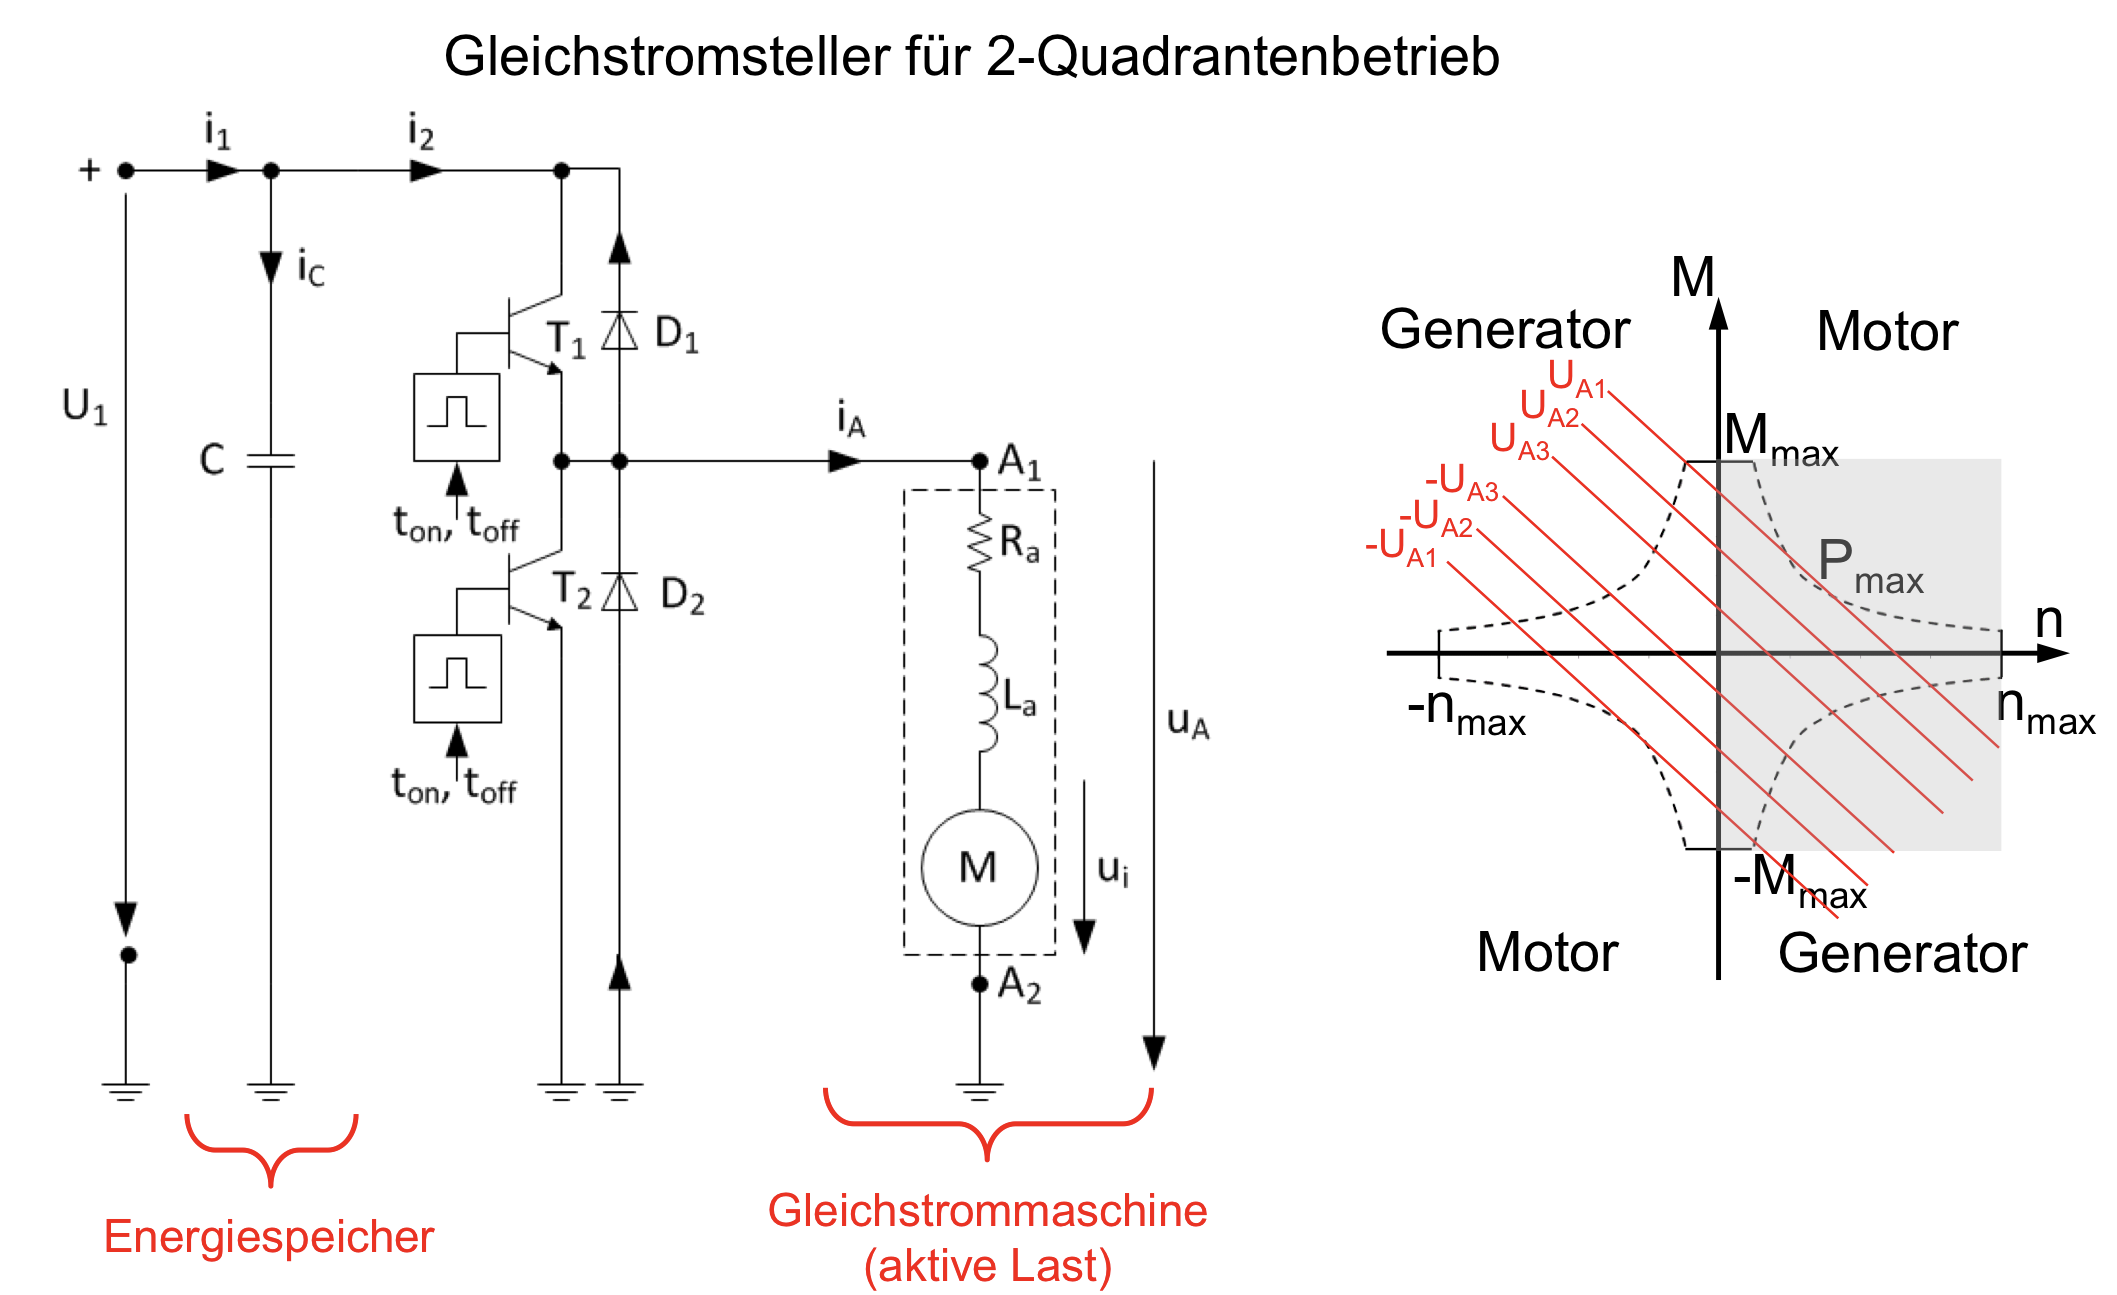
\includegraphics[width=0.85\linewidth]{images/Gleichstromsteller2Q.png}
\end{center}

Der Zweiquadrantensteller erlaubt positiven Spannungsbetrieb bei wechselndem Strom.
Er kann sowohl Motorbetrieb als auch generatorischen Bremsbetrieb realisieren.
Im generatorischen Betrieb wird Energie zur Quelle zurückgespeist.
Die Drehrichtung bleibt gleich, das Drehmoment kann sein Vorzeichen wechseln.
Diese Struktur wird für geregelte Bremsvorgänge verwendet.

Betriebsbereich:
\[
\boxed{u_d\ge 0,\qquad i_d \text{ vorzeichenwechselnd}}
\]

Leistung:
\[
\boxed{P=u_d i_d}
\]

\[
P>0 \Rightarrow \text{Motorbetrieb},
\qquad
P<0 \Rightarrow \text{Rekuperation}
\]

% =========================================================
\subsubsection{Vierquadrantensteller (4Q)}

% --- bestehende Grafik ---
\begin{center}
    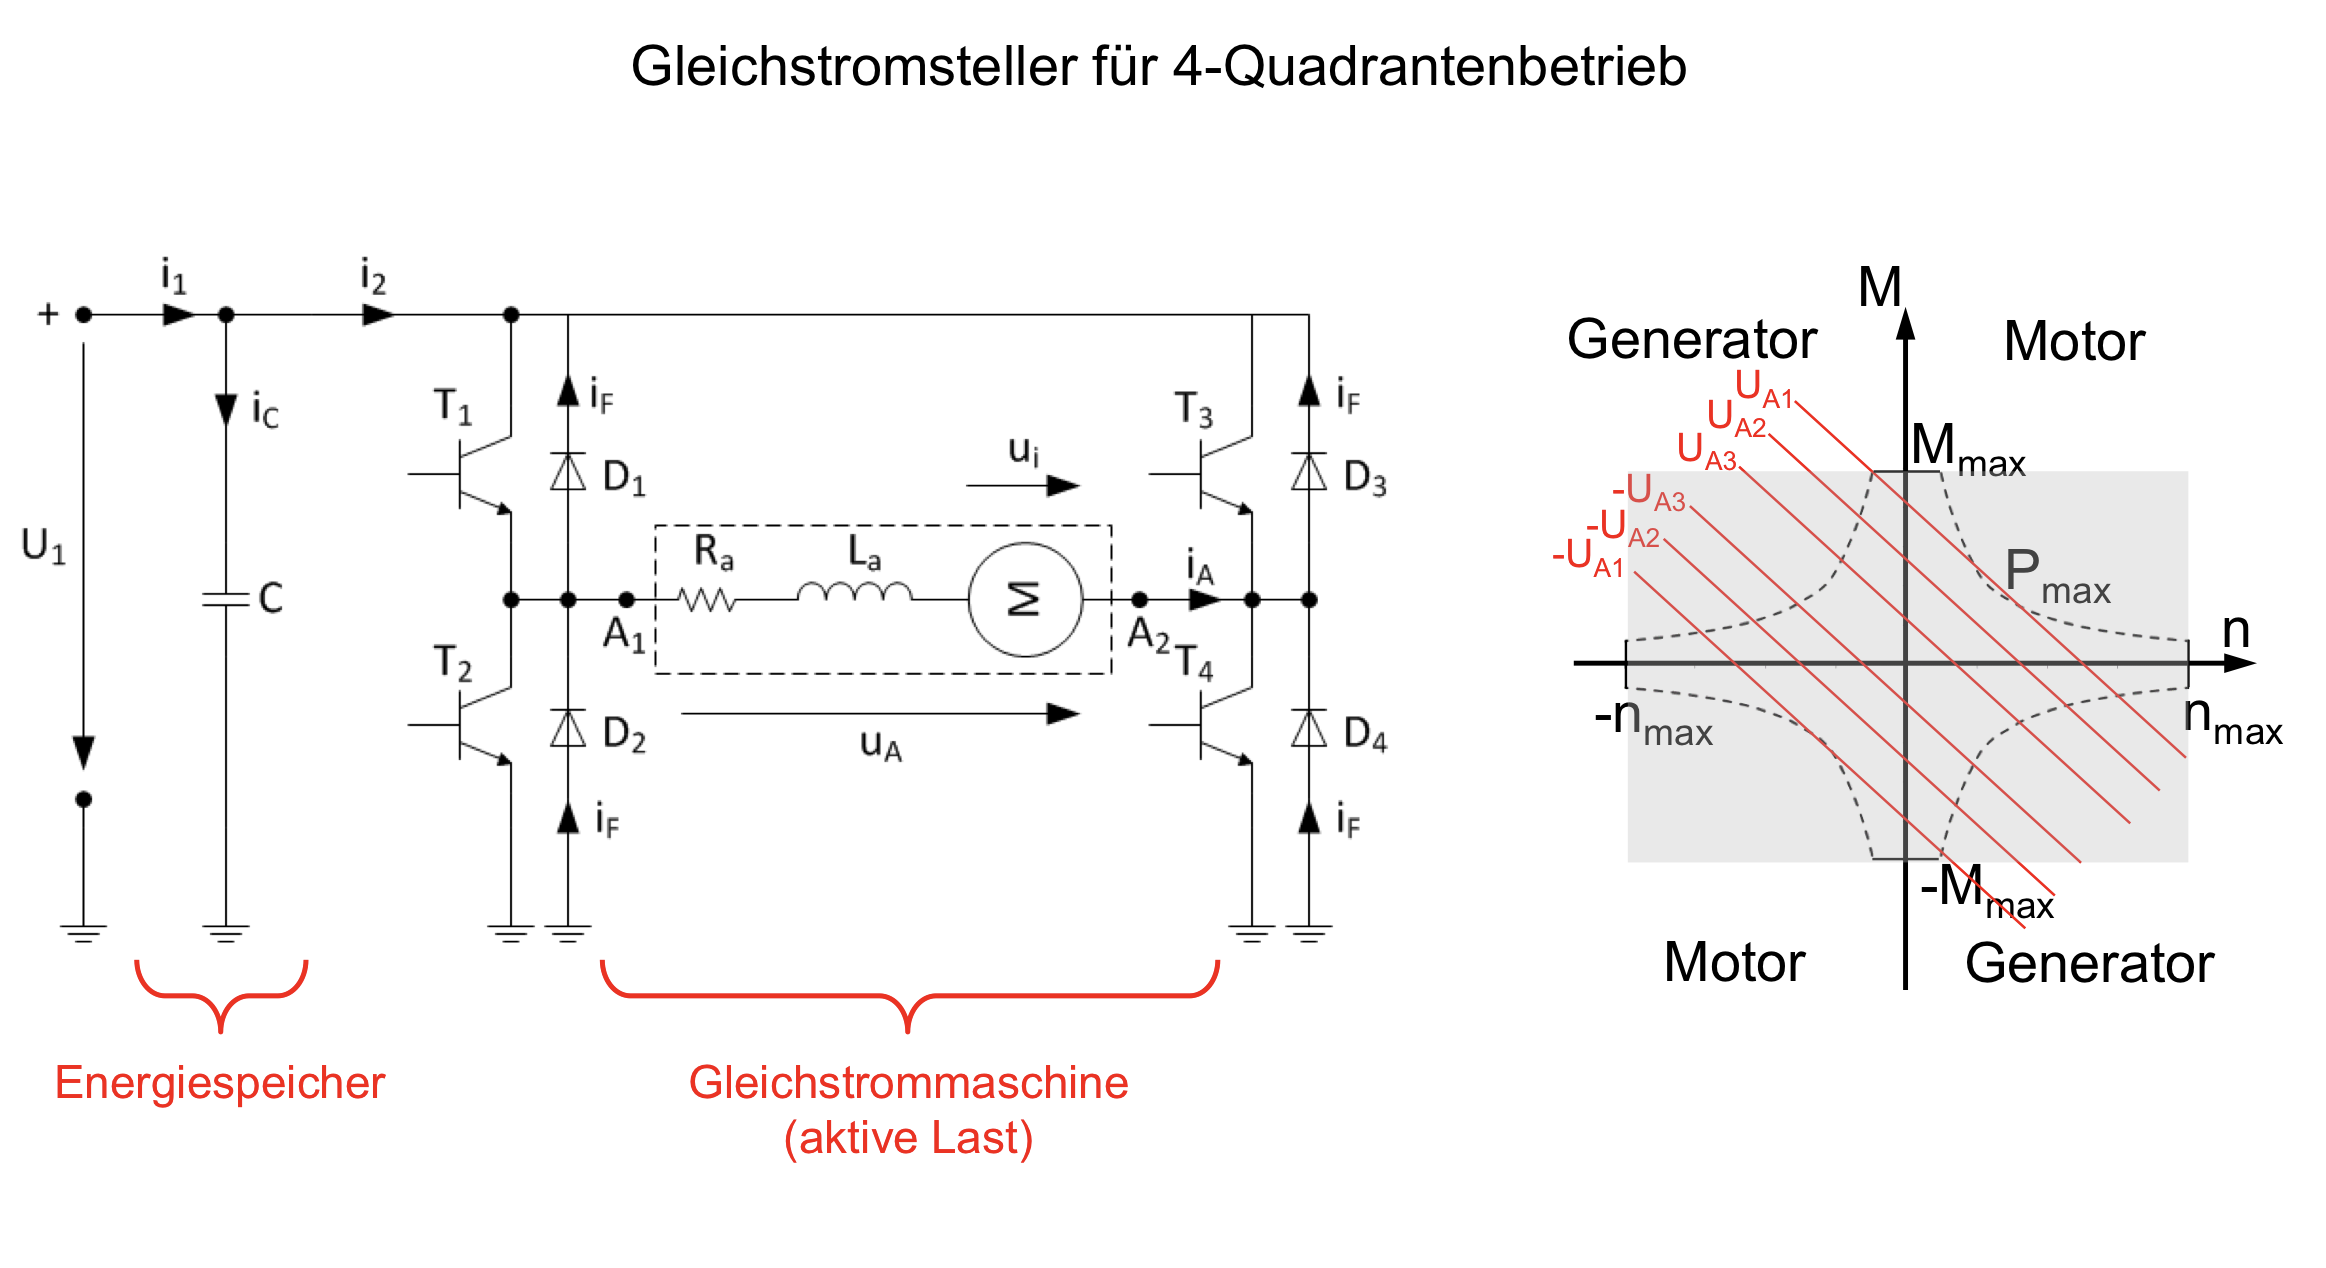
\includegraphics[width=0.85\linewidth]{images/Gleichstromsteller4Q.png}
\end{center}

Der Vierquadrantensteller erlaubt Spannungs- und Stromumkehr.
Er ermöglicht Motor- und Generatorbetrieb in beiden Drehrichtungen.
Damit sind Vorwärts- und Rückwärtslauf sowie Bremsbetrieb möglich.
Diese Topologie ist die vollständigste Form des Gleichstromstellers.
Sie wird in Reversierantrieben und Positioniersystemen eingesetzt.

Betriebsbereich:
\[
\boxed{
u_d \text{ vorzeichenwechselnd},
\qquad
i_d \text{ vorzeichenwechselnd}
}
\]

Quadranten:
\[
\begin{aligned}
\text{I:} &\; u>0,\; i>0 \quad \text{Motor vorwärts},\\
\text{II:} &\; u<0,\; i>0 \quad \text{Generator vorwärts},\\
\text{III:} &\; u<0,\; i<0 \quad \text{Motor rückwärts},\\
\text{IV:} &\; u>0,\; i<0 \quad \text{Generator rückwärts}.
\end{aligned}
\]

% -------------------------------------------------
\subsubsection{Bezug zur Gleichstrommaschine}

Ankergleichung:
\[
\boxed{u_d=R_a i_a+k\Phi\omega}
\]

Drehmoment:
\[
\boxed{M=k\Phi i_a}
\]

Drehzahl:
\[
\boxed{\omega=\frac{u_d-R_a i_a}{k\Phi}
\approx \frac{u_d}{k\Phi}}
\]

Eigenschaften:
\begin{itemize}
\item $d\uparrow \Rightarrow u_d\uparrow \Rightarrow \omega\uparrow$,
\item $d\downarrow \Rightarrow u_d\downarrow \Rightarrow \omega\downarrow$,
\item Gleichstromsteller ist das Standard-Stellglied für DC-Antriebe.
\end{itemize}


% =========================================================
\subsection{Vergleich AC-Steller -- DC-Steller}

\begin{center}
\begin{tabular}{l|c|c}
 & AC-Steller & DC-Steller \\ \hline
Spannung & Wechselspannung & Gleichspannung \\
Stellgrösse & Zündwinkel $\alpha$ & Tastgrad $d$ \\
Schaltfrequenz & Netzfrequenz & \cbl{hoch} \\
Last & R, R--L & \cbl{R--L} \\
Hauptanwendung & Heizung, Licht & \cbl{Antriebe} \\
\end{tabular}
\end{center}

        \section{Gleichstrommaschine im Umrichterbetrieb}

Diese Section behandelt die \textbf{Gleichstrommaschine} als Last und Antrieb im Zusammenspiel mit
\textbf{Gleichrichtern} und \textbf{Gleichstromstellern}.
Sie ist zentral für die Analyse von \textbf{Drehzahl}, \textbf{Drehmoment}, \textbf{Stabilität} und
für das Verständnis der \textbf{Kennlinien $M$--$n$} sowie des \textbf{Quadrantenbetriebs}.

\smallskip

\textbf{Zielbild:}
\begin{itemize}
    \item Grundgleichungen der Gleichstrommaschine kennen (elektrisch und mechanisch)
    \item Zusammenhang zwischen Spannung, Strom, Drehzahl und Drehmoment verstehen
    \item Einfluss der Ankerspannung und des Erregerflusses auf die Kennlinie analysieren
    \item Arbeitspunkt bestimmen und Stabilität beurteilen
    \item Betrieb mit 1Q-, 2Q- und 4Q-Stellern (Motor/Generator) einordnen
\end{itemize}

\subsection*{Konvention für Maschinenkonstanten}

Zur Vereinheitlichung der Notation wird im Folgenden definiert:

\[
\boxed{k\Phi \;\equiv\; \Psi}
\]

mit:
\begin{itemize}
    \item $\Phi$: Erregerfluss,
    \item $k$: Maschinenkonstante,
    \item $\Psi$: zusammengefasste Flusskonstante der Maschine.
\end{itemize}

Damit gilt einheitlich:
\[
E_i = \Psi \, \omega,
\qquad
M = \Psi \, i_a.
\]


% =========================================================
\subsection{Grundaufbau und Ersatzschaltbild}

\begin{center}
    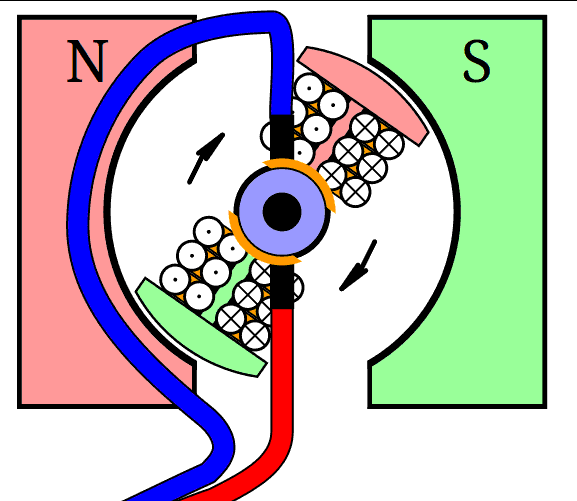
\includegraphics[width=0.85\linewidth]{images/Grundaufbau_gleistrommaschiene.png}
\end{center}

\subsubsection{Vereinfachtes Ersatzschaltbild}

\begin{center}
    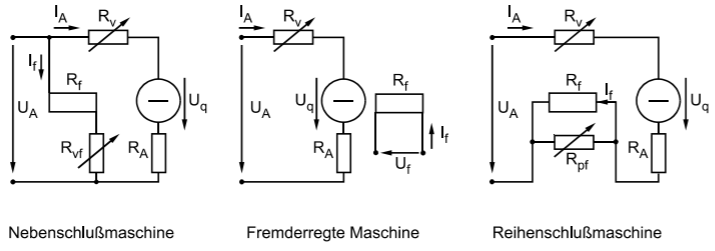
\includegraphics[width=0.85\linewidth]{images/gleichstrommasciene.png}
\end{center}

\paragraph{Elemente und Variablen}
\begin{itemize}
    \item $u_a(t)$: Ankerspannung (Ausgangsspannung des Umrichters bzw. Stellers),
    \item $i_a(t)$: Ankerstrom,
    \item $R_a$: Ankerwiderstand,
    \item $L_a$: Ankerinduktivität,
    \item $E_i(t)$: induzierte Gegenspannung (Gegen-EMK),
    \item $\omega(t)$: mechanische Winkelgeschwindigkeit,
    \item $n(t)$: Drehzahl in $\mathrm{min^{-1}}$,
    \item $M(t)$: elektromagnetisches Drehmoment.
\end{itemize}

Zusammenhang zwischen Drehzahl und Winkelgeschwindigkeit:
\[
\boxed{\omega = 2\pi \frac{n}{60}}
\]

% =========================================================
\subsection{Maschinenkonstanten und Grundzusammenhänge}

Zur einheitlichen Schreibweise wird die Maschinenkonstante $k\Phi$ verwendet.

\paragraph{Gegen-EMK}
\[
\boxed{E_i = k\Phi\,\omega}
\]

\paragraph{Drehmoment}
\[
\boxed{M = k\Phi\,i_a}
\]

mit:
\begin{itemize}
    \item $\Phi$: Erregerfluss (bzw. proportional dazu),
    \item $k$: Maschinenkonstante (Konstruktionsparameter),
    \item $k\Phi$: resultierende Konstante aus Maschine und Erregung.
\end{itemize}

\crd{\textrightarrow\ In den Grundgleichungen koppelt $k\Phi$ den elektrischen und mechanischen Teil.}

% =========================================================
\subsection{Grundgleichungen der Gleichstrommaschine}

\subsubsection{Elektrische Gleichung}

\[
\boxed{u_a(t) = R_a\, i_a(t) + L_a\, \frac{di_a(t)}{dt} + E_i(t)}
\]

Einsetzen von $E_i=k\Phi\omega$:
\[
\boxed{u_a(t) = R_a i_a(t) + L_a\frac{di_a(t)}{dt} + k\Phi\,\omega(t)}
\]

\subsubsection{Mechanische Gleichung}

\[
\boxed{J\frac{d\omega(t)}{dt} = M(t) - M_L(t) - B\,\omega(t)}
\]

mit:
\begin{itemize}
    \item $J$: Trägheitsmoment,
    \item $M_L$: Lastmoment,
    \item $B$: viskoser Reibungskoeffizient.
\end{itemize}

\subsubsection{Leistungsbeziehungen}

Elektrische Leistung:
\[
\boxed{P_{el}(t)=u_a(t)\,i_a(t)}
\]

Mechanische Leistung:
\[
\boxed{P_{mech}(t)=M(t)\,\omega(t)}
\]

Ideal (ohne Verluste) gilt näherungsweise:
\[
\boxed{P_{el}\approx P_{mech}}
\]

\crd{\textrightarrow\ Drehmoment wird direkt durch den Strom bestimmt: $M=k\Phi i_a$.}

% =========================================================
\subsection{Stationärer Betrieb}

Im stationären Betrieb gilt:
\[
\frac{di_a}{dt}=0,
\qquad
\frac{d\omega}{dt}=0
\]

Damit reduziert sich die elektrische Gleichung zu:
\[
\boxed{u_a = R_a i_a + k\Phi\,\omega}
\]

Auflösen nach der Drehzahl:
\[
\boxed{\omega=\frac{u_a-R_a i_a}{k\Phi}}
\]

\subsubsection{Strom als Funktion von Spannung und Drehzahl}

Aus $u_a=R_a i_a+k\Phi\omega$ folgt:
\[
\boxed{i_a=\frac{u_a-k\Phi\omega}{R_a}}
\]

Daraus Drehmoment als Funktion von $u_a$ und $\omega$:
\[
\boxed{M=k\Phi\,i_a=\frac{k\Phi}{R_a}\left(u_a-k\Phi\omega\right)}
\]

Interpretation:
\begin{itemize}
    \item $u_a\uparrow \Rightarrow \omega\uparrow$ (bei gleicher Last),
    \item $M_L\uparrow \Rightarrow i_a\uparrow \Rightarrow \omega\downarrow$.
\end{itemize}

% =========================================================
\subsection{Spezialfall: Leerlaufbetrieb}

Leerlauf bedeutet: sehr kleines Lastmoment $M_L \approx 0$ und damit sehr kleiner Ankerstrom $i_a \approx 0$.
Im idealen Leerlauf (ohne Reibung) folgt aus $M = i_a \Psi$ direkt $i_a \approx 0$.
Damit gilt stationär aus $u_a = R_a i_a + \omega \Psi$ näherungsweise:

\[
\boxed{i_{a,0} \approx 0}
\]
\[
\boxed{\omega_0 \approx \frac{u_a}{\Psi}}
\]

Mit Reibung $B$ ergibt sich im stationären Betrieb näherungsweise:
\[
M \approx B\omega
\quad\Rightarrow\quad
i_a \approx \frac{B\omega}{\Psi}
\]
und damit:
\[
\boxed{u_a \approx R_a\frac{B\omega}{\Psi} + \omega\Psi}
\]

mit:
\begin{itemize}
\item $M_L$: Lastmoment,
\item $B$: Reibungskoeffizient,
\item $i_{a,0}$: Leerlaufstrom,
\item $\omega_0$: Leerlaufdrehzahl.
\end{itemize}
\subsection{Spezialfall: Blockierfall (gesperrter Rotor)}

Im Blockierfall ist der Rotor mechanisch gesperrt:
\[
\boxed{\omega = 0}
\]

Damit ist die Gegen-EMK null:
\[
\boxed{E_i = \omega\Psi = 0}
\]

Die elektrische Gleichung reduziert sich im stationären Fall ($di_a/dt=0$) zu:
\[
\boxed{u_a = R_a i_a}
\quad\Rightarrow\quad
\boxed{i_{a,\mathrm{block}} = \frac{u_a}{R_a}}
\]

Das Blockiermoment ergibt sich aus $M=i_a\Psi$:
\[
\boxed{M_{\mathrm{block}} = i_{a,\mathrm{block}}\,\Psi = \frac{u_a\Psi}{R_a}}
\]

Konsequenz:
\begin{itemize}
\item Der Blockierstrom ist sehr hoch und nur durch $R_a$ begrenzt.
\item Thermische Überlast ist wahrscheinlich $\Rightarrow$ Strombegrenzung erforderlich.
\end{itemize}

mit:
\begin{itemize}
\item $i_{a,\mathrm{block}}$: Blockierstrom,
\item $M_{\mathrm{block}}$: Blockiermoment.
\end{itemize}
\subsection{M--n-Kennlinie (Drehmoment--Drehzahl-Kennlinie)}

Mit
\[
M=k\Phi i_a,
\qquad
u_a=R_a i_a+k\Phi\omega
\]

Elimination von $i_a$:
\[
i_a=\frac{M}{k\Phi}
\]

Einsetzen in $u_a=R_a i_a+k\Phi\omega$:
\[
u_a=R_a\frac{M}{k\Phi}+k\Phi\omega
\]

Auflösen nach $\omega$:
\[
\boxed{\omega=\frac{u_a}{k\Phi}-\frac{R_a}{(k\Phi)^2}M}
\]

Dies ist eine \textbf{lineare Kennlinie}.

\subsubsection{Kennwerte}

Leerlaufdrehzahl (bei $M\approx 0$):
\[
\boxed{\omega_0=\frac{u_a}{k\Phi}}
\]

Kurzschlussmoment (bei $\omega=0$):
\[
\boxed{M_K=\frac{u_a\,k\Phi}{R_a}}
\]

\subsubsection{Normierte Kennlinie}

Normierte Grössen:
\[
\boxed{\omega^*=\frac{\omega}{\omega_0}},
\qquad
\boxed{M^*=\frac{M}{M_K}}
\]

Damit folgt:
\[
\boxed{\omega^*=1-M^*}
\]

\crd{\textrightarrow\ Normiert ist die M--n-Kennlinie eine Gerade von $(M^*=0,\omega^*=1)$ nach $(M^*=1,\omega^*=0)$.}

% =========================================================
\subsection{Dynamisches Modell der Gleichstrommaschine}

\paragraph{Elektrisch}
\[
\boxed{u_a(t)=R_a i_a(t)+L_a\frac{di_a(t)}{dt}+k\Phi\,\omega(t)}
\]

\paragraph{Mechanisch}
\[
\boxed{J\frac{d\omega(t)}{dt}=k\Phi\,i_a(t)-M_L(t)-B\,\omega(t)}
\]

Das System ist ein gekoppeltes elektrisches--mechanisches System.
Die Kopplung erfolgt über $k\Phi$.

% =========================================================
\subsection{Einfluss der Ankerspannung $u_a$}

Die Kennlinie
\[
\omega=\frac{u_a}{k\Phi}-\frac{R_a}{(k\Phi)^2}M
\]
zeigt:

\begin{itemize}
    \item Erhöhung von $u_a$ verschiebt die Kennlinie parallel nach oben,
    \item die Steigung $-\frac{R_a}{(k\Phi)^2}$ bleibt konstant.
\end{itemize}

\crd{\textrightarrow\ Spannungsregelung $\Rightarrow$ Drehzahlregelung (bei konstantem Fluss).}

% =========================================================
\subsection{Einfluss des Erregerflusses}

Mit variablem Fluss (Feldschwächung) gilt:
\[
\omega_0=\frac{u_a}{k\Phi},
\qquad
M=k\Phi i_a
\]

\begin{itemize}
    \item $\Phi\downarrow \Rightarrow \omega_0\uparrow$ (höhere Drehzahl möglich),
    \item $\Phi\downarrow \Rightarrow M$ pro Strom sinkt (geringere Drehmomentfähigkeit),
    \item Feldschwächung dient der Erweiterung des Drehzahlbereichs.
\end{itemize}

% =========================================================
\subsection{Arbeitspunkt und Stabilität}

Der Arbeitspunkt ist der Schnittpunkt von Motorkennlinie und Lastkennlinie.

\begin{itemize}
    \item Motorkennlinie: $\omega_M(M)$,
    \item Lastkennlinie: $\omega_L(M)$.
\end{itemize}

\subsubsection{Stabilitätskriterium}

\[
\boxed{\frac{d\omega_M}{dM} < \frac{d\omega_L}{dM}\;\Rightarrow\;\text{stabil}}
\]

\crd{\textrightarrow\ Bei falscher Steigung entsteht instabiler Betrieb (Arbeitspunkt wandert).}

% =========================================================
\subsection{Betrieb in den vier Quadranten}

In Kombination mit 1Q-, 2Q- und 4Q-Gleichstromstellern kann die Gleichstrommaschine
in unterschiedlichen Quadranten betrieben werden.

\paragraph{Leistungskriterium}
\[
\boxed{P=u_a i_a=M\omega}
\]

\begin{itemize}
\item $P>0$: Motorbetrieb (Energie von Quelle zur Maschine),
\item $P<0$: Generatorbetrieb (Rekuperation zur Quelle).
\end{itemize}

\paragraph{Quadrant I: Motorbetrieb vorwärts}
\[
\boxed{u_a>0,\; i_a>0,\; \omega>0,\; M>0}
\]

\paragraph{Quadrant II: Generatorbetrieb vorwärts (Bremsbetrieb)}
\[
\boxed{u_a<0,\; i_a>0,\; \omega>0,\; M<0}
\]

\paragraph{Quadrant III: Motorbetrieb rückwärts}
\[
\boxed{u_a<0,\; i_a<0,\; \omega<0,\; M<0}
\]

\paragraph{Quadrant IV: Generatorbetrieb rückwärts}
\[
\boxed{u_a>0,\; i_a<0,\; \omega<0,\; M>0}
\]

\crd{\textrightarrow\ 4Q-Steller ist erforderlich, wenn Spannungs- und Stromumkehr benötigt werden.}

% =========================================================
\subsection{Zusammenhang mit Umrichter und Steller}

Die Ankerspannung $u_a$ wird durch den vorgeschalteten Umrichter bestimmt.

\subsubsection{Gleichstromsteller (Chopper, CCM)}

\[
\boxed{u_a=u_d=d\,U_{DC}}
\]

mit:
\begin{itemize}
\item $d$: Tastgrad,
\item $U_{DC}$: Eingangsgleichspannung des Stellers.
\end{itemize}

\subsubsection{Gesteuerter Gleichrichter (z.B. B2C/B6C)}

\[
\boxed{u_a=\overline{u_d}=K\,U\cos\alpha}
\]

mit:
\begin{itemize}
\item $\alpha$: Zündwinkel,
\item $U$: zugehörige Netz-Effektivspannung (je nach Topologie),
\item $K$: Topologiekonstante (z.B. $K=\frac{2\sqrt{2}}{\pi}$ für B2C, $K=\frac{3\sqrt{2}}{\pi}$ für B6C).
\end{itemize}

Konsequenz:
\begin{itemize}
    \item Drehzahl wird direkt über $d$ oder $\alpha$ beeinflusst,
    \item Drehmoment wird direkt über $i_a$ beeinflusst.
\end{itemize}

% =========================================================
\subsection{Schnellentscheidungshilfen für die Gleichstrommaschine}

Diese Merksätze erlauben eine schnelle qualitative Beurteilung in Prüfungsaufgaben.

\paragraph{Grundgleichungen}

\[
\boxed{u_a = R_a i_a + k\Phi \omega}
\]
\[
\boxed{M = k\Phi i_a}
\]

\paragraph{Einfluss der Ankerspannung $u_a$}

\begin{itemize}
\item $u_a \uparrow \Rightarrow \omega \uparrow$ (bei gleicher Last),
\item $u_a \downarrow \Rightarrow \omega \downarrow$,
\item $u_a = 0 \Rightarrow \omega \approx 0$ (Stillstand, idealisiert).
\end{itemize}

\paragraph{Einfluss des Lastmoments $M_L$}

\begin{itemize}
\item $M_L \uparrow \Rightarrow i_a \uparrow \Rightarrow \omega \downarrow$,
\item $M_L \downarrow \Rightarrow i_a \downarrow \Rightarrow \omega \uparrow$.
\end{itemize}

\paragraph{Einfluss des Erregerflusses $\Phi$}

\begin{itemize}
\item $\Phi \uparrow \Rightarrow \omega_0 \downarrow$,
\item $\Phi \downarrow \Rightarrow \omega_0 \uparrow$,
\item $\Phi \downarrow \Rightarrow M_{\max} \downarrow$ (bei gleichem Stromlimit).
\end{itemize}

\paragraph{Motoranlauf}

Beim Anlauf gilt:
\[
\omega=0 \Rightarrow E_i=k\Phi\omega=0
\]

Damit:
\[
\boxed{i_{a,0}=\frac{u_a}{R_a}}
\]

Anlaufmoment:
\[
\boxed{M_0=k\Phi i_{a,0}}
\]

Konsequenzen:
\begin{itemize}
\item Sehr hoher Anlaufstrom,
\item Strombegrenzung oder Regelung notwendig,
\item Drehmoment beim Anlauf maximal (strombegrenzt).
\end{itemize}

\crd{\textrightarrow\ Diese Merksätze erlauben schnelle qualitative Entscheidungen ohne Rechnung.}

% =========================================================
\subsection{Typische Merksätze (Prüfungskern)}

\begin{itemize}
    \item $E_i = k\Phi \omega$
    \item $M = k\Phi i_a$
    \item $\omega = \dfrac{u_a - R_a i_a}{k\Phi}$
    \item $i_a = \dfrac{u_a - k\Phi \omega}{R_a}$
    \item M--n-Kennlinie ist linear.
    \item $P=u_a i_a = M\omega$ und Vorzeichen entscheidet Motor/Generator.
\end{itemize}

% =========================================================
\subsection{Typische Fehlerquellen}

\begin{itemize}
    \item Gegen-EMK $E_i$ vergessen oder falsches Vorzeichen.
    \item Drehmoment fälschlich aus Spannung statt aus Strom bestimmt.
    \item $\omega$ in $\mathrm{rad/s}$ und $n$ in $\mathrm{min^{-1}}$ verwechselt.
    \item Stabilitätskriterium über Steigungen falsch interpretiert.
    \item Feldschwächung nicht berücksichtigt (Fluss als konstant angenommen).
\end{itemize}

% =========================================================
\subsection{Minimal-Checkliste für Aufgaben}

\begin{enumerate}
    \item Gegebenes Stellglied identifizieren $\Rightarrow$ $u_a$ bestimmen (z.B. $u_a=dU_{DC}$ oder $u_a=K U\cos\alpha$).
    \item Gegen-EMK ansetzen: $E_i=k\Phi\omega$.
    \item Stationär: $i_a = \dfrac{u_a-k\Phi\omega}{R_a}$ berechnen.
    \item Drehmoment: $M=k\Phi i_a$ bestimmen.
    \item Arbeitspunkt: Schnitt Motor--Last (Kennlinien) bestimmen.
    \item Vorzeichen von $P=u_ai_a$ prüfen $\Rightarrow$ Motor/Generator.
    \item Stabilität qualitativ über Steigungen beurteilen.
\end{enumerate}

% =========================================================
\subsection{Allgemeine Motorgrundgleichungen (Übersicht)}

Elektrisch:
\[
\boxed{u = R i + L\frac{di}{dt} + E}
\]

Gegen-EMK:
\[
\boxed{E = k_e \omega = k_1 n}
\]

Drehmoment:
\[
\boxed{M = k_m i}
\]

Mechanisch:
\[
\boxed{J\frac{d\omega}{dt} = M - M_L - B\omega}
\]

Leistung:
\[
\boxed{P_{el}=u i,\qquad P_{mech}=M\omega}
\]

        \section{Harmonische und Spektralanalyse bei Umrichtern}

Diese Section behandelt die \textbf{Harmonischen} und die \textbf{Spektralanalyse}
nichtsinusförmiger Spannungen und Ströme bei Leistungselektronik-Umrichtern.
Sie ist zentral für die Bewertung von \textbf{Verlusten}, \textbf{Filterbedarf},
\textbf{Netzrückwirkungen} und \textbf{Qualitätskennzahlen} wie THD.

\smallskip

\textbf{Zielbild:}
\begin{itemize}
    \item Entstehung von Harmonischen verstehen
    \item Fourier-Zerlegung von Umrichtersignalen anwenden
    \item Spektrum qualitativ interpretieren
    \item Verzerrungskennzahlen korrekt berechnen
\end{itemize}
\subsection*{Definition der verwendeten Grössen}

\begin{itemize}
    \item $U_{n,\mathrm{RMS}}$: Effektivwert der Harmonischen Ordnung $n$,
    \item $U_{1,\mathrm{RMS}}$: Effektivwert der Grundschwingung,
    \item $U_{\mathrm{RMS}}$: Gesamt-Effektivwert,
    \item $f_1$: Grundfrequenz,
    \item $f_c$: Schaltfrequenz,
    \item $\varphi_1$: Phasenwinkel der Grundschwingung,
    \item $\mathrm{THD}$: Total Harmonic Distortion,
    \item $\nu$: Verzerrungsfaktor.
\end{itemize}

\subsection{Ursprung der Harmonischen}

In Umrichtern entstehen Harmonische durch:
\begin{itemize}
    \item Schaltvorgänge
    \item Stückweise konstante Spannungen
    \item Phasenanschnittsteuerung
    \item Rechteck- und PWM-Spannungen
\end{itemize}

Grundprinzip:
\[
\cbl{\text{Jedes periodische, nichtsinusförmige Signal } \Rightarrow \text{ Summe aus Sinusschwingungen}.}
\]

\subsection{Allgemeine Harmonische und Spektralanalyse}

Fourier-Reihe:
\[
x(t) = a_0 + \sum_{k=1}^\infty 
\big( a_k \cos k\omega t + b_k \sin k\omega t \big)
\]

Grundfrequenz:
\[
f_1 = \frac{1}{T}
\]

Effektivwert aus Spektrum:
\[
X_{\mathrm{rms}}^2 = \sum_{k=1}^\infty X_{k,\mathrm{rms}}^2
\]

Dominante Harmonische bei PWM:
\[
f = m f_c \pm n f_1,
\qquad m,n \in \mathbb{N}
\]

\subsection{Fourier-Zerlegung}

Für ein $T$-periodisches Signal:
\[
\cbl{u(t) = \frac{a_0}{2} + \sum_{n=1}^{\infty}
\left[ a_n \cos(n \omega t) + b_n \sin(n \omega t) \right].}
\]

Mit:
\[
\omega = \frac{2\pi}{T}.
\]

Bedeutung:
\begin{itemize}
    \item $n=1$: Grundschwingung
    \item $n>1$: Harmonische Ordnung $n$
\end{itemize}


\subsection{Typische Spektren bei Umrichtern}

\subsubsection{Phasenanschnitt (Wechselstromsteller, B2C)}
\begin{center}
    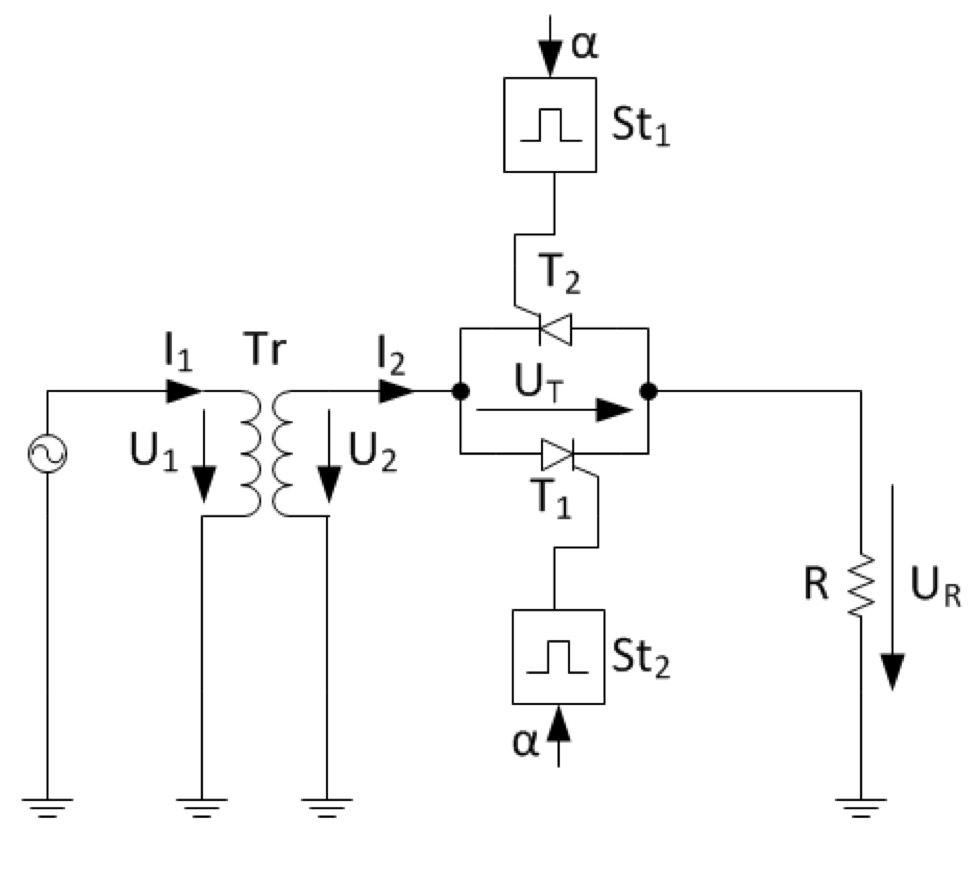
\includegraphics[width=0.85\linewidth]{images/Wechselstromsteller.png}
\end{center}

\begin{center}
    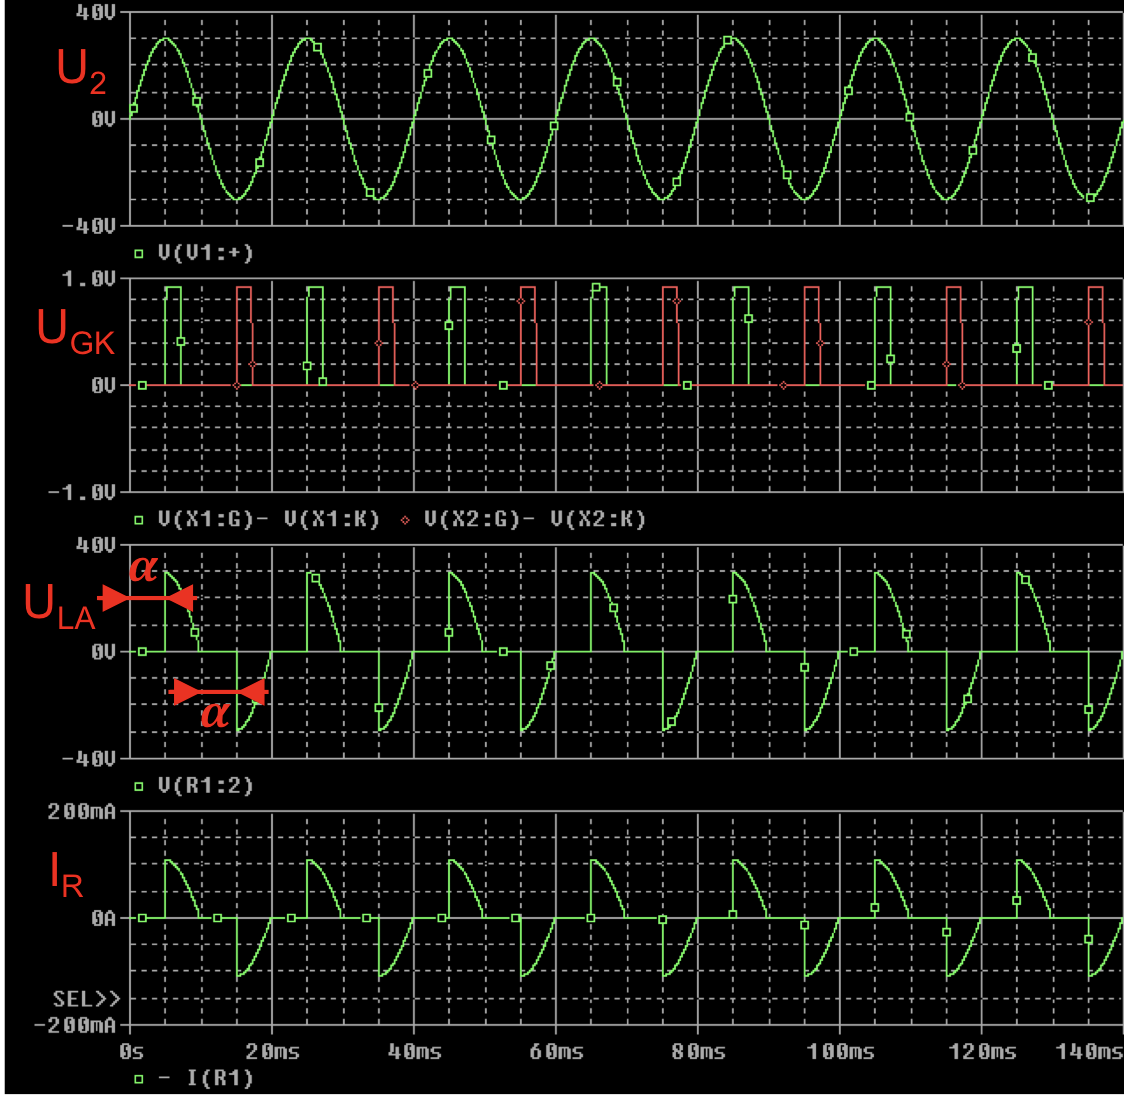
\includegraphics[width=0.85\linewidth]{images/Wechselstromsteller_Verlauf.png}
\end{center}
Eigenschaften:
\begin{itemize}
    \item Starke niederfrequente Harmonische.
    \item Abhängigkeit der Amplituden von $\alpha$.
    \item Ungerade und gerade Harmonische möglich.
\end{itemize}

\subsubsection{Rechteckwechselrichter}

Für symmetrische Rechteckspannung:
\[
\cbl{u(t) = \frac{4 U_{\mathrm{DC}}}{\pi}
\sum_{k=1,3,5,\dots}^{\infty} \frac{1}{k} \sin(k \omega t).}
\]

Eigenschaften:
\begin{itemize}
    \item Nur ungerade Harmonische.
    \item Amplituden $\sim 1/k$.
\end{itemize}

\subsubsection{PWM-Wechselrichter}

Eigenschaften:
\begin{itemize}
    \item Grundschwingung bei $f_1$.
    \item Seitenbänder um Vielfache der Schaltfrequenz $f_s$.
    \item Hochfrequente Harmonische dominieren.
\end{itemize}




\subsection{Effektivwert und Harmonische}

Der Gesamt-Effektivwert ergibt sich aus:
\[
\cbl{U_{\mathrm{RMS}}^2 = \sum_{n=1}^{\infty} U_{n,\mathrm{RMS}}^2.}
\]

Dabei:
\begin{itemize}
    \item $U_{1,\mathrm{RMS}}$: Grundschwingung
    \item $U_{n,\mathrm{RMS}}$: Harmonische Ordnung $n$
\end{itemize}

\subsection{Verzerrungsfaktor und THD}

\subsubsection{Total Harmonic Distortion (THD)}

Definition:
\[
\cbl{\mathrm{THD} =
\frac{\sqrt{ \sum_{n=2}^{\infty} U_{n,\mathrm{RMS}}^2 }}{U_{1,\mathrm{RMS}}}.}
\]

\paragraph{Leistungsfaktor bei nichtsinusförmigen Strömen}
\[
\lambda = \nu \cdot \cos\varphi_1 = \frac{U_{1,\mathrm{RMS}}}{U_{\mathrm{RMS}}} \cos\varphi_1
\]


Interpretation:
\begin{itemize}
    \item THD = 0: reiner Sinus
    \item THD gross: starke Verzerrung
\end{itemize}

\subsubsection{Verzerrungsfaktor}

\[
\cbl{\nu = \frac{U_{1,\mathrm{RMS}}}{U_{\mathrm{RMS}}}.}
\]

Beziehung:
\[
\cbl{\nu = \frac{1}{\sqrt{1 + \mathrm{THD}^2}}.}
\]

Dabei gilt:
\[
\nu = \frac{U_{1,\mathrm{RMS}}}{U_{\mathrm{RMS}}}
\]


\subsection{Wirkleistung und Harmonische}

Die Wirkleistung ergibt sich nur aus der Grundschwingung bei linearen Lasten:

\[
\cbl{P = U_{1,\mathrm{RMS}} \, I_{1,\mathrm{RMS}} \cos(\varphi_1).}
\]

Harmonische:
\begin{itemize}
    \item Erhöhen Effektivwert.
    \item Erzeugen Zusatzverluste.
    \item Tragen nicht zur Nutzleistung bei.
\end{itemize}

\crd{\textrightarrow\ Harmonische \textbf{verschlechtern Wirkungsgrad und Netzqualität}.}

\subsection{Filterwirkung der Last}

Bei R-L-Last:
\begin{itemize}
    \item Induktivität dämpft hohe Frequenzen.
    \item Strom ist sinusförmiger als Spannung.
\end{itemize}

Übertragungsfunktion:
\[
\cbl{|I_n| = \frac{|U_n|}{\sqrt{R^2 + (n \omega L)^2}}.}
\]

\paragraph{Stromharmonische bei R-L-Last}
Übertragungsfunktion der R--L-Last:
\[
\boxed{H(j\omega) = \frac{1}{R + j\omega L}}
\]
Stromamplitude der $n$-ten Harmonischen:
\[
I_n = \frac{U_n}{\sqrt{R^2 + (n\omega L)^2}}
\]


\subsection{Spektrale Bewertung von Umrichtern}

Typische Kenngrössen:
\begin{itemize}
    \item THD der Ausgangsspannung
    \item THD des Ausgangsstroms
    \item Oberwellenordnung mit maximaler Amplitude
    \item Anteil der Grundschwingung
\end{itemize}

\subsection{Typische Merksätze (Prüfungskern)}

\begin{itemize}
    \item \cbl{$U_{\mathrm{RMS}}^2 = \sum U_{n,\mathrm{RMS}}^2$}
    \item \cbl{$\mathrm{THD} = \dfrac{\sqrt{\sum_{n=2}^\infty U_n^2}}{U_1}$}
    \item Nur Grundschwingung liefert Wirkleistung.
    \item PWM verschiebt Harmonische in hohe Frequenzen.
\end{itemize}

\subsection{Typische Fehlerquellen}

\begin{itemize}
    \item Gesamt-$U_{\mathrm{RMS}}$ mit $U_{1,\mathrm{RMS}}$ verwechselt.
    \item THD mit Verzerrungsfaktor gleichgesetzt.
    \item Harmonische zur Wirkleistung addiert.
    \item Filterwirkung der Induktivität ignoriert.
\end{itemize}

\subsection{Minimal-Checkliste für Aufgaben}

\begin{enumerate}
    \item Signalform identifizieren (Rechteck, PWM, Anschnitt).
    \item Fourier-Koeffizienten bestimmen.
    \item Grundschwingung extrahieren.
    \item $U_{\mathrm{RMS}}$ aus Summenformel berechnen.
    \item THD berechnen.
    \item Einfluss der Lastinduktivität bewerten.
\end{enumerate}

        \section{PWM-Grundlagen und Modulation}
\subsection*{Definition der verwendeten Grössen}

\begin{itemize}
    \item $u_{\mathrm{ref}}(t)$: Referenzspannung (Sinus),
    \item $u_{\mathrm{tri}}(t)$: Trägerspannung (Dreieck),
    \item $\hat U_{\mathrm{ref}}$: Scheitelwert der Referenzspannung,
    \item $\hat U_{\mathrm{tri}}$: Scheitelwert der Trägerspannung,
    \item $m_a$: Amplitudenmodulationsindex,
    \item $f_1$: Grundfrequenz der Referenz,
    \item $f_s$: Träger- bzw. Schaltfrequenz,
    \item $U_{DC}$: Zwischenkreisspannung.
\end{itemize}

\subsection{Grundidee der Pulsweitenmodulation}

% --- bestehende Grafik: Sinus-Dreieck-Vergleich ---
\begin{center}
    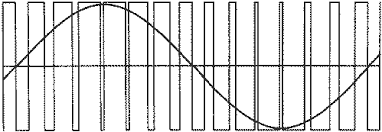
\includegraphics[width=0.85\linewidth]{images/sinuspwm.png}
\end{center}

Bei der Sinus-PWM wird:

\begin{itemize}
    \item Referenz: $u_{\mathrm{ref}}(t) = \hat U \sin(\omega t)$
    \item Träger: Dreieckspannung mit Frequenz $f_s$
\end{itemize}

Schaltregel:
\[
\text{Schalter EIN, wenn } u_{\mathrm{ref}}(t) > u_{\mathrm{tri}}(t)
\]

\subsection{Modulationsgrad}

\[
\cbl{m = \frac{\hat U_{\mathrm{ref}}}{\hat U_{\mathrm{tri}}}}
\]

Grundschwingungsamplitude:
\[
\cbl{\hat U_1 = m \cdot U_{DC}}
\]

Aussage:
\begin{itemize}
    \item $0 \le m \le 1$ linearer Modulationsbereich
    \item Amplitude proportional zu $m$
\end{itemize}

\subsection{Schaltfrequenz}

\[
\cbl{f_s \gg f_1}
\]

Eigenschaften:
\begin{itemize}
    \item Hohe $f_s$ $\Rightarrow$ gute Spektralqualität
    \item Hohe $f_s$ $\Rightarrow$ höhere Schaltverluste
\end{itemize}
\subsection{Grundschwingungsamplitude bei Sinus-PWM}

Für lineare Modulation ($m_a \le 1$) gilt:

\[
\boxed{\hat U_1 = m_a \frac{U_{DC}}{2}}
\]

Effektivwert:
\[
\boxed{U_{1,\mathrm{RMS}} = m_a \frac{U_{DC}}{2\sqrt{2}}}
\]

\subsection{Spektrum der PWM}

% --- bestehende Grafik: PWM-Spektrum ---
\begin{center}
    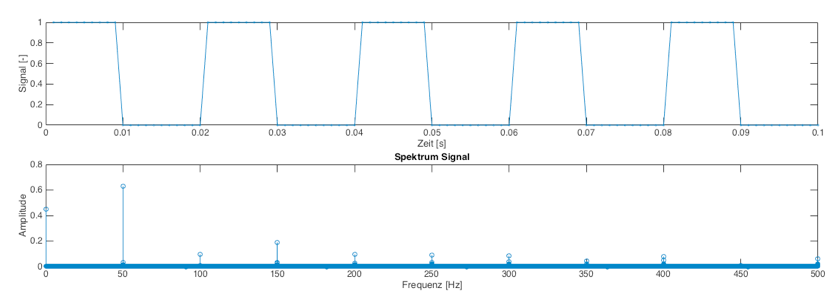
\includegraphics[width=0.85\linewidth]{images/specpwm.png}
\end{center}
Eigenschaften:
\begin{itemize}
    \item Grundschwingung bei $f_1$
    \item Seitenbänder um Vielfache von $f_s$
    \item Tiefpassfilter erzeugt nahezu Sinus
\end{itemize}

\crd{\textrightarrow\ PWM erlaubt getrennte Einstellung von Frequenz und Amplitude.}

        \section{Wechselrichter}

Ein Wechselrichter wandelt eine konstante Gleichspannung $U_{DC}$ in eine
\textbf{wechselnde Ausgangsspannung} mit vorgegebener Frequenz, Amplitude und Phase.
Er ist das zentrale Stellglied in \textbf{USV-Anlagen}, \textbf{Photovoltaiksystemen} und
\textbf{elektrischen Antrieben}.

Ziel des Wechselrichters ist:
\begin{itemize}
    \item Erzeugung einer sinusförmigen Grundschwingung,
    \item Steuerung von Amplitude und Frequenz,
    \item kontrollierter Leistungsfluss zwischen DC- und AC-Seite.
\end{itemize}

\subsection*{Definition der verwendeten Grössen}

\begin{itemize}
    \item $U_{DC}$: Zwischenkreisspannung (Gleichspannung),
    \item $u_2(t)$: momentane Ausgangsspannung,
    \item $i_2(t)$: momentaner Laststrom,
    \item $f_1$: Grundfrequenz der Ausgangsspannung,
    \item $\omega = 2\pi f_1$: Kreisfrequenz,
    \item $f_s$: Schaltfrequenz der PWM,
    \item $m_a$: Amplitudenmodulationsindex,
    \item $R$: Lastwiderstand,
    \item $L$: Lastinduktivität,
    \item $\varphi$: Phasenverschiebung zwischen Grundspannung und Grundstrom.
\end{itemize}

% ============================================================
\subsection{Einphasiger Wechselrichter}

\subsubsection{Grundschaltung: H-Brücke}

\begin{center}
    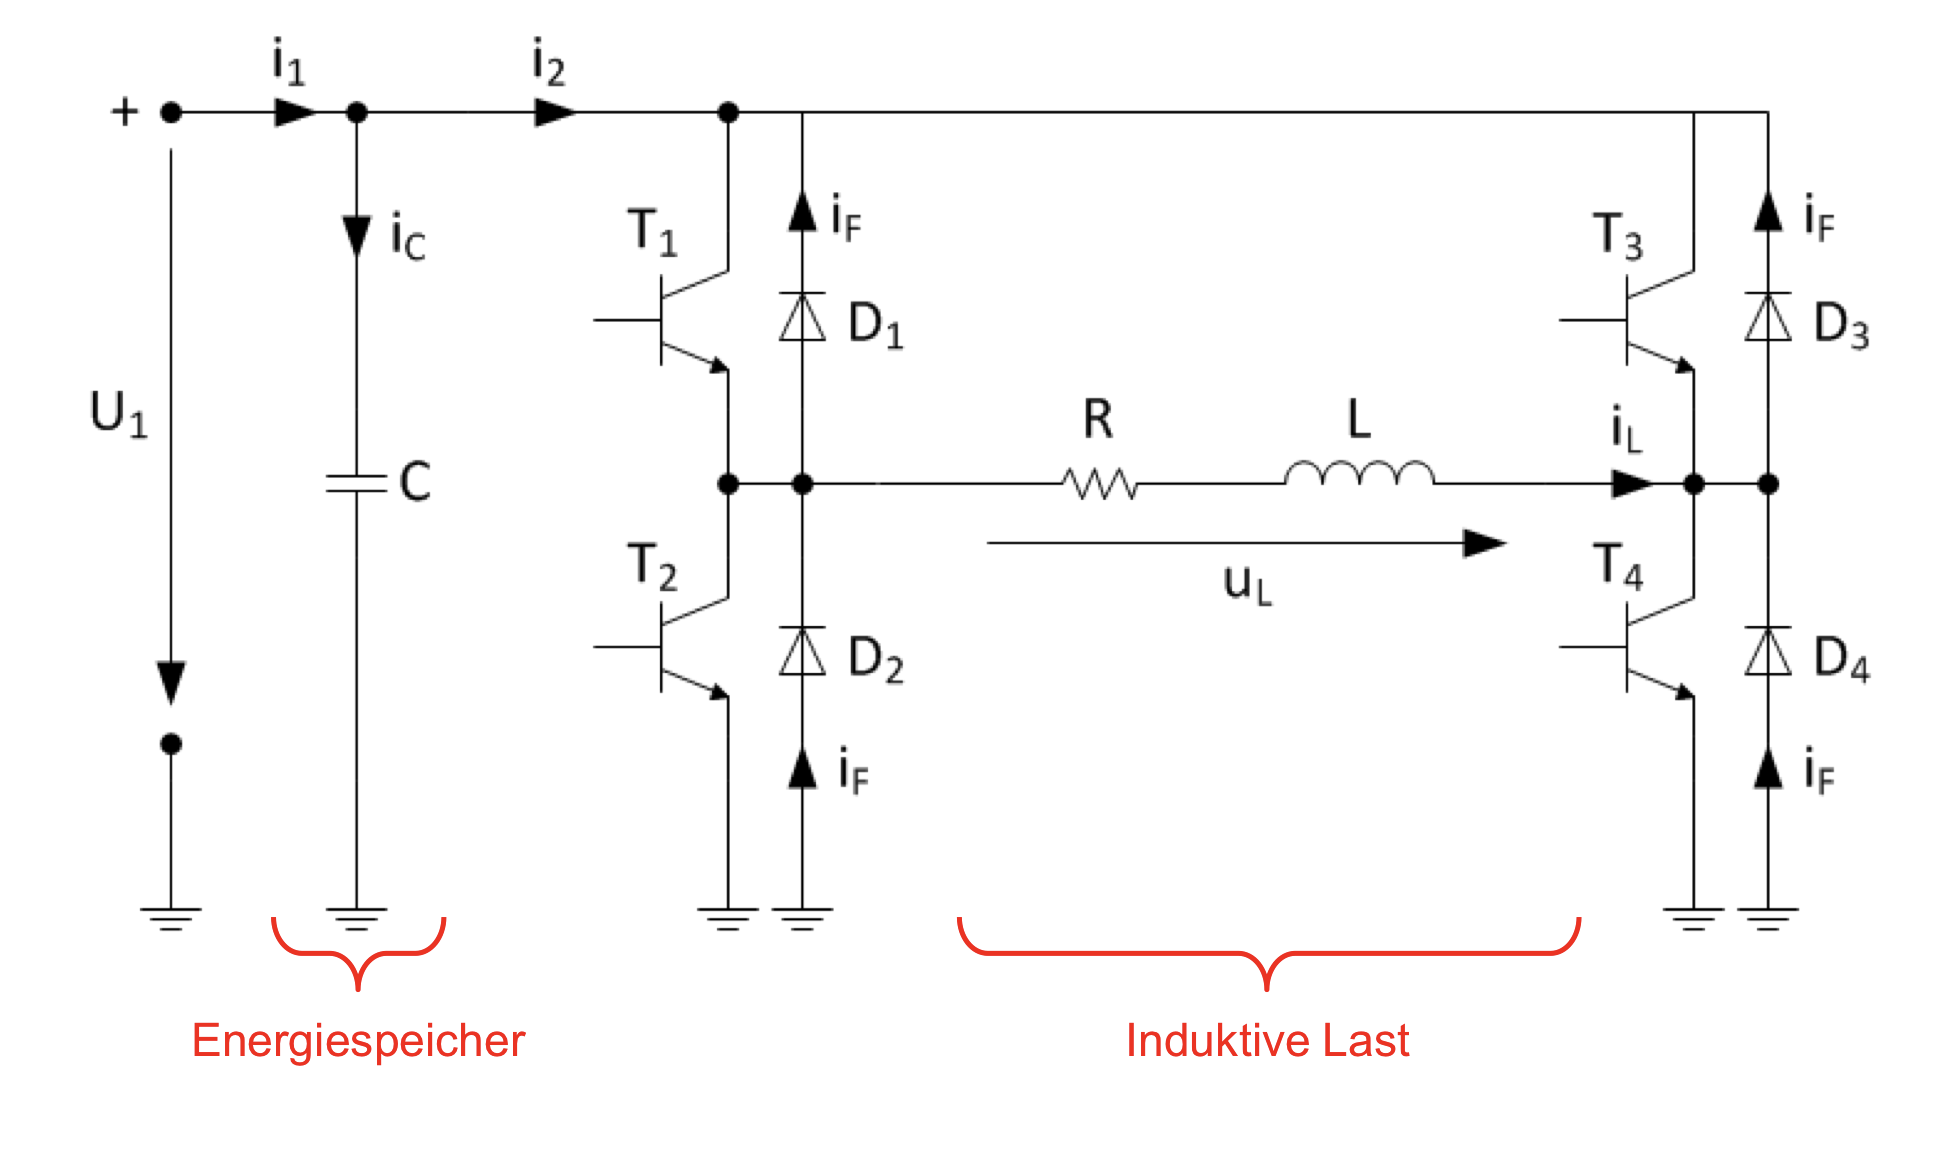
\includegraphics[width=0.85\linewidth]{images/1PWechselrichter.png}
\end{center}

Der einphasige Wechselrichter besteht aus einer H-Brücke mit vier steuerbaren Schaltern.
Durch geeignete Ansteuerung wird am Ausgang abwechselnd $+U_{DC}$ und $-U_{DC}$ erzeugt.
Die Last sieht dadurch eine periodische Wechselspannung.

Zulässige Ausgangsspannungen:
\[
\boxed{u_2(t) \in \{-U_{DC},\; 0,\; +U_{DC}\}}
\]

\subsubsection{Rechteckbetrieb}

Im Grundbetrieb wird mit 50\,\% Tastgrad geschaltet.

\begin{center}
    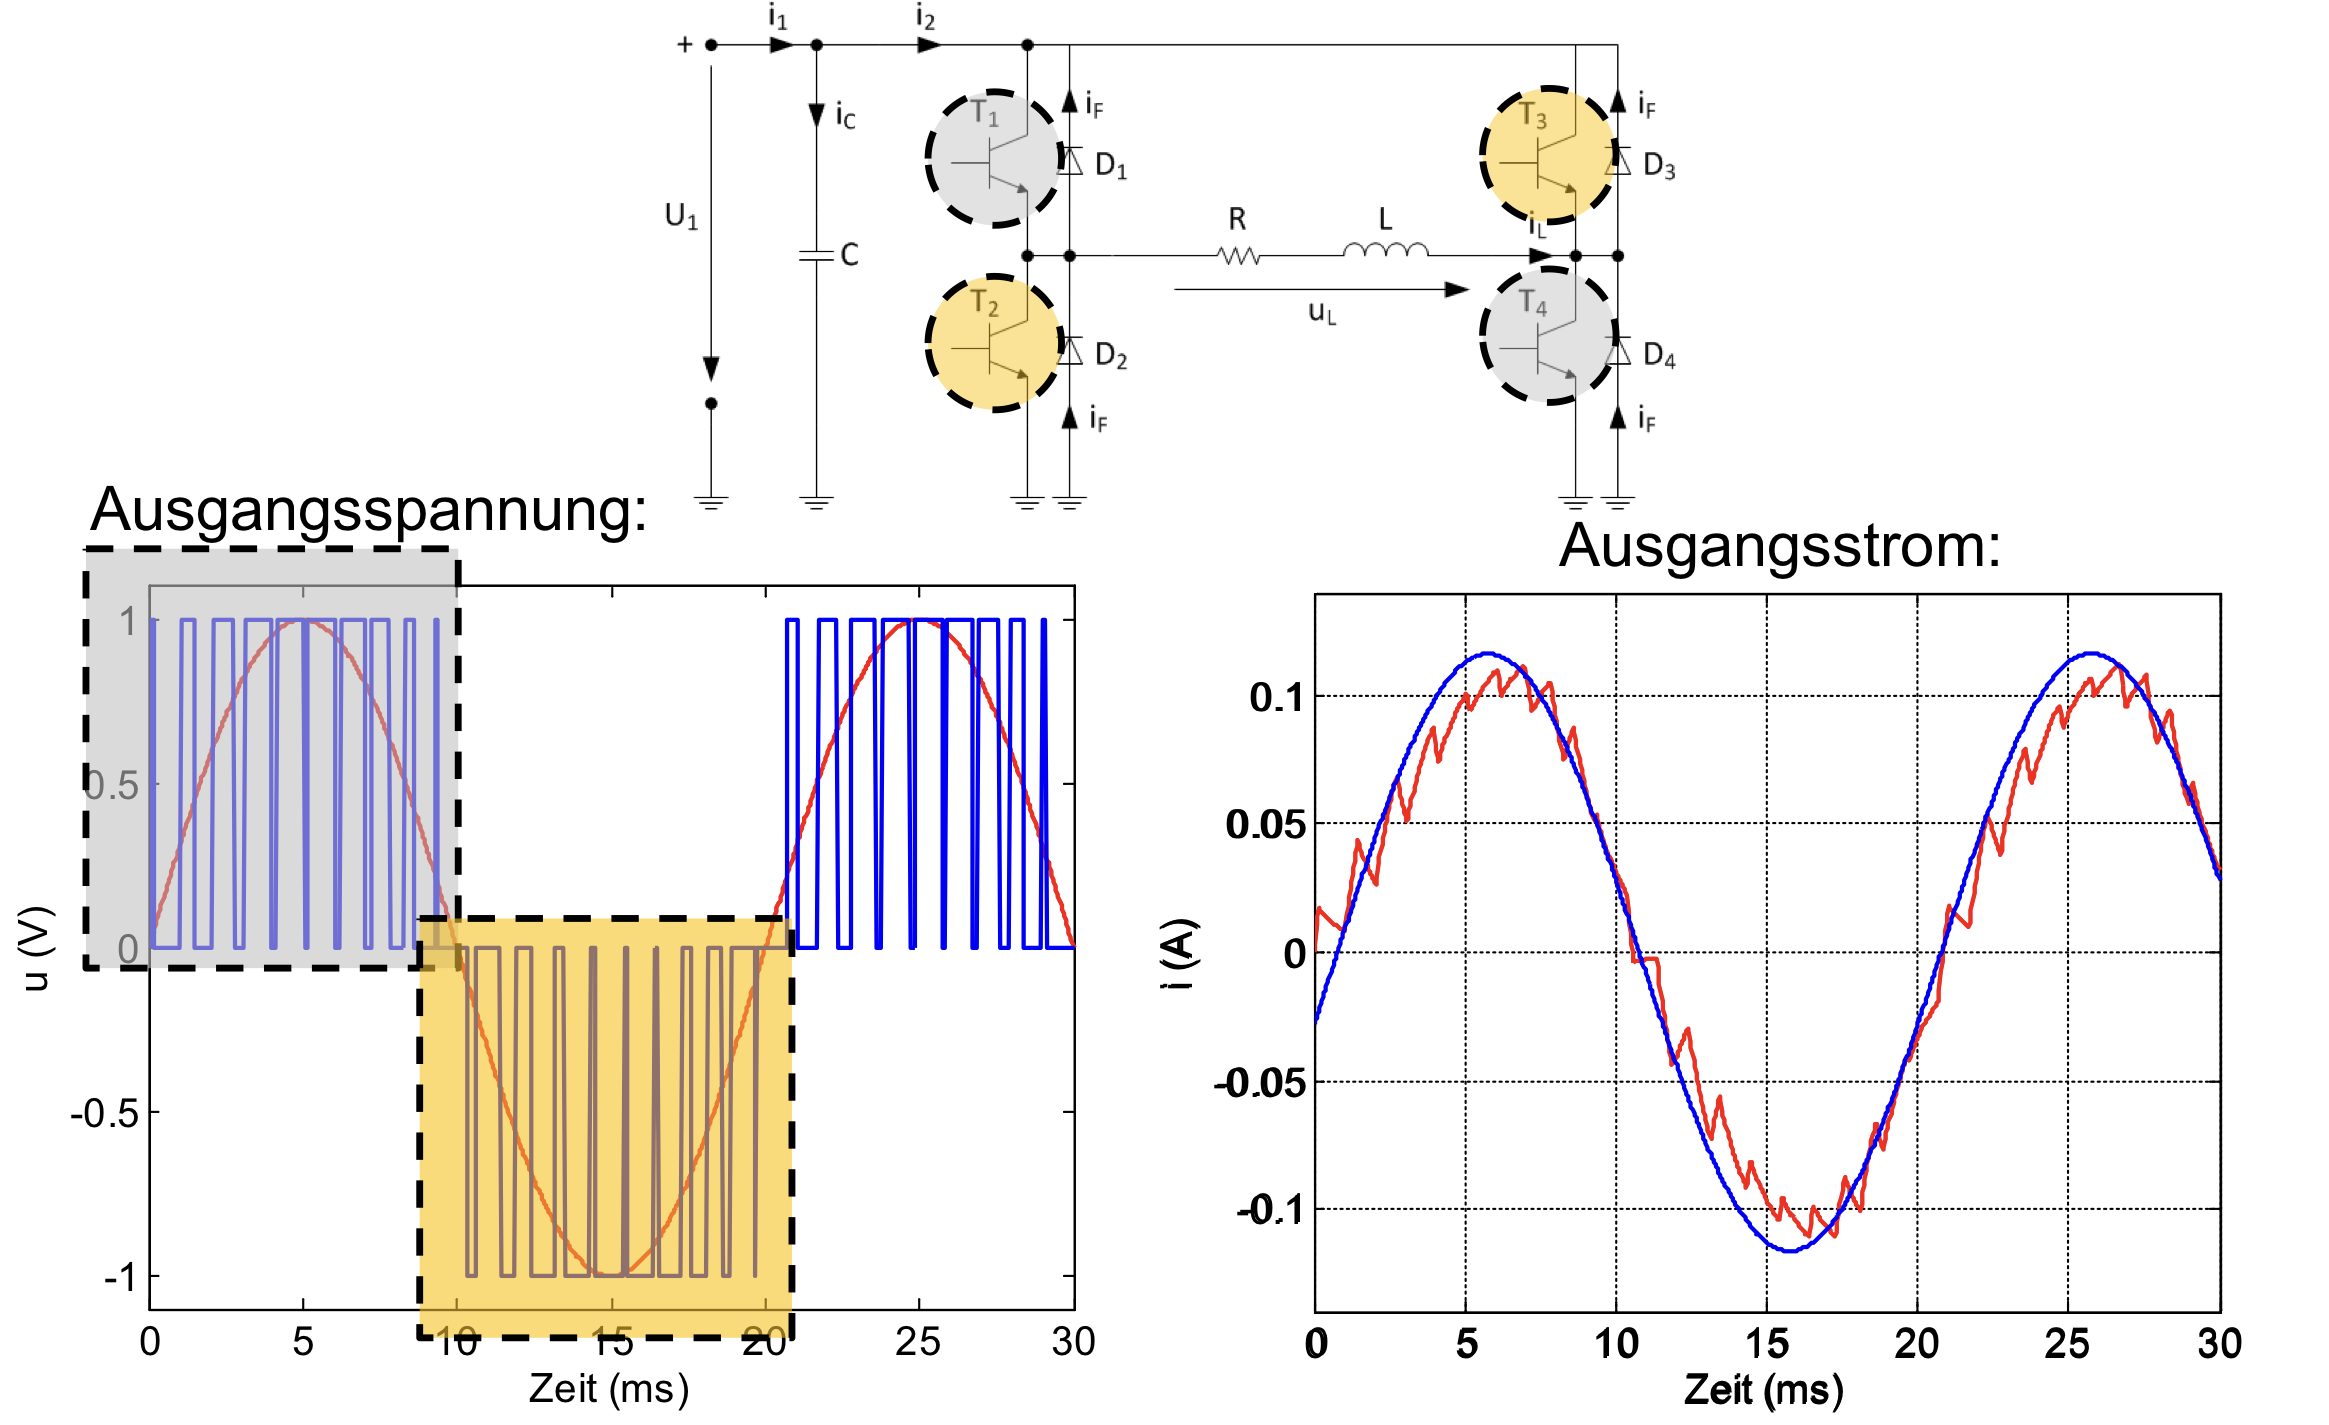
\includegraphics[width=0.85\linewidth]{images/1PWechselrichter_verlauf.png}
\end{center}

Ausgangsspannung:
\[
u_2(t) =
\begin{cases}
+U_{DC}, & 0 < \omega t < \pi \\
- U_{DC}, & \pi < \omega t < 2\pi
\end{cases}
\]

Grundfrequenz:
\[
\boxed{f_1 = \frac{1}{T}}
\]

Effektivwert der Rechteckspannung:
\[
\boxed{U_{\mathrm{RMS}} = U_{DC}}
\]

\paragraph{Erklärung}

Der Rechteckbetrieb ist einfach, liefert jedoch eine stark verzerrte Spannung.
Die Amplitude ist fest durch $U_{DC}$ vorgegeben und nicht steuerbar.
Dieser Betrieb ist nur für einfache Anwendungen geeignet.

\subsubsection{Fourier-Entwicklung}

Fourier-Reihe der Rechteckspannung:
\[
\boxed{
u_2(t) = \frac{4U_{DC}}{\pi}
\left(
\sin\omega t + \frac{1}{3}\sin 3\omega t + \frac{1}{5}\sin 5\omega t + \ldots
\right)
}
\]

Grundschwingungsamplitude:
\[
\boxed{\hat U_1 = \frac{4}{\pi} U_{DC}}
\]

Effektivwert der Grundschwingung:
\[
\boxed{U_{1,\mathrm{RMS}} = \frac{4}{\pi\sqrt{2}} U_{DC}}
\]

\subsubsection{Strom bei R--L-Last}

Lastgleichung:
\[
\boxed{u_2(t) = R i_2(t) + L \frac{di_2(t)}{dt}}
\]

Phasenverschiebung:
\[
\boxed{\tan\varphi = \frac{\omega L}{R}}
\]

Grundstrom:
\[
\boxed{i_{2,1}(t) = \hat I_1 \sin(\omega t - \varphi)}
\]

\paragraph{Erklärung}

Die Induktivität glättet den Strom und verschiebt ihn phasenmäßig nach hinten.
Der Strom enthält deutlich weniger Oberschwingungen als die Spannung.
Freilaufpfade sind zwingend erforderlich.

\subsubsection{PWM-Betrieb (Sinus-PWM)}

Grundschwingungsamplitude:
\[
\boxed{\hat U_1 = m_a \frac{U_{DC}}{2}}, 
\qquad 0 \le m_a \le 1
\]

Effektivwert:
\[
\boxed{U_{1,\mathrm{RMS}} = m_a \frac{U_{DC}}{2\sqrt{2}}}
\]

Grundstrom:
\[
\boxed{I_{1,\mathrm{RMS}} = \frac{U_{1,\mathrm{RMS}}}{\sqrt{R^2 + (\omega L)^2}}}
\]

\paragraph{Erklärung}

Durch PWM kann die Amplitude stufenlos über $m_a$ eingestellt werden.
Die Grundschwingung ist nahezu sinusförmig.
Harmonische liegen um Vielfache der Schaltfrequenz $f_s$.

\subsubsection{Leistungsfluss}

Momentanleistung:
\[
p(t) = u_2(t) i_2(t)
\]

Wirkleistung der Grundschwingung:
\[
\boxed{P = U_{1,\mathrm{RMS}} I_{1,\mathrm{RMS}} \cos\varphi}
\]

Blindleistung:
\[
\boxed{Q = U_{1,\mathrm{RMS}} I_{1,\mathrm{RMS}} \sin\varphi}
\]

\subsubsection{Spezialfälle}

\paragraph{Leerlauf}

\[
\boxed{i_2(t) \approx 0}, 
\qquad
\boxed{P \approx 0}
\]

\paragraph{Kurzschluss}

\[
\boxed{R \approx 0}
\]
\[
\boxed{\frac{di_2}{dt} \approx \frac{u_2(t)}{L}}
\]
\[
\boxed{\left.\frac{di_2}{dt}\right|_{\max} = \frac{U_{DC}}{L}}
\]

% ============================================================
\subsection{Dreiphasiger Wechselrichter}

\subsubsection{Grundschaltung}

\begin{center}
    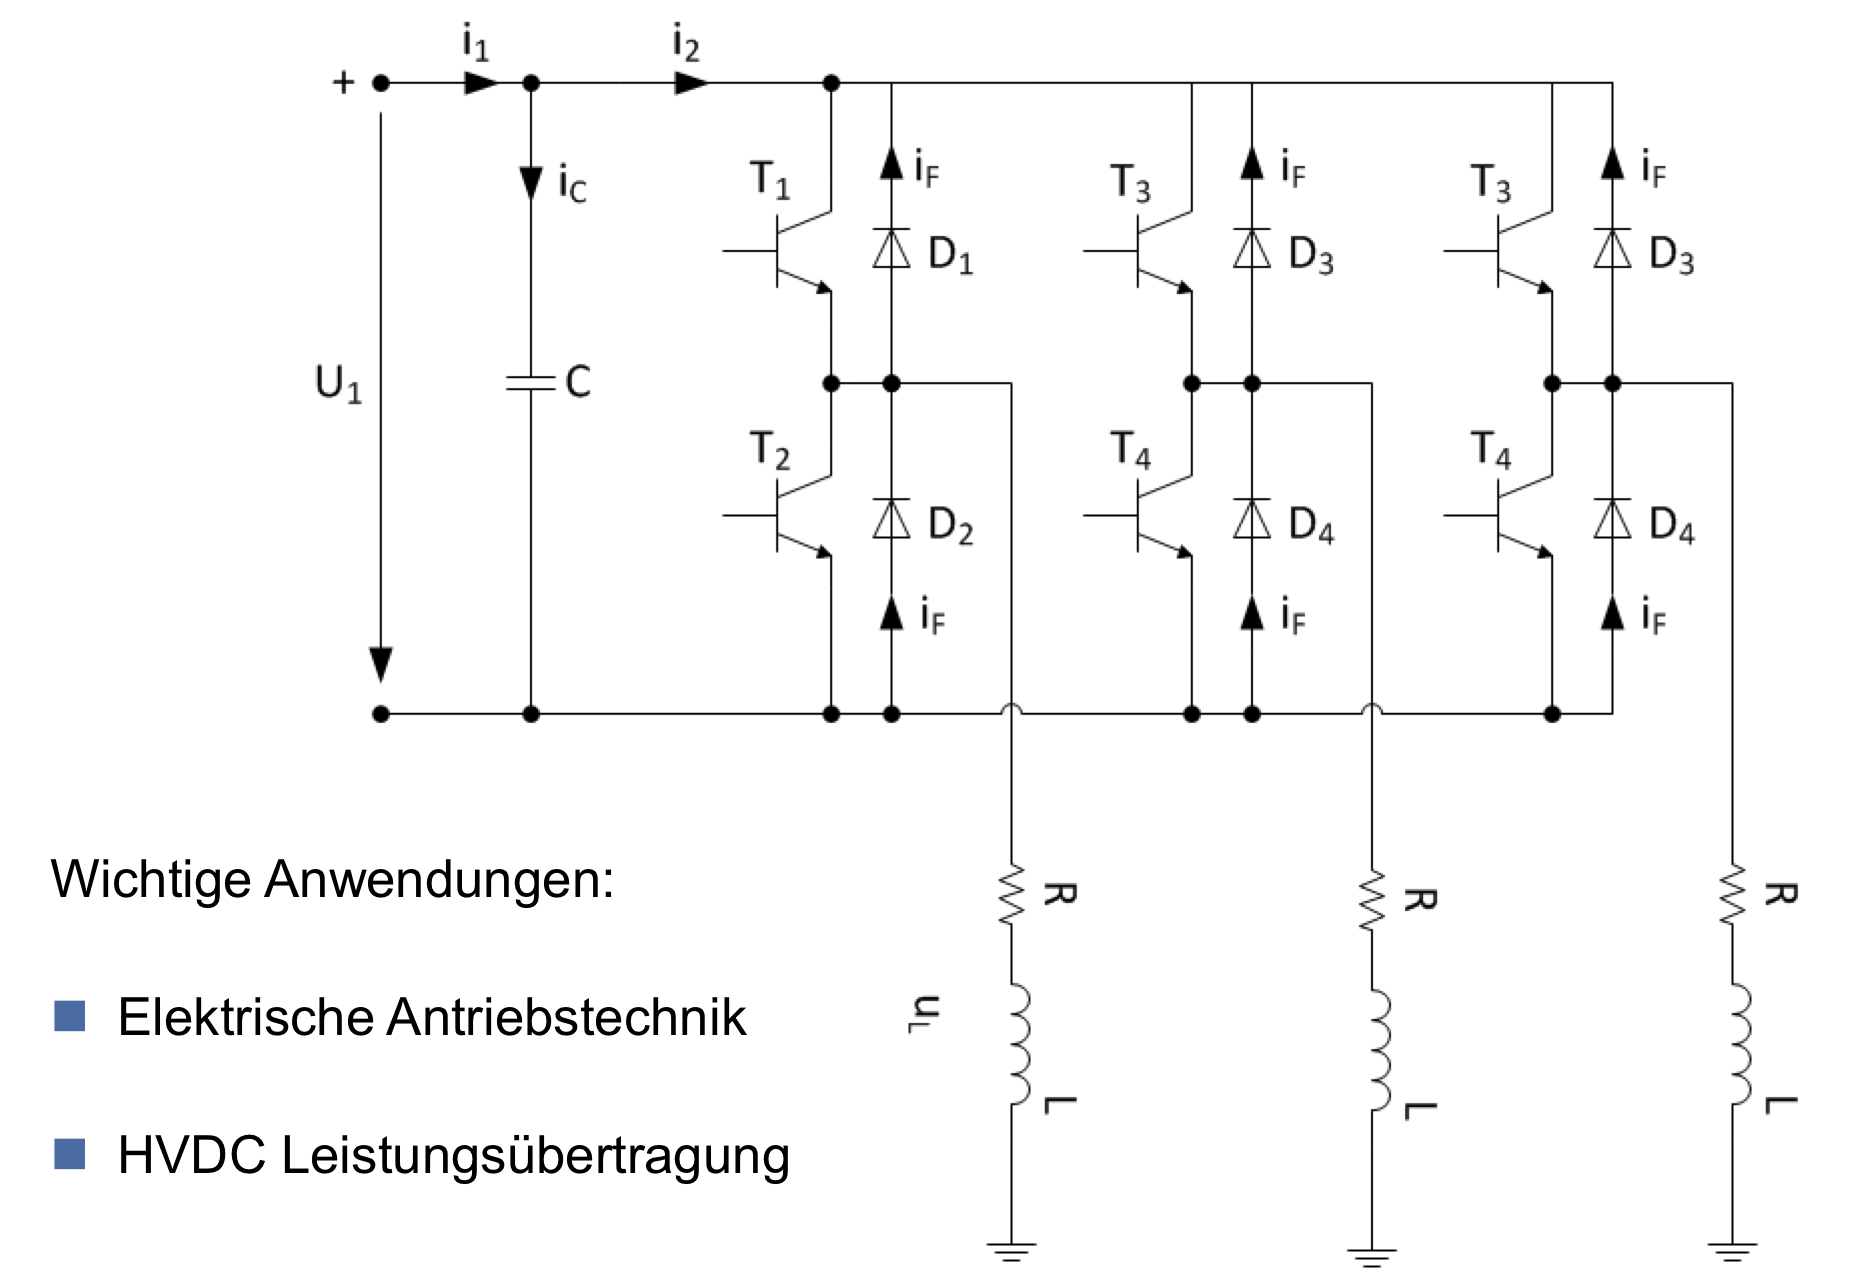
\includegraphics[width=0.85\linewidth]{images/3PWechselrichter.png}
\end{center}

Der dreiphasige Wechselrichter erzeugt drei um $120^\circ$ phasenverschobene Spannungen.
Er liefert bei symmetrischer Last einen nahezu konstanten Leistungsfluss.

Phasenspannungen:
\[
u_a(t),\; u_b(t),\; u_c(t)
\]

Leiterspannungen:
\[
\boxed{u_{ab} = u_a - u_b,\quad u_{bc} = u_b - u_c,\quad u_{ca} = u_c - u_a}
\]

\subsubsection{Grundschwingung}

Phasengrundspannung bei PWM:
\[
\boxed{U_{a,1} = \frac{m_a}{2} U_{DC}}
\]

Leitergrundspannung:
\[
\boxed{U_{LL,1} = \sqrt{3}\, U_{a,1}}
\]

\subsubsection{R--L-Last pro Phase}

Für jede Phase $k \in \{a,b,c\}$:
\[
\boxed{u_k(t) = R i_k(t) + L \frac{di_k}{dt}}
\]

Zeitkonstante:
\[
\boxed{\tau = \frac{L}{R}}
\]

Phasenströme:
\[
i_a(t) = \hat i \sin(\omega t - \varphi)
\]
\[
i_b(t) = \hat i \sin(\omega t - \varphi - \tfrac{2\pi}{3})
\]
\[
i_c(t) = \hat i \sin(\omega t - \varphi + \tfrac{2\pi}{3})
\]

\subsubsection{Leistung im symmetrischen Betrieb}

Mit Phasengrössen:
\[
\boxed{P = 3 U_{\mathrm{ph}} I_{\mathrm{ph}} \cos\varphi}
\]
\[
\boxed{Q = 3 U_{\mathrm{ph}} I_{\mathrm{ph}} \sin\varphi}
\]
\[
\boxed{S = 3 U_{\mathrm{ph}} I_{\mathrm{ph}}}
\]

Mit Leiterspannung:
\[
\boxed{P = \sqrt{3}\, U_{LL} I_L \cos\varphi}
\]

\paragraph{Erklärung}

Der dreiphasige Wechselrichter liefert bei symmetrischer Last einen konstanten Leistungsfluss.
Die Ströme sind sinusförmig und um $120^\circ$ verschoben.
Dieser Betrieb ist Standard in elektrischen Antrieben.

% ============================================================
\subsection{Vergleich Einphasig -- Dreiphasig}

\begin{center}
\begin{tabular}{l|c|c}
 & Einphasig & Dreiphasig \\ \hline
Phasen & 1 & 3 \\
Leistungsfluss & pulsierend & konstant \\
Oberschwingungen & hoch & geringer \\
Anwendungen & klein & Industrie \\
\end{tabular}
\end{center}

\subsection{Merksätze}

\begin{itemize}
    \item Wechselrichter: DC $\rightarrow$ AC mit steuerbarer Frequenz und Amplitude.
    \item Rechteckbetrieb: einfach, aber stark verzerrt.
    \item PWM: sinusförmige Grundschwingung, Amplitude über $m_a$ steuerbar.
    \item Induktive Last glättet den Strom.
    \item Dreiphasig: konstanter Leistungsfluss, Standard in Antrieben.
\end{itemize}

        \section{Direktumrichter (AC--AC-Umrichter ohne Zwischenkreis)}

Ein Direktumrichter wandelt eine dreiphasige Wechselspannung mit Frequenz $f_1$
\textbf{direkt} in eine Wechselspannung mit veränderlicher Frequenz $f_2$ und Amplitude,
\textbf{ohne Verwendung eines Gleichstrom-Zwischenkreises}.

Im Gegensatz zu Wechselrichtern erfolgt die Energiewandlung in \textbf{einem einzigen Schaltprozess}:
\[
\text{AC}_{f_1} \;\longrightarrow\; \text{AC}_{f_2}
\]

Typische Anwendungen:
\begin{itemize}
\item Niederdrehzahl-Grossantriebe,
\item Walzwerke,
\item Schiffantriebe,
\item Mühlen- und Ofenantriebe.
\end{itemize}

\subsection{Grundprinzip der direkten AC--AC-Wandlung}

% --- bestehende Grafik ---
\begin{center}
    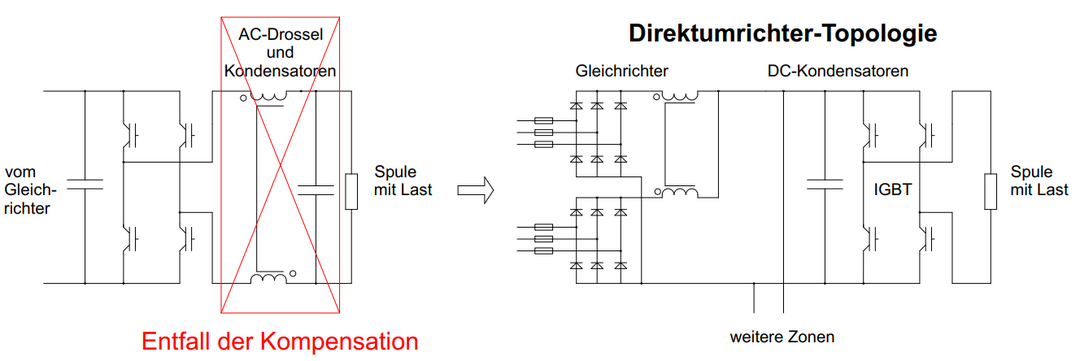
\includegraphics[width=0.85\linewidth]{images/direktumrichtergrund.png}
\end{center}

Der Direktumrichter verbindet jede Eingangsphase direkt mit jeder Ausgangsphase
über bidirektionale Schalter.

Mathematisch wird die Ausgangsspannung als zeitvariante Linearkombination
der Eingangsspannungen gebildet:

\[
\boxed{
\begin{bmatrix}
u_a(t)\\
u_b(t)\\
u_c(t)
\end{bmatrix}
=
\mathbf{M}(t)
\begin{bmatrix}
u_{R}(t)\\
u_{S}(t)\\
u_{T}(t)
\end{bmatrix}
}
\]

mit:

\begin{itemize}
    \item $u_{R},u_{S},u_{T}$: Eingangsphasenspannungen (Netz),
    \item $u_a,u_b,u_c$: Ausgangsphasenspannungen (Last),
    \item $\mathbf{M}(t)$: zeitabhängige Schaltmatrix mit Einträgen $m_{ij}(t) \in \{0,1\}$.
\end{itemize}

Jeder Matrixeintrag beschreibt:
\[
m_{ij}(t) =
\begin{cases}
1, & \text{Phase } j \text{ ist mit Ausgang } i \text{ verbunden} \\
0, & \text{sonst}
\end{cases}
\]

\crd{\textrightarrow\ Der Direktumrichter realisiert eine zeitvariable Abbildung zwischen Eingangs- und Ausgangsphasen.}

---

\subsection{Schaltungsstruktur (Matrixumrichter)}

% --- bestehende Grafik ---
\begin{center}
    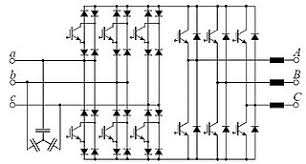
\includegraphics[width=0.85\linewidth]{images/direktumrichter_matrix.png}
\end{center}

Ein dreiphasiger Direktumrichter besitzt:

\[
\boxed{3 \times 3 = 9 \text{ bidirektionale Schalter}}
\]

Jeder Schalter muss:

\begin{itemize}
\item Strom in beide Richtungen leiten können,
\item Spannung in beide Richtungen sperren können,
\item kurzschluss- und unterbrechungsfrei schalten.
\end{itemize}

Typische Realisierung:
\[
\text{Bidirektionaler Schalter} = \text{2 antiparallele IGBTs mit Dioden}
\]

---

\subsection{Bildung der Ausgangsfrequenz}

Die Ausgangsspannung wird durch zeitliche Gewichtung der Eingangsphasen gebildet.

Idealisierte Darstellung für eine Ausgangsphase:

\[
\boxed{
u_a(t) = \alpha_R(t) u_R(t) + \alpha_S(t) u_S(t) + \alpha_T(t) u_T(t)
}
\]

mit:

\begin{itemize}
    \item $\alpha_R(t),\alpha_S(t),\alpha_T(t)$: zeitabhängige Schaltfunktionen,
    \item $\alpha_R+\alpha_S+\alpha_T = 1$ (keine Unterbrechung der Last).
\end{itemize}

Die Grundfrequenz der Ausgangsspannung ist:

\[
\boxed{f_2 = f_{\text{ref}}}
\]

wobei das Referenzsignal aus der Modulation erzeugt wird.

---

\subsection{Frequenzgrenze des Direktumrichters}

Die Ausgangsfrequenz ist durch die Kommutierung begrenzt:

\[
\boxed{f_2 < \frac{1}{2} f_1}
\]

Begründung:

\begin{itemize}
\item Jede Ausgangshalbwelle benötigt mehrere sichere Netzkommutierungen.
\item Die Netzspannung muss die Stromumlenkung erzwingen.
\item Bei zu hoher $f_2$ ist keine sichere Kommutierung mehr möglich.
\end{itemize}

Typischer Praxisbereich:
\[
f_2 \le 0.3 \, f_1
\]

---

\subsection{Leistungsfluss und Vierquadrantenbetrieb}

Momentanleistung:
\[
\boxed{p(t) = u_2(t)\, i_2(t)}
\]

Mittlere Leistung:
\[
\boxed{P = \frac{1}{T} \int_0^T u_2(t)\, i_2(t)\, dt}
\]

Da keine Diodenstrecken vorhanden sind, gilt:

\begin{itemize}
\item Strom kann Vorzeichen wechseln,
\item Spannung kann Vorzeichen wechseln,
\item Energie kann in beide Richtungen fliessen.
\end{itemize}

Damit ist möglich:

\[
\boxed{
(u,i) \in \{(+,+), (+,-), (-,+), (-,-)\}
}
\]

\crd{\textrightarrow\ Direktumrichter sind grundsätzlich vierquadrantenfähig.}

---

\subsection{Kommutierung als zentrales Problem}

% --- bestehende Grafik ---
\begin{center}
    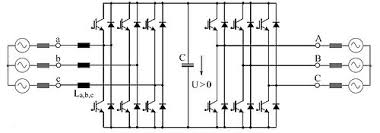
\includegraphics[width=0.85\linewidth]{images/direktumrichter_kommutierung.png}
\end{center}

Während der Kommutierung gilt zwingend:

\[
\boxed{
\begin{aligned}
&\text{Kein Kurzschluss zweier Netzphasen},\\
&\text{Kein Unterbrechen des Laststroms}.
\end{aligned}
}
\]

Formale Nebenbedingungen:

\[
\sum_{j \in \{R,S,T\}} m_{ij}(t) = 1 
\quad \forall i \in \{a,b,c\}
\]

und:

\[
\sum_{i \in \{a,b,c\}} m_{ij}(t) \le 1 
\quad \forall j \in \{R,S,T\}
\]

Bedeutung:

\begin{itemize}
\item Jede Lastphase ist immer mit genau einer Netzphase verbunden.
\item Keine zwei Lastphasen dürfen gleichzeitig dieselbe Netzphase kurzschliessen.
\end{itemize}

\crd{\textrightarrow\ Die Kommutierungslogik bestimmt die Komplexität des Direktumrichters.}

---

\subsection{Ausgangsströme bei R--L-Last}

Für jede Ausgangsphase gilt:

\[
\boxed{
u_k(t) = R i_k(t) + L \frac{di_k(t)}{dt},
\qquad k \in \{a,b,c\}
}
\]

Zeitkonstante:
\[
\boxed{\tau = \frac{L}{R}}
\]

Allgemeine Lösung bei konstantem $u_k$:

\[
\boxed{
i_k(t) = \frac{u_k}{R} + \left(i_k(t_0) - \frac{u_k}{R}\right) e^{-(t-t_0)/\tau}
}
\]

---

\subsection{Eigenschaften und Einordnung}

\begin{itemize}
    \item Sehr robuster Industrieumrichter.
    \item Hoher Wirkungsgrad (keine Zwischenkreisverluste).
    \item Begrenzter Frequenzbereich.
    \item Sehr komplexe Kommutierungssteuerung.
\end{itemize}

---

\subsection{Vergleich Direktumrichter -- Zwischenkreis-Wechselrichter}

\begin{center}
\begin{tabular}{l|c|c}
 & Direktumrichter & Wechselrichter \\ \hline
Zwischenkreis & nein & \cbl{ja} \\
Energiepuffer & keiner & \cbl{Kondensator} \\
AC--AC-Wandlung & direkt & \cbl{zweistufig} \\
Frequenzbereich & $f_2 < 0.5 f_1$ & \cbl{frei wählbar} \\
PWM notwendig & nein & \cbl{ja} \\
Kommutierung & netzgeführt & \cbl{selbstgeführt} \\
\end{tabular}
\end{center}

---

\subsection{Merksätze (Prüfungskern)}

\begin{itemize}
    \item Direktumrichter: direkte AC--AC-Wandlung ohne Zwischenkreis.
    \item Ausgangsspannung ist Linearkombination der Eingangsspannungen.
    \item Ausgangsfrequenz ist grundsätzlich begrenzt.
    \item Kommutierung ist das zentrale technische Problem.
    \item Vierquadrantenbetrieb ist ohne Zusatzschaltung möglich.
\end{itemize}

        \section{Mathematische Analyse -- Formelsammlung}

Diese Section sammelt die \textbf{wichtigsten mathematischen Werkzeuge}
für die Analyse in der Leistungselektronik:
\textbf{Ableitungen}, \textbf{Integrale}, \textbf{Trigonometrie},
\textbf{Exponentialfunktionen}, \textbf{Komplexrechnung},
\textbf{Laplace-Transformation} und \textbf{Differentialgleichungen (RLC)}.
Sie ist als \textbf{reine Nachschlage-Section} gedacht.

\smallskip

\textbf{Ziel:}
\begin{itemize}
    \item Schneller Zugriff auf Standardformeln
    \item Fehlerfreie Umformungen in Prüfungen
    \item Einheitliche Notation im ganzen Skript
\end{itemize}

% -------------------------------------------------
\subsection{Grundlegende Ableitungsregeln}

\subsubsection{Elementare Funktionen}

\[
\frac{d}{dx} c = 0
\qquad
\frac{d}{dx} x = 1
\qquad
\frac{d}{dx} x^n = n x^{n-1}
\]

\[
\frac{d}{dx} \e^{x} = \e^{x}
\qquad
\frac{d}{dx} \ln x = \frac{1}{x}
\]

\subsubsection{Lineare Regeln}

\[
\frac{d}{dx} [f(x) + g(x)] = f'(x) + g'(x)
\qquad
\frac{d}{dx} [c \, f(x)] = c \, f'(x)
\]

\subsubsection{Produktregel}

\[
\cbl{\frac{d}{dx} [f(x) g(x)] = f'(x) g(x) + f(x) g'(x)}
\]

\subsubsection{Quotientenregel}

\[
\cbl{\frac{d}{dx} \left[ \frac{f(x)}{g(x)} \right]
= \frac{f'(x) g(x) - f(x) g'(x)}{g(x)^2}}
\]

\subsubsection{Kettenregel}

\[
\cbl{\frac{d}{dx} f(g(x)) = f'(g(x)) \cdot g'(x)}
\]

% -------------------------------------------------
\subsection{Ableitungen trigonometrischer Funktionen}

\[
\cbl{\frac{d}{dx} \sin x = \cos x}
\qquad
\cbl{\frac{d}{dx} \cos x = - \sin x}
\]

\[
\frac{d}{dx} \tan x = \frac{1}{\cos^2 x}
\qquad
\frac{d}{dx} \cot x = - \frac{1}{\sin^2 x}
\]

\[
\frac{d}{dx} \arcsin x = \frac{1}{\sqrt{1-x^2}}
\qquad
\frac{d}{dx} \arccos x = -\frac{1}{\sqrt{1-x^2}}
\]

% -------------------------------------------------
\subsection{Grundlegende Integralregeln}

\subsubsection{Elementare Integrale}

\[
\int c \, dx = c x + C
\qquad
\int x^n \, dx = \frac{x^{n+1}}{n+1} + C \quad (n \neq -1)
\]

\[
\int \frac{1}{x} \, dx = \ln |x| + C
\qquad
\int \e^{x} \, dx = \e^{x} + C
\]

\subsubsection{Lineare Regeln}

\[
\int [f(x) + g(x)] dx = \int f(x) dx + \int g(x) dx
\qquad
\int c f(x) dx = c \int f(x) dx
\]

% -------------------------------------------------
\subsection{Integrale trigonometrischer Funktionen}

\[
\cbl{\int \sin x \, dx = - \cos x + C}
\qquad
\cbl{\int \cos x \, dx = \sin x + C}
\]

\[
\int \tan x \, dx = - \ln |\cos x| + C
\qquad
\int \cot x \, dx = \ln |\sin x| + C
\]

\[
\int \sin^2 x \, dx = \frac{x}{2} - \frac{\sin(2x)}{4} + C
\qquad
\int \cos^2 x \, dx = \frac{x}{2} + \frac{\sin(2x)}{4} + C
\]

\[
\int \sin(ax) \, dx = -\frac{1}{a}\cos(ax) + C
\qquad
\int \cos(ax) \, dx = \frac{1}{a}\sin(ax) + C
\]

% -------------------------------------------------
\subsection{Partielle Integration}

\[
\cbl{\int u \, dv = u v - \int v \, du}
\]

Beispiel:
\[
\int x \e^{x} dx = x \e^{x} - \int \e^{x} dx = (x-1) \e^{x} + C
\]

% -------------------------------------------------
\subsection{Substitution}

\[
\cbl{u = g(x), \qquad du = g'(x) dx}
\]

Beispiel:
\[
\int \sin(3x) dx
= -\frac{1}{3} \cos(3x) + C
\]

% -------------------------------------------------
\subsection{Trigonometrische Identitäten}

\subsubsection{Grundidentitäten}

\[
\cbl{\sin^2 x + \cos^2 x = 1}
\qquad
\cbl{1 + \tan^2 x = \frac{1}{\cos^2 x}}
\qquad
1 + \cot^2 x = \frac{1}{\sin^2 x}
\]

\subsubsection{Winkeladdition}

\[
\cbl{\sin(a \pm b) = \sin a \cos b \pm \cos a \sin b}
\]

\[
\cbl{\cos(a \pm b) = \cos a \cos b \mp \sin a \sin b}
\]

\subsubsection{Doppelwinkel}

\[
\cbl{\sin(2x) = 2 \sin x \cos x}
\qquad
\cbl{\cos(2x) = \cos^2 x - \sin^2 x = 1 - 2 \sin^2 x = 2 \cos^2 x - 1}
\]

\subsubsection{Halbwinkel}

\[
\cbl{\sin^2\left(\frac{x}{2}\right) = \frac{1-\cos x}{2}}
\qquad
\cbl{\cos^2\left(\frac{x}{2}\right) = \frac{1+\cos x}{2}}
\]

% -------------------------------------------------
\subsection{Produkt--Summen--Formeln}

\[
\cbl{\sin a \cos b = \frac{1}{2} [ \sin(a+b) + \sin(a-b) ]}
\]

\[
\cbl{\cos a \cos b = \frac{1}{2} [ \cos(a+b) + \cos(a-b) ]}
\]

\[
\cbl{\sin a \sin b = \frac{1}{2} [ \cos(a-b) - \cos(a+b) ]}
\]

\[
\cbl{\sin a + \sin b = 2 \sin\left(\frac{a+b}{2}\right) \cos\left(\frac{a-b}{2}\right)}
\]

\[
\cbl{\cos a + \cos b = 2 \cos\left(\frac{a+b}{2}\right) \cos\left(\frac{a-b}{2}\right)}
\]

\[
\cbl{\cos a - \cos b = -2 \sin\left(\frac{a+b}{2}\right) \sin\left(\frac{a-b}{2}\right)}
\]

% -------------------------------------------------
\subsection{Exponential- und Euler-Formeln}

\subsubsection{Euler-Formel}

\[
\cbl{\e^{\jimg x} = \cos x + \jimg \sin x}
\qquad
\cbl{\e^{-\jimg x} = \cos x - \jimg \sin x}
\]

\[
\cbl{\cos x = \frac{\e^{\jimg x} + \e^{-\jimg x}}{2}}
\qquad
\cbl{\sin x = \frac{\e^{\jimg x} - \e^{-\jimg x}}{2\jimg}}
\]

\subsubsection{Komplexe Sinusdarstellung}

\[
\cbl{\hat X \sin(\omega t + \varphi) = \Im\left\{ \hat X \e^{\jimg(\omega t + \varphi)} \right\}}
\]

\[
\cbl{\hat X \cos(\omega t + \varphi) = \Re\left\{ \hat X \e^{\jimg(\omega t + \varphi)} \right\}}
\]

% -------------------------------------------------
\subsection{Komplexrechnung}

\subsubsection{Grundformen}

\[
\cbl{z = x + \jimg y}
\qquad
\cbl{z = r \e^{\jimg \varphi}}
\]

\[
r = |z| = \sqrt{x^2 + y^2}
\qquad
\varphi = \arg(z)
\]

\subsubsection{Konjugation}

\[
\cbl{\overline{z} = x - \jimg y}
\qquad
\cbl{z \overline{z} = |z|^2}
\]

\subsubsection{Multiplikation und Division}

\[
\cbl{z_1 z_2 = r_1 r_2 \e^{\jimg (\varphi_1 + \varphi_2)}}
\qquad
\cbl{\frac{z_1}{z_2} = \frac{r_1}{r_2} \e^{\jimg (\varphi_1 - \varphi_2)}}
\]

\subsubsection{Real- und Imaginärteil}

\[
\cbl{\Re(z) = x}
\qquad
\cbl{\Im(z) = y}
\]

% -------------------------------------------------
\subsection{Komplexe Wechselstromrechnung}

\subsubsection{Ableiten im Zeitbereich}

\[
\cbl{\frac{d}{dt} \e^{\jimg \omega t} = \jimg \omega \e^{\jimg \omega t}}
\]

\subsubsection{Impedanzen}

\[
\cbl{Z_R = R}
\qquad
\cbl{Z_L = \jimg \omega L}
\qquad
\cbl{Z_C = \frac{1}{\jimg \omega C}}
\]

\subsubsection{Serien- und Parallelschaltung}

\[
\cbl{Z_{\mathrm{Serie}} = Z_1 + Z_2 + \dots}
\]

\[
\cbl{\frac{1}{Z_{\mathrm{Par}}} = \frac{1}{Z_1} + \frac{1}{Z_2} + \dots}
\]

% -------------------------------------------------
\subsection{Fourierreihen periodischer Funktionen}

Darstellung einer \textbf{periodischen} Funktion $f(t)$ mit Periodendauer $T > 0$ durch eine Linearkombination von Sinus- und Kosinusfunktionen,
deren Frequenzen ganzzahlige Vielfache der Kreisfrequenz (Winkelgeschwindigkeit) $\omega_f = \frac{2 \pi}{T} = 2 \pi v$ sind. 

\smallskip

\textbf{Hinweis:} In \cbl{blau} ist jeweils die komplexe Fourier-Theorie abgebildet.
$$ \FR[f(t)] = \frac{a_0}{2} + \sum\limits _{n=1}^\infty \big[ a_n \cdot \cos(n \, \omega_f \, t) + b_n \cdot \sin(n \, \omega_f \, t) \big] $$
$$ \cbl{\FR[f(t)] = \sum\limits _{k = -\infty}^\infty \: \big( c_k \cdot \e^{\jimg \, k \, \omega_f \, t} \big)} $$


\subsubsection{Orthagonalitätsbeziehungen Basisfunktionen}

\begin{tabular}{ll}
    $\int \limits_{0}^{T} \cos(m \, \omega_f \, t) \cdot \cos(n \, \omega_f \, t) \, \diff t = 
    \begin{cases}
        T,              & m = n = 0 \\
        \frac{T}{2},    & m = n > 0 \\
        0,              & m \neq n
    \end{cases}$ 
    & $(m, \; n \in \mathbb{N}_0)$ \\
    \\
    $\int \limits_{0}^{T} \sin(m \, \omega_f \, t) \cdot \sin(n \, \omega_f \, t) \, \diff t =      		
    \begin{cases}
        \frac{T}{2},    & m = n     \\
        0,              & m \neq n
    \end{cases} $ 
    & $(m, \; n \in \mathbb{N})$    \\
    \\
    $\int \limits_{0}^{T} \cos(m \, \omega_f \, t) \cdot \sin(n \, \omega_f \, t) \, \diff t = 0$ 	
    & $(m \in \mathbb{N}_0, \; n \in \mathbb{N})$ 
\end{tabular}


\subsubsection{Berechnung der Fourier-Koeffizienten}

\textbf{$\bm{\frac{a_0}{2}}$ entspricht dem Mittelwert (Gleichstromanteil) der Funktion $\bm{f(t)}$ auf dem \\
Intervall [0 ; T)}

\smallskip

\renewcommand{\arraystretch}{2.5}
\begin{tabular}{l c l}
    $a_n = \frac{2}{T} \cdot \int \limits_{0}^{T} f(t) \cdot \cos(n \, \omega_f \, t) \, \diff t$                           & $(n = 0, \, 1, \, 2, \, \ldots)$                                                                  \\
    $b_n = \frac{2}{T} \cdot \int \limits_{0}^{T} f(t) \cdot \sin(n \, \omega_f \, t) \, \diff t$                           & $(n = 1, \, 2, \, 3, \, \ldots)$                                                                  \\	
    $\cbl{c_n = \overline{c_{-n}} = \frac{1}{T} \int \limits_0^T f(t) \cdot \e^{- \jimg \, n \, \omega_f \, t} \, \diff t}$ & $\cbl{(n = 0, \, 1, \, 2, \, \ldots)}$    & \textrightarrow\ Für $n = 0: \, c_0 = \frac{a_0}{2}$
\end{tabular}
\renewcommand{\arraystretch}{1}

\smallskip

\crd{ \textrightarrow\ Trigo-Produkte in Integralen in SUMMEN umwandeln!!}


\paragraph{Umrechnung der Fourierkoeffizienten}

\renewcommand{\arraystretch}{1.4}
\begin{tabular}{ll}
    $c_n = \overline{c_{-n}} = \frac{a_n - \jimg \, b_n }{2}$   & ($n = 0, \, 1, \, 2, \, \ldots \text{ wobei } b_0 = 0$)   \\
    $a_n = 2 \, \RE(c_n) = c_n + c_{-n}$                        & ($n = 0, \, 1, \, 2, \, \ldots$)                          \\
    $b_n = -2 \, \IM(c_n) = \jimg (c_n - c_{-n})$               & ($n = 1, \, 2, \, 3, \, \ldots$) 
\end{tabular}
\renewcommand{\arraystretch}{1}

\columnbreak


\subsubsection{Sätze zur Berechnung der Koeffizienten}

\paragraph{Symmetrie von Funktionen}

\begin{minipage}{0.48\linewidth}
    \begin{tabular}{l | c | c}
                    & gerade    & ungerade  \\ 
        \hline
        gerade      & gerade    & ungerade  \\
        \hline
        ungerade    & ungerade  & gerade    \\
    \end{tabular}
\end{minipage}
\hfill
\begin{minipage}{0.43\linewidth}
    \begin{tabular}{ll}
        gerade:     &  $f(-t) = f(t)$ \\
        \\ 
        ungerade:   & $f(-t) = - f(t)$ 
    \end{tabular}
\end{minipage}

\smallskip

\begin{tabular}{lll}
    $f(t)$ gerade   & $b_n = 0$                 & $a_n = \frac{4}{T} \cdot \int \limits_{0}^{\frac{T}{2}} f(t) \cdot \cos(n \, \omega_f \, t) \, \diff t$   \\    \medskip
                    & \cbl{$\IM(c_k) = 0$}      & \cbl{$c_n = \frac{a_n}{2}$ (reell)}                                                                       \\
    $f(t)$ ungerade & $a_n = 0$                 & $b_n = \frac{4}{T} \cdot \int \limits_{0}^{\frac{T}{2}} f(t) \cdot \sin(n \, \omega_f \, t) \, \diff t$   \\	
                    & \cbl{$\RE(c_k) = 0$}      & \cbl{$c_n = \jimg \frac{b_n}{2}$ (imaginär)}
\end{tabular}
    

\paragraph{Linearität}

$f(x)$ mit Koeffizienten $a_n^{(f)} , \, b_n^{(f)}$ \qquad $g(x)$ mit Koeffizienten $a_n^{(g)} , \, b_n^{(g)}$ \\
\textrightarrow\ $h(t) = r \cdot f(t) + s \cdot g(t)$ mit festem $s, \, r \in \mathbb{R}$

$$ a_n^{(h)} = r \cdot a_n^{(f)} + s \cdot a_n^{(g)} \qquad \qquad b_n^{(h)} = r \cdot b_n^{(f)} + s \cdot b_n^{(g)} $$


\paragraph{Zeitstreckung / -stauchung / -spiegelung ("Ähnlichkeit")}

$g(t) = f(r \cdot t)$ mit $0 \neq r \in \mathbb{R}$ \qquad \cor{$\omega_g = \frac{2 \pi}{T_g}$ in Basisfunktionen!}

$$ a_n^{(g)} = a_n^{(f)} \qquad \qquad b_n^{(g)} = \sgn(r) \cdot b_n^{(f)} $$

\paragraph{Zeitverschiebung}
$g(t) = f(t + t_0)$

\smallskip

\renewcommand{\arraystretch}{1.7}
\begin{tabular}{ll}
    $ a_n^{(g)} = \cos(n \, \omega_f \, t_0) \cdot a_n^{(f)} + \sin(n \, \omega_f \, t_0) \cdot b_n^{(f)}$      & $n = 0$ \quad [mit $b_0 = 0, \, 1, \, 2, \, \ldots$]  \\ 
    $ b_n^{(g)} = -\sin(n \, \omega_f \, t_0) \cdot a_n^{(f)} + \cos(n \, \omega_f \, t_0) \cdot  b_n^{(f)}$    & $n = 1, \, 2, \, 3, \, \ldots$                        \\	
    $ \cbl{c_k^{(g)} = \e^{\jimg \, k \, \omega_f \, t_0} \cdot c_k^{(f)}}$                                     & $\cbl{k  =1, \, 2, \, 3, \, \ldots}$
\end{tabular}
\renewcommand{\arraystretch}{1}

\paragraph{Orthogonalitätsintegrale (Fourier-Kern)}

\[
\cbl{\int_0^T \cos(m \omega t)\cos(n \omega t)\,dt =
\begin{cases}
T, & m=n=0 \\
\frac{T}{2}, & m=n>0 \\
0, & m\neq n
\end{cases}}
\]

\[
\cbl{\int_0^T \sin(m \omega t)\sin(n \omega t)\,dt =
\begin{cases}
\frac{T}{2}, & m=n \\
0, & m\neq n
\end{cases}}
\]

\[
\cbl{\int_0^T \sin(m \omega t)\cos(n \omega t)\,dt = 0}
\]
\subsubsection{Beispiele: Fourier-Koeffizienten}

In allen Beispielen gilt:
\[
\omega_f=\frac{2\pi}{T}, 
\qquad
a_n=\frac{2}{T}\int_{-T/2}^{T/2} f(t)\cos(n\omega_f t)\,dt,
\qquad
b_n=\frac{2}{T}\int_{-T/2}^{T/2} f(t)\sin(n\omega_f t)\,dt.
\]

Hilfsintegrale (werden unten direkt verwendet):
\[
\int \sin(\alpha t)\sin(\beta t)\,dt
=\frac{1}{2}\int\left[\cos((\alpha-\beta)t)-\cos((\alpha+\beta)t)\right]dt
\]
\[
\int \cos(\alpha t)\cos(\beta t)\,dt
=\frac{1}{2}\int\left[\cos((\alpha-\beta)t)+\cos((\alpha+\beta)t)\right]dt
\]
\[
\int \sin(\alpha t)\cos(\beta t)\,dt
=\frac{1}{2}\int\left[\sin((\alpha+\beta)t)+\sin((\alpha-\beta)t)\right]dt
\]

% ============================================================
\paragraph{A) Ungerade Funktionen ($a_n = 0$)}

Definition:
\[
f(-t)=-f(t)
\quad\Rightarrow\quad
\boxed{a_n=0}
\quad\text{und}\quad
b_n=\frac{4}{T}\int_0^{T/2} f(t)\sin(n\omega_f t)\,dt.
\]

% -----------------------------
\subparagraph{U1 (einfach): $f(t)=\sin(\omega_f t)$}

Symmetrie: ungerade $\Rightarrow a_n=0$.

Berechnung von $b_n$:
\[
b_n=\frac{4}{T}\int_0^{T/2}\sin(\omega_f t)\sin(n\omega_f t)\,dt
\]

Orthogonalität:
\[
\int_0^{T/2}\sin(\omega_f t)\sin(n\omega_f t)\,dt=
\begin{cases}
\frac{T}{4}, & n=1\\
0, & n\neq 1
\end{cases}
\]

Damit:
\[
\boxed{b_1=\frac{4}{T}\cdot\frac{T}{4}=1},
\qquad
\boxed{b_{n\neq 1}=0},
\qquad
\boxed{a_n=0}.
\]

% -----------------------------
\subparagraph{U2 (mittel): Sägezahn $f(t)=\dfrac{2}{T}t$ auf $[-T/2,T/2]$}

Definition:
\[
f(t)=\frac{2}{T}t,\qquad t\in[-T/2,T/2],\quad \text{periodisch}
\]
Ungerade $\Rightarrow a_n=0$.

Berechnung:
\[
b_n=\frac{4}{T}\int_0^{T/2}\frac{2}{T}t\sin(n\omega_f t)\,dt
=\frac{8}{T^2}\int_0^{T/2} t\sin(n\omega_f t)\,dt
\]

Partielle Integration:
\[
\int t\sin(kt)\,dt=-\frac{t\cos(kt)}{k}+\frac{\sin(kt)}{k^2}
\]
mit $k=n\omega_f$.

Also:
\[
\int_0^{T/2} t\sin(n\omega_f t)\,dt=
\left[-\frac{t\cos(n\omega_f t)}{n\omega_f}+\frac{\sin(n\omega_f t)}{(n\omega_f)^2}\right]_0^{T/2}
\]

Einsetzen der Grenzen:
\[
\sin\!\left(n\omega_f \frac{T}{2}\right)=\sin(n\pi)=0,
\qquad
\cos\!\left(n\omega_f \frac{T}{2}\right)=\cos(n\pi)=(-1)^n
\]

Damit:
\[
\int_0^{T/2} t\sin(n\omega_f t)\,dt
=
-\frac{(T/2)(-1)^n}{n\omega_f}
\]

Also:
\[
b_n=\frac{8}{T^2}\left(-\frac{T}{2}\frac{(-1)^n}{n\omega_f}\right)
=-\frac{4}{T}\frac{(-1)^n}{n\omega_f}
\]

Mit $\omega_f=\frac{2\pi}{T}$ folgt:
\[
\boxed{
b_n=-\frac{4}{T}\frac{(-1)^n}{n}\cdot\frac{T}{2\pi}
=
-\frac{2}{\pi}\frac{(-1)^n}{n}
=
\frac{2}{\pi}\frac{(-1)^{n+1}}{n}
}
\]
\[
\boxed{a_n=0}
\]

% -----------------------------
\subparagraph{U3 (schwierig): stückweise linear ungerade (Dreiecksignal)}

Definition auf $[-T/2,T/2]$ (Amplitude $A$):
\[
f(t)=
\begin{cases}
\frac{2A}{T}t + A, & -\frac{T}{2}\le t < 0\\[4pt]
-\frac{2A}{T}t + A, & 0\le t \le \frac{T}{2}
\end{cases}
\]
Diese Funktion ist \textbf{ungerade?} Prüfen:
Für $t>0$ gilt $f(-t)=\frac{2A}{T}(-t)+A = -\frac{2A}{T}t + A = f(t)$.
Das wäre \textbf{gerade}, nicht ungerade.

Damit korrigiert ungerades Dreieck (Null in $t=0$):
\[
f(t)=
\begin{cases}
\frac{2A}{T}t, & 0\le t\le \frac{T}{2}\\[4pt]
\frac{2A}{T}t, & -\frac{T}{2}\le t<0
\end{cases}
\quad \text{(das ist linear und ungerade, entspricht Sägezahn)}
\]

Für ein \textbf{echtes ungerades Dreieck} (spitz bei $\pm T/4$) nimmt man z.B.:
\[
f(t)=
\begin{cases}
\frac{4A}{T}t, & 0\le t<\frac{T}{4}\\[4pt]
-\frac{4A}{T}t+2A, & \frac{T}{4}\le t\le \frac{T}{2}
\end{cases}
\quad \text{und ungerade fortsetzen}
\]

Dann:
\[
a_n=0,\qquad
b_n=\frac{4}{T}\left(
\int_0^{T/4}\frac{4A}{T}t\sin(n\omega_f t)\,dt
+
\int_{T/4}^{T/2}\left(-\frac{4A}{T}t+2A\right)\sin(n\omega_f t)\,dt
\right)
\]

Hinweis: Beide Integrale werden mit partieller Integration gelöst (wie in U2).
Das Ergebnis zeigt typischerweise ein $\sim 1/n^2$-Abklingen (typisch für Dreieck).

% ============================================================
\paragraph{B) Gerade Funktionen ($b_n = 0$)}

Definition:
\[
f(-t)=f(t)
\quad\Rightarrow\quad
\boxed{b_n=0}
\quad\text{und}\quad
a_n=\frac{4}{T}\int_0^{T/2} f(t)\cos(n\omega_f t)\,dt.
\]

% -----------------------------
\subparagraph{G1 (einfach): $f(t)=\cos(\omega_f t)$}

Gerade $\Rightarrow b_n=0$.

\[
a_n=\frac{4}{T}\int_0^{T/2}\cos(\omega_f t)\cos(n\omega_f t)\,dt
\]

Orthogonalität:
\[
\int_0^{T/2}\cos(\omega_f t)\cos(n\omega_f t)\,dt=
\begin{cases}
\frac{T}{4}, & n=1\\
0, & n\neq 1
\end{cases}
\]

Damit:
\[
\boxed{a_1=1},\qquad \boxed{a_{n\neq 1}=0},\qquad \boxed{b_n=0}.
\]

% -----------------------------
\subparagraph{G2 (mittel): $f(t)=\sin^2(\omega_f t)$}

Gerade, weil $\sin^2$ gerade ist.

Umformung:
\[
\sin^2(\omega_f t)=\frac{1}{2}\big(1-\cos(2\omega_f t)\big)
\]

Vergleich mit Fourier-Reihe:
\[
f(t)=\frac{a_0}{2}+a_2\cos(2\omega_f t)
\]

Damit:
\[
\boxed{\frac{a_0}{2}=\frac{1}{2}\Rightarrow a_0=1},
\qquad
\boxed{a_2=-\frac{1}{2}},
\qquad
\boxed{a_{n\neq 0,2}=0},
\qquad
\boxed{b_n=0}.
\]

% -----------------------------
\subparagraph{G3 (schwierig): gerade Rechteckfunktion mit Rechenweg}

Definition (Amplitude $A$):
\[
f(t)=
\begin{cases}
A, & |t|<\frac{T}{4}\\
-A, & \frac{T}{4}<|t|<\frac{T}{2}
\end{cases}
\quad \text{periodisch}
\]

Gerade $\Rightarrow b_n=0$.

\[
a_n=\frac{4}{T}\int_0^{T/2} f(t)\cos(n\omega_f t)\,dt
=\frac{4}{T}\left(
\int_0^{T/4} A\cos(n\omega_f t)\,dt
+\int_{T/4}^{T/2} (-A)\cos(n\omega_f t)\,dt
\right)
\]

\[
a_n=\frac{4A}{T}\left(
\int_0^{T/4}\cos(n\omega_f t)\,dt
-\int_{T/4}^{T/2}\cos(n\omega_f t)\,dt
\right)
\]

Mit
\[
\int \cos(n\omega_f t)\,dt=\frac{1}{n\omega_f}\sin(n\omega_f t)
\]

folgt:
\[
a_n=\frac{4A}{T}\cdot\frac{1}{n\omega_f}
\left[
\sin\!\left(n\omega_f\frac{T}{4}\right)-\sin(0)
-\Big(\sin(n\omega_f\frac{T}{2})-\sin(n\omega_f\frac{T}{4})\Big)
\right]
\]

\[
a_n=\frac{4A}{T}\cdot\frac{1}{n\omega_f}
\left[
2\sin\!\left(n\omega_f\frac{T}{4}\right)-\sin\!\left(n\omega_f\frac{T}{2}\right)
\right]
\]

Einsetzen:
\[
n\omega_f\frac{T}{4}=n\frac{2\pi}{T}\frac{T}{4}=\frac{n\pi}{2},
\qquad
n\omega_f\frac{T}{2}=n\pi
\Rightarrow \sin(n\pi)=0
\]

Damit:
\[
\boxed{
a_n=\frac{4A}{T}\cdot\frac{1}{n\omega_f}\cdot 2\sin\!\left(\frac{n\pi}{2}\right)
}
\]

Mit $\omega_f=\frac{2\pi}{T}$:
\[
\boxed{
a_n=\frac{4A}{n\pi}\sin\!\left(\frac{n\pi}{2}\right),
\qquad
b_n=0
}
\]

\paragraph{C) Weder gerade noch ungerade ($a_n$ und $b_n$)}

Wenn keine Symmetrie vorliegt, müssen \textbf{beide} Koeffizientenfamilien berechnet werden:

\[
a_n=\frac{2}{T}\int_{-T/2}^{T/2} f(t)\cos(n\omega_f t)\,dt,
\qquad
b_n=\frac{2}{T}\int_{-T/2}^{T/2} f(t)\sin(n\omega_f t)\,dt.
\]

Es gibt \textbf{keine Vereinfachung} durch Symmetrie.  
Jeder Koeffizient muss explizit integriert werden.

% -------------------------------------------------
\subparagraph{N1 (einfach): $f(t)=\sin(\omega_f t)+\cos(\omega_f t)$}

Zerlegung in Basisfunktionen:
\[
f(t)=\sin(\omega_f t)+\cos(\omega_f t)
\]

Vergleich mit Fourier-Ansatz:
\[
f(t)=a_1\cos(\omega_f t)+b_1\sin(\omega_f t)
\]

Direkt ablesbar:
\[
\boxed{a_1=1},\qquad \boxed{b_1=1},
\qquad
\boxed{a_{n\neq 1}=0},\qquad \boxed{b_{n\neq 1}=0}.
\]

Interpretation:
\begin{itemize}
    \item Beide Koeffizienten ungleich null.
    \item Keine Symmetrie vorhanden.
    \item Reine Grundschwingung mit Phasenverschiebung.
\end{itemize}

% -------------------------------------------------
\subparagraph{N2 (mittel): Phasenverschobener Sinus $f(t)=A\sin(\omega_f t+\varphi)$}

Ausgangsfunktion:
\[
f(t)=A\sin(\omega_f t+\varphi)
\]

Trigonometrische Zerlegung:
\[
\sin(\alpha+\beta)=\sin\alpha\cos\beta+\cos\alpha\sin\beta
\]

Damit:
\[
f(t)=A\sin(\omega_f t)\cos\varphi + A\cos(\omega_f t)\sin\varphi
\]

Vergleich mit Fourier-Reihe:
\[
f(t)=a_1\cos(\omega_f t)+b_1\sin(\omega_f t)
\]

Ablesen der Koeffizienten:
\[
\boxed{a_1=A\sin\varphi},\qquad
\boxed{b_1=A\cos\varphi}
\]
\[
\boxed{a_{n\neq 1}=0},\qquad \boxed{b_{n\neq 1}=0}.
\]

Interpretation:
\begin{itemize}
    \item Phase $\varphi$ verteilt Energie auf $a_1$ und $b_1$.
    \item Amplitude:
    \[
    \sqrt{a_1^2+b_1^2}=A
    \]
    \item Phasenlage:
    \[
    \tan\varphi=\frac{a_1}{b_1}
    \]
\end{itemize}

% -------------------------------------------------
\subparagraph{N3 (schwierig): Halbwellen-gleichgerichteter Sinus – vollständige Rechnung}

Definition mit $\theta=\omega_f t$, Periode $2\pi$:
\[
f(\theta)=
\begin{cases}
\sin\theta, & 0<\theta<\pi\\
0, & \pi<\theta<2\pi
\end{cases}
\]

Hier gilt:
\[
f(-\theta)\neq f(\theta),
\qquad
f(-\theta)\neq -f(\theta)
\]
also \textbf{keine Symmetrie}.

Allgemeine Koeffizienten (Periode $2\pi$):
\[
a_n=\frac{1}{\pi}\int_0^{2\pi} f(\theta)\cos(n\theta)\,d\theta,
\qquad
b_n=\frac{1}{\pi}\int_0^{2\pi} f(\theta)\sin(n\theta)\,d\theta.
\]

Da $f(\theta)=0$ für $\pi<\theta<2\pi$:
\[
a_n=\frac{1}{\pi}\int_0^{\pi} \sin\theta\cos(n\theta)\,d\theta,
\qquad
b_n=\frac{1}{\pi}\int_0^{\pi} \sin\theta\sin(n\theta)\,d\theta.
\]

% -----------------------------
\paragraph{Berechnung von $a_n$}

Produkt-zu-Summe:
\[
\sin\theta\cos(n\theta)=\frac{1}{2}
\Big[\sin((n+1)\theta)+\sin((1-n)\theta)\Big]
\]

Damit:
\[
a_n=\frac{1}{2\pi}\int_0^{\pi}
\Big[\sin((n+1)\theta)+\sin((1-n)\theta)\Big]\,d\theta
\]

Integration:
\[
\int \sin(k\theta)\,d\theta=-\frac{1}{k}\cos(k\theta)
\]

\[
a_n=\frac{1}{2\pi}
\left[
-\frac{\cos((n+1)\theta)}{n+1}
-\frac{\cos((1-n)\theta)}{1-n}
\right]_0^{\pi}
\]

Auswertung der Kosinus-Terme:
\[
\cos((n+1)\pi)=(-1)^{n+1},\qquad
\cos((1-n)\pi)=(-1)^{1-n}
\]

Nach Einsetzen und Vereinfachung erhält man:
\[
\boxed{
a_n=
\begin{cases}
0, & n \text{ ungerade} \\[6pt]
\dfrac{2}{\pi}\,\dfrac{1}{1-n^2}, & n \text{ gerade}
\end{cases}
}
\]

Insbesondere:
\[
\boxed{a_0=\frac{2}{\pi}} \quad \text{(DC-Anteil)}
\]

% -----------------------------
\paragraph{Berechnung von $b_n$}

Produkt-zu-Summe:
\[
\sin\theta\sin(n\theta)=\frac{1}{2}
\Big[\cos((n-1)\theta)-\cos((n+1)\theta)\Big]
\]

Damit:
\[
b_n=\frac{1}{2\pi}\int_0^{\pi}
\Big[\cos((n-1)\theta)-\cos((n+1)\theta)\Big]\,d\theta
\]

Integration:
\[
\int \cos(k\theta)\,d\theta=\frac{1}{k}\sin(k\theta)
\]

\[
b_n=\frac{1}{2\pi}
\left[
\frac{\sin((n-1)\theta)}{n-1}
-\frac{\sin((n+1)\theta)}{n+1}
\right]_0^{\pi}
\]

Da:
\[
\sin(k\pi)=0 \quad \forall k\in\mathbb{Z}
\]

folgt:
\[
\boxed{
b_n=
\begin{cases}
\dfrac{1}{2}, & n=1 \\[6pt]
0, & n\neq 1
\end{cases}
}
\]

% -----------------------------
\paragraph{Endergebnis für den halbwellen-gleichgerichteten Sinus}

Fourier-Reihe:
\[
f(\theta)=\frac{a_0}{2}
+\sum_{n=1}^\infty a_n\cos(n\theta)
+\sum_{n=1}^\infty b_n\sin(n\theta)
\]

mit:
\[
\boxed{a_0=\frac{2}{\pi}}
\]
\[
\boxed{
a_n=
\begin{cases}
\dfrac{2}{\pi}\,\dfrac{1}{1-n^2}, & n \text{ gerade}\\[6pt]
0, & n \text{ ungerade}
\end{cases}
}
\]
\[
\boxed{
b_1=\frac{1}{2},\qquad
b_{n\neq 1}=0
}
\]

Interpretation:
\begin{itemize}
    \item DC-Anteil vorhanden ($a_0\neq 0$).
    \item Sowohl Kosinus- als auch Sinusanteile treten auf.
    \item Typischer Prüfungsfall für „weder gerade noch ungerade“.
\end{itemize}


% ============================================================
\paragraph{Zusammenfassung}

\begin{itemize}
    \item Ungerade $\Rightarrow a_n=0$, nur $b_n$.
    \item Gerade $\Rightarrow b_n=0$, nur $a_n$.
    \item Weder noch $\Rightarrow$ beide vorhanden.
    \item Symmetrie spart die Hälfte der Integrale und eliminiert ganze Koeffizientenfamilien.
\end{itemize}

\paragraph{Merksätze (Final)}

\begin{itemize}
    \item Jede Funktion lässt sich in gerade und ungerade Anteile zerlegen.
    \item Symmetrie spart bis zu 50\% der Integrale.
    \item Zeitverschiebung erzeugt gleichzeitig $a_n$ und $b_n$.
    \item DC-Offset beeinflusst nur $a_0$.
    \item Rechteck, PWM, Gleichrichtung sind immer \textbf{weder gerade noch ungerade}.
\end{itemize}


% -------------------------------------------------
\subsection{Grenzwerte und Reihen}

\[
\cbl{\lim_{x \to 0} \frac{\sin x}{x} = 1}
\qquad
\cbl{\lim_{x \to 0} \frac{1 - \cos x}{x^2} = \frac{1}{2}}
\]

\[
\cbl{\e^{x} = \sum_{n=0}^{\infty} \frac{x^n}{n!}}
\qquad
\cbl{\sin x = \sum_{n=0}^{\infty} (-1)^n \frac{x^{2n+1}}{(2n+1)!}}
\qquad
\cbl{\cos x = \sum_{n=0}^{\infty} (-1)^n \frac{x^{2n}}{(2n)!}}
\]

% -------------------------------------------------
\subsection{Bestimmte Integrale über Perioden}

\[
\cbl{\int_0^T \sin(n \omega t)\,dt = 0}
\qquad
\cbl{\int_0^T \cos(n \omega t)\,dt = 0}
\]

\[
\cbl{\int_0^T \sin^2(n \omega t)\,dt = \frac{T}{2}}
\qquad
\cbl{\int_0^T \cos^2(n \omega t)\,dt = \frac{T}{2}}
\]

% =================================================
\subsection{Laplace-Transformation}

\subsubsection{Definition}

Für eine zeitkontinuierliche Funktion $f(t)$ (typisch $t\ge 0$):
\[
\cbl{\mathcal{L}\{f(t)\} = F(s) = \int_{0}^{\infty} f(t)\, \e^{-st}\,dt}
\qquad
s = \sigma + \jimg \omega
\]

\subsubsection{Wichtige Grundtransformierte}

\[
\mathcal{L}\{1\} = \frac{1}{s}
\qquad
\mathcal{L}\{t\} = \frac{1}{s^2}
\qquad
\mathcal{L}\{t^n\} = \frac{n!}{s^{n+1}}
\]

\[
\cbl{\mathcal{L}\{\e^{at}\} = \frac{1}{s-a}}
\]

\[
\cbl{\mathcal{L}\{\sin(\omega t)\} = \frac{\omega}{s^2+\omega^2}}
\qquad
\cbl{\mathcal{L}\{\cos(\omega t)\} = \frac{s}{s^2+\omega^2}}
\]

\[
\mathcal{L}\{\sinh(\omega t)\} = \frac{\omega}{s^2-\omega^2}
\qquad
\mathcal{L}\{\cosh(\omega t)\} = \frac{s}{s^2-\omega^2}
\]

\subsubsection{Linearität}

\[
\cbl{\mathcal{L}\{a f(t) + b g(t)\} = aF(s) + bG(s)}
\]

\subsubsection{Ableitungssatz}

\[
\cbl{\mathcal{L}\left\{\frac{df}{dt}\right\} = sF(s) - f(0)}
\]

\[
\cbl{\mathcal{L}\left\{\frac{d^2f}{dt^2}\right\} = s^2F(s) - s f(0) - f'(0)}
\]

\crd{\textrightarrow\ Anfangswerte gehen als Terme in den Zähler. Häufige Prüfungsfalle.}

\subsubsection{Integralsatz}

\[
\cbl{\mathcal{L}\left\{\int_0^t f(\tau)\,d\tau\right\} = \frac{1}{s} F(s)}
\]

\subsubsection{Zeitverschiebung (Heaviside)}

\[
\cbl{\mathcal{L}\{f(t-t_0)u(t-t_0)\} = \e^{-s t_0} F(s)}
\]

\subsubsection{Frequenzverschiebung}

\[
\cbl{\mathcal{L}\{\e^{at} f(t)\} = F(s-a)}
\]

\subsubsection{Faltung}

\[
\cbl{(f*g)(t) = \int_0^t f(\tau)g(t-\tau)\,d\tau}
\qquad
\cbl{\mathcal{L}\{f*g\} = F(s)G(s)}
\]

\subsubsection{Initial- und Finalwertsatz}

\[
\cbl{f(0^+) = \lim_{s\to\infty} sF(s)}
\qquad
\cbl{f(\infty) = \lim_{s\to 0} sF(s)}
\]

\crd{\textrightarrow\ Finalwertsatz nur gültig, wenn alle Pole von $sF(s)$ in der linken Halbebene liegen.}

\subsubsection{Inverse Laplace (Standardstrategien)}

\begin{itemize}
    \item Partialbruchzerlegung
    \item Tabellenrücktransformation
    \item Verschiebungssätze (Zeit, Frequenz)
    \item Quadratische Ergänzung für $s^2+\omega^2$
\end{itemize}

% =================================================
\subsection{Übertragungsfunktionen und Systemdarstellung}

Für lineare zeitinvariante Systeme (LTI):
\[
\cbl{H(s) = \frac{Y(s)}{X(s)}}
\]

\subsubsection{Pol-Nullstellen-Darstellung}

\[
\cbl{H(s)=K \frac{(s-z_1)(s-z_2)\dots}{(s-p_1)(s-p_2)\dots}}
\]

\subsubsection{Zeitkonstante und Eckfrequenz}

Erste Ordnung:
\[
\cbl{H(s)=\frac{1}{1+s\tau}}
\qquad
\cbl{\omega_c = \frac{1}{\tau}}
\qquad
\cbl{f_c = \frac{1}{2\pi\tau}}
\]

% =================================================
\subsection{Differentialgleichungen 1. Ordnung (R--L / R--C)}

\subsubsection{Standardform}

\[
\cbl{\tau \frac{dy}{dt} + y = K \, u(t)}
\]

Homogene Lösung:
\[
\cbl{y_h(t) = C \e^{-t/\tau}}
\]

Partikuläre Lösung (Konstantanregung $u(t)=U$):
\[
\cbl{y_p(t)=K U}
\]

Gesamtlösung:
\[
\cbl{y(t) = K U + \big(y(0)-K U\big)\e^{-t/\tau}}
\]

\subsubsection{R--L-Kreis}

\[
\cbl{L\frac{di}{dt} + Ri = u(t)}
\qquad
\cbl{\tau = \frac{L}{R}}
\]

Sprung $u(t)=U$:
\[
\cbl{i(t) = \frac{U}{R}\left(1-\e^{-t/\tau}\right) + i(0)\e^{-t/\tau}}
\]

\subsubsection{R--C-Kreis}

\[
\cbl{RC\frac{du_C}{dt} + u_C = u(t)}
\qquad
\cbl{\tau = RC}
\]

Sprung $u(t)=U$:
\[
\cbl{u_C(t) = U\left(1-\e^{-t/\tau}\right) + u_C(0)\e^{-t/\tau}}
\]

\crd{\textrightarrow\ Bei Induktivitäten ist $i(t)$ stetig, bei Kapazitäten ist $u_C(t)$ stetig.}

% =================================================
\subsection{Differentialgleichungen 2. Ordnung (RLC-Systeme)}

\subsubsection{Standardform}

\[
\cbl{\frac{d^2y}{dt^2} + 2\zeta\omega_0 \frac{dy}{dt} + \omega_0^2 y = K \omega_0^2 u(t)}
\]

\[
\cbl{\omega_0 = \sqrt{\frac{1}{LC}}}
\qquad
\cbl{\zeta = \frac{R}{2}\sqrt{\frac{C}{L}}}
\]

\subsubsection{Dämpfungsfälle}

\begin{itemize}
    \item \textbf{Unterdämpft:} $0<\zeta<1$ (schwingend)
    \item \textbf{Kritisch gedämpft:} $\zeta=1$
    \item \textbf{Überdämpft:} $\zeta>1$
\end{itemize}

Unterdämpfte Eigenfrequenz:
\[
\cbl{\omega_d = \omega_0\sqrt{1-\zeta^2}}
\]

\subsubsection{Freie Schwingung (homogene Lösung)}

Unterdämpft:
\[
\cbl{y_h(t)=\e^{-\zeta\omega_0 t}\left(C_1\cos(\omega_d t)+C_2\sin(\omega_d t)\right)}
\]

Überdämpft:
\[
\cbl{y_h(t)=C_1\e^{s_1 t}+C_2\e^{s_2 t}}
\qquad
s_{1,2}=-\omega_0\left(\zeta\pm\sqrt{\zeta^2-1}\right)
\]

Kritisch:
\[
\cbl{y_h(t)=(C_1 + C_2 t)\e^{-\omega_0 t}}
\]

\subsubsection{Serien-RLC (Stromdynamik)}

KVL:
\[
\cbl{u(t)=Ri(t)+L\frac{di}{dt}+\frac{1}{C}\int i(t)\,dt}
\]

Differenziert:
\[
\cbl{\frac{d^2 i}{dt^2} + \frac{R}{L}\frac{di}{dt} + \frac{1}{LC}i = \frac{1}{L}\frac{du}{dt}}
\]

\subsubsection{Parallele-RLC (Spannungsdynamik)}

KCL:
\[
i(t)=\frac{u(t)}{R}+C\frac{du}{dt}+\frac{1}{L}\int u(t)\,dt
\]

Differenziert:
\[
\cbl{\frac{d^2 u}{dt^2} + \frac{1}{RC}\frac{du}{dt} + \frac{1}{LC}u = \frac{1}{C}\frac{di}{dt}}
\]

\subsubsection{Laplace-Lösung von DGLs}

Vorgehen:
\begin{enumerate}
    \item DGL aufstellen (KVL/KCL)
    \item Laplace anwenden (Ableitungssätze)
    \item Nach $Y(s)$ auflösen
    \item Partialbrüche
    \item Rücktransformation
\end{enumerate}

\subsubsection{Standardübertragungsfunktionen}

\paragraph{Tiefpass 1. Ordnung}
\[
\cbl{H(s)=\frac{1}{1+s\tau}}
\]

\paragraph{Bandpass / Resonanz 2. Ordnung (Normalform)}
\[
\cbl{H(s)=\frac{\omega_0^2}{s^2+2\zeta\omega_0 s+\omega_0^2}}
\]

% -------------------------------------------------
\subsection{Konzeptionelles Vorgehen: lineare Differentialgleichungen}

In praktisch allen Aufgaben der Leistungselektronik folgt die Lösung derselben Struktur:
\[
u(x) = u_{\mathrm{hom}}(x) + u_{\mathrm{part}}(x),
\qquad
L[u] = g(x)
\Rightarrow
\begin{cases}
L[u_{\mathrm{hom}}] = 0, \\
L[u_{\mathrm{part}}] = g(x).
\end{cases}
\]

Dabei gilt:
\begin{itemize}
    \item $u_{\mathrm{hom}}$: Eigenverhalten des Systems (ohne Quelle),
    \item $u_{\mathrm{part}}$: Antwort auf die Anregung $g(x)$,
    \item Rand- und Anfangsbedingungen bestimmen die physikalisch zulässige Lösung.
\end{itemize}

Diese Zerlegung ist der \textbf{Standardalgorithmus} für alle linearen DGL in Umrichter-, R--L-, R--C- und Maschinenproblemen.

% -------------------------------------------------

\subsubsection{1. Typ der Differentialgleichung identifizieren}

Gegeben ist typischerweise eine lineare DGL mit konstanten Koeffizienten:
\[
a_n u^{(n)} + \dots + a_1 u' + a_0 u = g(x).
\]

Klassifikation:
\begin{itemize}
    \item \textbf{Homogen:} $g(x) = 0$ (freies Einschwingen, Ausschwingen).
    \item \textbf{Inhomogen:} $g(x) \neq 0$ (Quelle vorhanden).
    \item Ordnung = höchste Ableitung $n$.
\end{itemize}

In der Leistungselektronik dominieren:
\begin{itemize}
    \item 1. Ordnung: R--L, R--C,
    \item 2. Ordnung: L--C, gedämpfte Schwingkreise, Maschinenmodelle.
\end{itemize}

% -------------------------------------------------

\subsubsection{2. Homogene Lösung $u_{\mathrm{hom}}$}

Für konstante Koeffizienten wird angesetzt:
\[
u(x) = e^{\lambda x}.
\]

Einsetzen liefert die charakteristische Gleichung:
\[
a_n \lambda^n + \dots + a_1 \lambda + a_0 = 0.
\]

Standardfälle:

\paragraph{1. Ordnung}
\[
u' + a u = 0 
\quad \Rightarrow \quad 
u_{\mathrm{hom}} = C e^{-a x}.
\]

\paragraph{2. Ordnung, zwei reelle Nullstellen $\lambda_1,\lambda_2$}
\[
u_{\mathrm{hom}} = C_1 e^{\lambda_1 x} + C_2 e^{\lambda_2 x}.
\]

\paragraph{2. Ordnung, doppelte Nullstelle $\lambda$}
\[
u_{\mathrm{hom}} = (C_1 + C_2 x) e^{\lambda x}.
\]

\paragraph{2. Ordnung, komplexe Nullstellen $\lambda = \alpha \pm j \beta$}
\[
u_{\mathrm{hom}} = e^{\alpha x} \left( C_1 \cos(\beta x) + C_2 \sin(\beta x) \right).
\]

Physikalische Auswahl:
\begin{itemize}
    \item Wachsende Exponentialterme werden verworfen, wenn Stabilität oder Endlichkeit gefordert ist.
    \item Bei Schaltvorgängen gelten Kontinuitätsbedingungen:
    \[
    i_L(t^-) = i_L(t^+), 
    \qquad
    u_C(t^-) = u_C(t^+).
    \]
\end{itemize}

% -------------------------------------------------

\subsubsection{3. Partikuläre Lösung $u_{\mathrm{part}}$}

Der Ansatz richtet sich nach der Form von $g(x)$.

Typische Quellen in der Leistungselektronik:

\begin{itemize}
    \item Konstante Spannung: $g(x) = U_0$
    \[
    u_{\mathrm{part}} = A.
    \]
    \item Exponentielle Quelle: $g(x) = e^{a x}$
    \[
    u_{\mathrm{part}} = A e^{a x}.
    \]
    \item Sinusförmige Quelle: $g(x) = \sin(\omega x), \cos(\omega x)$
    \[
    u_{\mathrm{part}} = A \cos(\omega x) + B \sin(\omega x).
    \]
    \item Gedämpfter Sinus: $g(x) = e^{a x} \sin(\omega x)$
    \[
    u_{\mathrm{part}} = e^{a x} \left( A \cos(\omega x) + B \sin(\omega x) \right).
    \]
\end{itemize}

Resonanzregel:

Ist der Ansatz bereits Teil von $u_{\mathrm{hom}}$, dann:
\[
u_{\mathrm{part}} \rightarrow x^s \cdot u_{\mathrm{part}},
\]
wobei $s$ der Vielfachheitsgrad der Nullstelle ist.

% -------------------------------------------------

\subsubsection{4. Gesamtlösung und Konstanten}

Die Gesamtlösung lautet immer:
\[
u(x) = u_{\mathrm{hom}}(x) + u_{\mathrm{part}}(x).
\]

Die Konstanten $C_i$ werden bestimmt durch:
\begin{itemize}
    \item Anfangswerte: $u(0)$, $u'(0)$,
    \item Übergangsbedingungen bei Schaltvorgängen,
    \item Periodizitätsbedingung im stationären Schaltbetrieb:
    \[
    x(t) = x(t + T_s).
    \]
\end{itemize}

% -------------------------------------------------
\subsubsection{Standardlösungen aus der Leistungselektronik}

Diese Standardlösungen decken den Kern fast aller Zeitbereichsaufgaben ab:
Einschalten, Ausschwingen, stückweise Anregung (PWM/Chopper), periodischer Betrieb sowie
die wichtigsten Kennwerte (Endwert, Zeitkonstante, Ripple-Näherung).

% -------------------------------------------------

\paragraph{R--L-Kreis: Grundgleichung und Kenngrössen}

Grundgleichung:
\[
\boxed{
u(t)=R\,i(t)+L\,\frac{di(t)}{dt}
}
\]

Bedeutung der Variablen:
\begin{itemize}
\item $u(t)$: angelegte Spannung am R--L-Zweig
\item $i(t)$: Strom durch Widerstand und Induktivität
\item $R$: Widerstand
\item $L$: Induktivität
\end{itemize}

Zeitkonstante:
\[
\boxed{\tau=\frac{L}{R}}
\]

Induktorspannung und Widerstandsspannung:
\[
\boxed{u_L(t)=L\frac{di(t)}{dt}},\qquad \boxed{u_R(t)=R\,i(t)}
\]

Kontinuität bei Schaltvorgängen:
\[
\boxed{i(t^-)=i(t^+)}
\]

% -------------------------------------------------

\paragraph{R--L-Kreis: Einschalten einer konstanten Spannung (Step Response)}

DGL:
\[
L\frac{di}{dt}+R\,i=U_0
\]

Allgemeine Lösung:
\[
\boxed{
i(t)=I_\infty + \left(i(0)-I_\infty\right)e^{-t/\tau}
}
\]

mit Endwert:
\[
\boxed{I_\infty=\frac{U_0}{R}}
\]

Wichtige Spezialfälle:
\begin{itemize}
\item Einschalten aus Stromnull ($i(0)=0$):
\[
\boxed{i(t)=\frac{U_0}{R}\left(1-e^{-t/\tau}\right)}
\]
\item Einschalten mit beliebigem Anfangsstrom $i(0)=i_0$:
\[
\boxed{i(t)=\frac{U_0}{R}+\left(i_0-\frac{U_0}{R}\right)e^{-t/\tau}}
\]
\end{itemize}

Spannungsverläufe:
\[
\boxed{u_R(t)=R\,i(t)},\qquad 
\boxed{u_L(t)=U_0-u_R(t)=U_0-R\,i(t)}
\]

Startwert bei Step:
\[
\boxed{u_L(0^+)=U_0-R\,i(0)}
\]
Interpretation: Der Induktor übernimmt zu Beginn den Spannungshub.

% -------------------------------------------------

\paragraph{R--L-Kreis: Ausschwingen (Quelle weg)}

DGL:
\[
L\frac{di}{dt}+R\,i=0
\]

Lösung:
\[
\boxed{i(t)=i(0)\,e^{-t/\tau}}
\]

Energie im Induktor:
\[
\boxed{W_L(t)=\frac{1}{2}L\,i^2(t)}
\]
Interpretation: Energie wird über $R$ in Wärme umgesetzt.

% -------------------------------------------------

\paragraph{R--L-Kreis: Sinusförmige Anregung (stationär)}

DGL:
\[
u(t)=\hat U\sin(\omega t)
\]

Im eingeschwungenen Zustand:
\[
\boxed{i(t)=\hat I\sin(\omega t-\varphi)}
\]

mit:
\[
\boxed{\hat I=\frac{\hat U}{\sqrt{R^2+(\omega L)^2}}}
\qquad
\boxed{\tan\varphi=\frac{\omega L}{R}}
\]

Effektivwerte:
\[
\boxed{U_{\mathrm{RMS}}=\frac{\hat U}{\sqrt{2}}},
\qquad
\boxed{I_{\mathrm{RMS}}=\frac{\hat I}{\sqrt{2}}}
\]

Wirkleistung (R--L):
\[
\boxed{P=U_{\mathrm{RMS}}\,I_{\mathrm{RMS}}\cos\varphi}
\qquad
\boxed{\cos\varphi=\frac{R}{\sqrt{R^2+(\omega L)^2}}}
\]

% -------------------------------------------------

\paragraph{R--C-Kreis: Grundgleichung und Kenngrössen}

Grundgleichungen:
\[
\boxed{i_C(t)=C\frac{du_C(t)}{dt}}
\qquad
\boxed{u(t)=u_R(t)+u_C(t)=R\,i(t)+u_C(t)}
\]

Bedeutung der Variablen:
\begin{itemize}
\item $u_C(t)$: Kondensatorspannung
\item $i(t)$: Strom durch $R$ und $C$ (Serienschaltung)
\item $C$: Kapazität
\end{itemize}

Zeitkonstante:
\[
\boxed{\tau=RC}
\]

Kontinuität bei Schaltvorgängen:
\[
\boxed{u_C(t^-)=u_C(t^+)}
\]

% -------------------------------------------------

\paragraph{R--C-Kreis: Aufladen (Step Response)}

DGL (Serien-RC mit Eingang $U_0$):
\[
RC\frac{du_C}{dt}+u_C=U_0
\]

Lösung:
\[
\boxed{
u_C(t)=U_0+\left(u_C(0)-U_0\right)e^{-t/\tau}
}
\]

Spezialfall $u_C(0)=0$:
\[
\boxed{u_C(t)=U_0\left(1-e^{-t/\tau}\right)}
\]

Strom:
\[
i(t)=C\frac{du_C}{dt}
\Rightarrow
\boxed{i(t)=\frac{U_0-u_C(t)}{R}}
\]

Bei $u_C(0)=0$:
\[
\boxed{i(t)=\frac{U_0}{R}e^{-t/\tau}}
\]

% -------------------------------------------------

\paragraph{R--C-Kreis: Entladen}

DGL:
\[
RC\frac{du_C}{dt}+u_C=0
\]

Lösung:
\[
\boxed{u_C(t)=u_C(0)\,e^{-t/\tau}}
\]

Strom (Vorzeichen je nach Bezug):
\[
\boxed{i(t)=-\frac{u_C(t)}{R}}
\]

Energie im Kondensator:
\[
\boxed{W_C(t)=\frac{1}{2}C\,u_C^2(t)}
\]

% -------------------------------------------------

\paragraph{Stückweise Anregung (PWM/Chopper): R--L im EIN/AUS-Betrieb}

Schaltperiode:
\[
\boxed{T_s=\frac{1}{f_s}}
\qquad
\boxed{d=\frac{t_{\mathrm{on}}}{T_s}}
\]

EIN-Intervall ($u=U_{DC}$):
\[
L\frac{di}{dt}+R\,i=U_{DC}
\Rightarrow
\boxed{
i_{\mathrm{on}}(t)=\frac{U_{DC}}{R}+\left(i_{\min}-\frac{U_{DC}}{R}\right)e^{-t/\tau}
}
\]

AUS-Intervall ($u=0$):
\[
L\frac{di}{dt}+R\,i=0
\Rightarrow
\boxed{
i_{\mathrm{off}}(t)=i_{\max}e^{-t/\tau}
}
\]

mit:
\[
\boxed{i_{\max}=i_{\mathrm{on}}(t_{\mathrm{on}})},
\qquad
\boxed{i_{\min}=i_{\mathrm{off}}(t_{\mathrm{off}})}
\]

Stationär-periodische Bedingung:
\[
\boxed{i_{\min}=i_{\max}e^{-t_{\mathrm{off}}/\tau}}
\]

Damit folgt auch:
\[
\boxed{i_{\max}=\frac{U_{DC}}{R}\cdot
\frac{1-e^{-t_{\mathrm{on}}/\tau}}{1-e^{-(t_{\mathrm{on}}+t_{\mathrm{off}})/\tau}}
}
\]
\[
\boxed{i_{\min}=i_{\max}e^{-t_{\mathrm{off}}/\tau}}
\]

Ripple:
\[
\boxed{\Delta i=i_{\max}-i_{\min}}
\]

Näherung für $T_s\ll\tau$ (kleines Ripple):
\[
\boxed{\Delta i\approx\frac{(U_{DC}-\overline{u})\,t_{\mathrm{on}}}{L}}
\qquad
\text{mit}\quad
\boxed{\overline{u}=d\,U_{DC}}
\]

% -------------------------------------------------

\paragraph{Gedämpfter Schwingkreis (2. Ordnung): Standardform}

Standardform:
\[
\boxed{
y''+2\zeta\omega_0 y'+\omega_0^2 y=0
}
\]

Parameter:
\begin{itemize}
\item $\omega_0$: ungedämpfte Eigenkreisfrequenz
\item $\zeta$: Dämpfungsgrad
\item $y(t)$: Zustandsgrösse (z.B.\ Kondensatorspannung oder Induktorstrom)
\end{itemize}

Unterdämpfung ($\zeta<1$):
\[
\boxed{
y(t)=e^{-\zeta\omega_0 t}\left(C_1\cos(\omega_d t)+C_2\sin(\omega_d t)\right)
}
\qquad
\boxed{\omega_d=\omega_0\sqrt{1-\zeta^2}}
\]

Kritische Dämpfung ($\zeta=1$):
\[
\boxed{y(t)=(C_1+C_2 t)e^{-\omega_0 t}}
\]

Überdämpfung ($\zeta>1$):
\[
\boxed{y(t)=C_1 e^{\lambda_1 t}+C_2 e^{\lambda_2 t}}
\]

mit:
\[
\boxed{\lambda_{1,2}=-\omega_0\left(\zeta\pm\sqrt{\zeta^2-1}\right)}
\]

% -------------------------------------------------

\paragraph{Prüfungs-Kernchecks (immer kurz machen)}

\begin{itemize}
\item Zeitkonstante: $\tau=L/R$ oder $\tau=RC$ sofort bestimmen.
\item Kontinuität: $i_L$ stetig, $u_C$ stetig.
\item Endwert: $t\to\infty$ prüfen ($e^{-t/\tau}\to 0$).
\item Stationär im Schaltbetrieb: Periodenbedingung $x(t)=x(t+T_s)$.
\item Ripple klein falls $T_s\ll\tau$.
\end{itemize}

\subsubsection{Typische Prüfungsregeln}

\begin{itemize}
    \item 1. Ordnung $\Rightarrow$ immer exponentielles Verhalten mit Zeitkonstante $\tau$.
    \item Induktorstrom und Kondensatorspannung sind stetig.
    \item Stationär bedeutet periodisch, nicht konstant.
    \item Nach etwa $5\tau$ ist ein Einschwingvorgang praktisch abgeschlossen.
    \item Wachsende Exponentialterme sind physikalisch unzulässig.
\end{itemize}

\subsection{Typische Merksätze (Analyse-Kern)}

\begin{itemize}
    \item Kettenregel, Produktregel, trigonometrische Identitäten sicher beherrschen.
    \item Laplace macht aus DGLs algebraische Gleichungen.
    \item $i_L(t)$ und $u_C(t)$ sind stetig.
    \item Polstellen bestimmen Stabilität und Zeitverhalten.
\end{itemize}
\subsection{Typische Fehlerquellen}

\begin{itemize}
    \item Anfangswerte bei Laplace-Ableitung vergessen.
    \item Finalwertsatz ohne Polprüfung verwendet.
    \item Vorzeichenfehler bei $\cos'(x)$ und bei KVL/KCL.
    \item $u_C$ bzw. $i_L$ als sprungfähig angenommen.
\end{itemize}

        \section{Elektrotechnische Grundlagen -- Formelsammlung}

Diese Section sammelt \textbf{elektrotechnische Kernformeln} für schnelle Rechnungen
in Leistungselektronik, Netzwerken, Maschinen und Feldern:
\textbf{Strom/Spannung/Leistung}, \textbf{RLC}, \textbf{Wechselstromrechnung},
\textbf{Magnetismus}, \textbf{Transformator}, \textbf{Drehstrom} und \textbf{Maschinen-Base}.
Sie ist als \textbf{Nachschlage-Section} aufgebaut.

% -------------------------------------------------
\subsection{Grundgrössen und Definitionen}

\subsubsection{Strom, Spannung, Leistung}

\[
\cbl{i(t) = \frac{dq(t)}{dt}}
\qquad
\cbl{u(t) = \frac{dw(t)}{dq(t)}}
\]

\[
\cbl{p(t) = u(t)\, i(t)}
\qquad
\cbl{w(t) = \int p(t)\,dt}
\]

\subsubsection{Passives Vorzeichenkonzept}

\[
\cbl{p>0 \Rightarrow \text{Verbraucherbetrieb}}
\qquad
\cbl{p<0 \Rightarrow \text{Generatorbetrieb}}
\]

% -------------------------------------------------
\subsection{Kirchhoff und Netzwerkanalyse}

\subsubsection{Knoten- und Maschensatz}

\[
\cbl{\sum i_k = 0 \quad \text{(KCL)}}
\qquad
\cbl{\sum u_k = 0 \quad \text{(KVL)}}
\]

\subsubsection{Leiterwerte und Widerstände}

\[
\cbl{R = \rho \frac{\ell}{A}}
\qquad
\cbl{G = \frac{1}{R}}
\]

\subsubsection{Serien- und Parallelschaltung}

\[
\cbl{R_{\mathrm{Serie}} = \sum R_k}
\qquad
\cbl{\frac{1}{R_{\mathrm{Par}}} = \sum \frac{1}{R_k}}
\]

% -------------------------------------------------
\subsection{Bauelementgleichungen (Zeitbereich)}

\subsubsection{Widerstand}

\[
\cbl{u_R(t) = R\, i(t)}
\qquad
\cbl{p_R(t) = R\, i^2(t) = \frac{u_R^2(t)}{R}}
\]

\subsubsection{Induktivität}

\[
\cbl{u_L(t) = L \frac{di(t)}{dt}}
\qquad
\cbl{i_L(t) \;\text{stetig}}
\]

Energie:
\[
\cbl{w_L = \frac{1}{2} L i^2}
\]

\subsubsection{Kapazität}

\[
\cbl{i_C(t) = C \frac{du(t)}{dt}}
\qquad
\cbl{u_C(t) \;\text{stetig}}
\]

Energie:
\[
\cbl{w_C = \frac{1}{2} C u^2}
\]

% -------------------------------------------------
\subsection{Wechselstromrechnung (Sinus, Phasor)}

\subsubsection{Sinusgrössen}

\[
\cbl{u(t) = \hat U \sin(\omega t + \varphi)}
\qquad
\cbl{i(t) = \hat I \sin(\omega t + \varphi_i)}
\]

\[
\cbl{\omega = 2\pi f}
\]

Effektivwerte:
\[
\cbl{U = \frac{\hat U}{\sqrt{2}}}
\qquad
\cbl{I = \frac{\hat I}{\sqrt{2}}}
\]

\subsubsection{Phasor-Notation}

\[
\cbl{\underline{U} = U \e^{\jimg \varphi}}
\qquad
\cbl{\underline{I} = I \e^{\jimg \varphi_i}}
\]

\subsubsection{Impedanzen}

\[
\cbl{Z_R = R}
\qquad
\cbl{Z_L = \jimg \omega L}
\qquad
\cbl{Z_C = \frac{1}{\jimg \omega C}}
\]

Admittanzen:
\[
\cbl{Y = \frac{1}{Z}}
\qquad
\cbl{Y_R = \frac{1}{R}}
\qquad
\cbl{Y_L = \frac{1}{\jimg \omega L}}
\qquad
\cbl{Y_C = \jimg \omega C}
\]

\subsubsection{Komplexe Leistung}

\[
\cbl{\underline{S} = \underline{U}\, \underline{I}^{\,\ast} = P + \jimg Q}
\]

\[
\cbl{P = U I \cos\varphi}
\qquad
\cbl{Q = U I \sin\varphi}
\qquad
\cbl{|S| = U I}
\]

Leistungsfaktor:
\[
\cbl{\lambda = \frac{P}{|S|} = \cos\varphi \quad \text{(Sinusfall)}}
\]

% -------------------------------------------------
\subsection{Nichtsinusförmige Grössen (RMS, Mittelwert)}

Mittelwert (über Periode $T$):
\[
\cbl{\overline{x} = \frac{1}{T}\int_0^T x(t)\,dt}
\]

Effektivwert:
\[
\cbl{X_{\mathrm{RMS}} = \sqrt{\frac{1}{T}\int_0^T x^2(t)\,dt}}
\]

Wirkleistung allgemein:
\[
\cbl{P = \frac{1}{T}\int_0^T u(t)i(t)\,dt}
\]

% -------------------------------------------------
\subsection{Magnetismus und Felder}

\subsubsection{Grundgrössen}

\[
\cbl{\vec{B} \;[\mathrm{T}], \quad \vec{H}\;[\mathrm{A/m}], \quad \Phi\;[\mathrm{Wb}]}
\]

\[
\cbl{\Phi = \int \vec{B}\cdot d\vec{A}}
\qquad
\cbl{B = \frac{\Phi}{A}}
\]

Materialgleichung (linear):
\[
\cbl{\vec{B} = \mu \vec{H}}
\qquad
\cbl{\mu = \mu_0 \mu_r}
\qquad
\cbl{\mu_0 = 4\pi \cdot 10^{-7}\,\mathrm{H/m}}
\]

\subsubsection{Ampèresches Gesetz}

\[
\cbl{\oint \vec{H}\cdot d\vec{\ell} = N i}
\]

Für magnetischen Kreis:
\[
\cbl{H \ell = N i \Rightarrow H = \frac{N i}{\ell}}
\]

\subsubsection{Magnetische Spannung, Durchflutung}

\[
\cbl{\Theta = N i \quad \text{(Durchflutung)}}
\qquad
\cbl{\mathcal{F}=\Theta}
\]

\subsubsection{Reluktanz und magnetischer Widerstand}

\[
\cbl{\mathcal{R} = \frac{\ell}{\mu A}}
\]

Magnetischer Ohmscher Zusammenhang:
\[
\cbl{\Phi = \frac{\Theta}{\mathcal{R}}}
\]

Reluktanzen in Serie/Parallel:
\[
\cbl{\mathcal{R}_{\mathrm{Serie}} = \sum \mathcal{R}_k}
\qquad
\cbl{\frac{1}{\mathcal{R}_{\mathrm{Par}}} = \sum \frac{1}{\mathcal{R}_k}}
\]

\subsubsection{Induktivität aus Magnetkreis}

\[
\cbl{L = \frac{N\Phi}{i}}
\qquad
\Rightarrow
\qquad
\cbl{L = \frac{N^2}{\mathcal{R}}}
\]

\subsubsection{Luftspalt (dominant)}

\[
\cbl{\mathcal{R}_\delta = \frac{\delta}{\mu_0 A}}
\]

Wenn Luftspalt dominiert:
\[
\cbl{L \approx \frac{N^2 \mu_0 A}{\delta}}
\]

\subsubsection{Energie und Kraft im Magnetfeld}

Energiedichte:
\[
\cbl{w_m = \frac{1}{2} \vec{B}\cdot \vec{H}}
\]

Gesamtenergie (linear, Induktivität):
\[
\cbl{W_m = \frac{1}{2} L i^2}
\]

Kraft im Luftspalt (vereinfachtes Modell):
\[
\cbl{F \approx \frac{B^2}{2\mu_0} A}
\]

\subsubsection{Induzierte Spannung (Faraday)}

\[
\cbl{u_{\mathrm{ind}}(t) = - N \frac{d\Phi(t)}{dt}}
\]

\[
\cbl{\nabla \times \vec{E} = -\frac{\partial \vec{B}}{\partial t}}
\]

% -------------------------------------------------
\subsection{Transformator (Ideal und Näherung)}

\subsubsection{Idealer Trafo}

Windungsverhältnis:
\[
\cbl{n = \frac{N_1}{N_2}}
\]

Spannungsübersetzung:
\[
\cbl{\frac{U_1}{U_2} = \frac{N_1}{N_2} = n}
\]

Stromübersetzung:
\[
\cbl{\frac{I_1}{I_2} = \frac{N_2}{N_1} = \frac{1}{n}}
\]

Leistung (ideal):
\[
\cbl{P_1 = P_2}
\]

Impedanzreflexion:
\[
\cbl{Z_1 = n^2 Z_2}
\]

\subsubsection{Induktivitäten und Kopplung}

\[
\cbl{L_1 = \frac{N_1^2}{\mathcal{R}}}
\qquad
\cbl{L_2 = \frac{N_2^2}{\mathcal{R}}}
\qquad
\cbl{M = k \sqrt{L_1 L_2}}
\]

% -------------------------------------------------
\subsection{Drehstrom (3~) -- Kernformeln}

\subsubsection{Spannungen (symmetrisch)}

\[
\cbl{u_a(t)=\hat U_{ph}\sin(\omega t)}
\]
\[
\cbl{u_b(t)=\hat U_{ph}\sin(\omega t-120^\circ)}
\]
\[
\cbl{u_c(t)=\hat U_{ph}\sin(\omega t-240^\circ)}
\]

Verhältnis Leiter--Phase:
\[
\cbl{U_{LL} = \sqrt{3}\,U_{ph}}
\qquad
\cbl{\hat U_{LL} = \sqrt{3}\,\hat U_{ph}}
\]

\subsubsection{Leistung im Drehstromsystem}

\[
\cbl{P = \sqrt{3}\,U_{LL}\,I_L\cos\varphi}
\]
\[
\cbl{Q = \sqrt{3}\,U_{LL}\,I_L\sin\varphi}
\]
\[
\cbl{S = \sqrt{3}\,U_{LL}\,I_L}
\]

\subsubsection{Stern/Dreieck}

Stern:
\[
\cbl{U_{ph}=\frac{U_{LL}}{\sqrt{3}}}
\qquad
\cbl{I_{ph}=I_L}
\]

Dreieck:
\[
\cbl{U_{ph}=U_{LL}}
\qquad
\cbl{I_{ph}=\frac{I_L}{\sqrt{3}}}
\]

% -------------------------------------------------
\subsection{Elektrische Maschinen -- Basisformeln}

\subsubsection{Elektrische und mechanische Winkelgeschwindigkeit}

\[
\cbl{\omega = 2\pi f}
\qquad
\cbl{n = \frac{\omega}{2\pi}\cdot 60 \;\; [\mathrm{rpm}]}
\]

\subsubsection{Synchronmaschine (Grundbeziehungen)}

Synchronwinkelgeschwindigkeit:
\[
\cbl{\omega_s = \frac{2\pi f}{p}}
\qquad
\cbl{n_s = \frac{60 f}{p}}
\]
($p$ = Polpaarzahl)

\subsubsection{Asynchronmaschine (Schlupf)}

\[
\cbl{s = \frac{n_s - n}{n_s}}
\qquad
\cbl{f_r = s f}
\]

\subsubsection{Gleichstrommaschine (Kernformeln)}

\[
\cbl{E_i = \omega \Psi}
\qquad
\cbl{M = i_a \Psi}
\qquad
\cbl{u_a = R_a i_a + E_i}
\]

% -------------------------------------------------
\subsection{Leitung, Feld und Lorentzkraft}

\subsubsection{Lorentzkraft}

\[
\cbl{\vec{F} = q(\vec{E} + \vec{v}\times \vec{B})}
\]

Leiterkraft (vereinfachtes Modell):
\[
\cbl{\vec{F} = I \, \vec{\ell} \times \vec{B}}
\]
Betrag:
\[
\cbl{F = B I \ell \sin\theta}
\]

\subsubsection{Leistungsfluss (Poynting)}

\[
\cbl{\vec{S} = \vec{E}\times \vec{H}}
\]

% -------------------------------------------------
\subsection{Typische Merksätze (ET-Kern)}

\begin{itemize}
    \item $u_L=L\,di/dt$ und $i_C=C\,du/dt$ sind die wichtigsten Zeitableitungsbeziehungen.
    \item $W_L=\tfrac{1}{2}Li^2$ und $W_C=\tfrac{1}{2}Cu^2$ sind prüfungsrelevant.
    \item Magnetkreis: $\Phi=\Theta/\mathcal{R}$ und $L=N^2/\mathcal{R}$.
    \item Drehstromleistung: $P=\sqrt{3}U_{LL}I_L\cos\varphi$.
\end{itemize}

\subsection{Typische Fehlerquellen}

\begin{itemize}
    \item Leiter- und Phasenspannung verwechselt ($\sqrt{3}$-Faktor).
    \item Vorzeichen bei Induktion ($u=-N d\Phi/dt$) ignoriert.
    \item Luftspalt-Reluktanz unterschätzt.
    \item RMS mit Scheitelwert verwechselt.
\end{itemize}

        \input{sections/300_Uebungen.tex}
        % =========================================================
\section{Schnellentscheidungshilfen (Prüfungs-Kompass)}
% =========================================================

Diese Section dient als schnelle Entscheidungslogik für typische Prüfungsfragen.
Sie ersetzt keine Herleitungen, sondern liefert direkte \textbf{Wenn–Dann}-Aussagen.

% ---------------------------------------------------------
\subsection{Allgemeine Grundlagen (R, L, C)}

\subsubsection{Grundrelationen}

\[
u_R = R i,\qquad u_L = L\frac{di}{dt},\qquad i_C = C\frac{du_C}{dt}
\]

\begin{itemize}
\item Wenn $i$ in einer Spule sprunghaft ändern soll $\Rightarrow$ $u_L$ wird sehr gross $\Rightarrow$ Freilaufpfad nötig.
\item Wenn $u_C$ sprunghaft ändern soll $\Rightarrow$ $i_C$ wird sehr gross $\Rightarrow$ Einschaltstromspitze.
\item Induktivität: \textbf{Strom ist quasi-kontinuierlich}.
\item Kapazität: \textbf{Spannung ist quasi-kontinuierlich}.
\end{itemize}

\subsubsection{Zeitkonstante und Einschwingen}

\[
\tau_{RL}=\frac{L}{R},\qquad \tau_{RC}=RC
\]

\begin{itemize}
\item Wenn $\tau$ gross $\Rightarrow$ langsame Änderung, starke Glättung.
\item Wenn $\tau$ klein $\Rightarrow$ schnelle Änderung, wenig Glättung.
\item Nach $t\approx 5\tau$ ist das System praktisch im Endwert.
\end{itemize}

% ---------------------------------------------------------
\subsection{Mittelwert, Effektivwert, Leistung}

\subsubsection{Schnellregeln}

\[
\overline{x}=\frac{1}{T}\int_0^T x(t)\,dt,\qquad
X_{\mathrm{RMS}}=\sqrt{\frac{1}{T}\int_0^T x^2(t)\,dt}
\]

\begin{itemize}
\item Wenn Signal symmetrisch um 0 (ungerade) $\Rightarrow$ Mittelwert $=0$.
\item Wenn Signal immer positiv (Gleichrichtung) $\Rightarrow$ Mittelwert $>0$.
\item RMS reagiert stark auf Spitzenwerte $\Rightarrow$ Impulsströme erhöhen RMS stark.
\end{itemize}

\subsubsection{Leistung}

\[
p(t)=u(t)i(t),\quad P=\overline{p(t)}
\]

\begin{itemize}
\item Ohmsche Last: $P=\frac{U_{\mathrm{RMS}}^2}{R}=R I_{\mathrm{RMS}}^2$.
\item Induktiv/Kapazitiv: Momentanleistung kann positiv/negativ sein $\Rightarrow$ Blindleistung möglich.
\end{itemize}

\subsubsection{Nichtsinusförmig}

\[
U_{\mathrm{RMS}}^2=\sum_{n\ge 1} U_{n,\mathrm{RMS}}^2
\]

\begin{itemize}
\item Wenn THD hoch $\Rightarrow$ Verzerrung hoch $\Rightarrow$ Filter/Glättung sinnvoll.
\item Wenn Strom verzerrt $\Rightarrow$ Leistungsfaktor sinkt auch bei $\cos\varphi_1\approx 1$.
\end{itemize}

% ---------------------------------------------------------
\subsection{Leistungshalbleiter (Diode, Thyristor, MOSFET, IGBT)}

\subsubsection{Grundlogik}

\begin{itemize}
\item Diode: leitet automatisch, keine Steuerung.
\item Thyristor: zündbar, nicht abschaltbar (nur über Stromnull oder Kommutierung).
\item MOSFET: voll steuerbar, schnell, gut für hohe $f_s$.
\item IGBT: voll steuerbar, gut bei hohen Leistungen, mittlere $f_s$.
\end{itemize}

\subsubsection{Verluste}

\[
P_{cond}=U_0 I_{\mathrm{avg}} + r I_{\mathrm{RMS}}^2,\qquad
P_{sw}=f_s(E_{on}+E_{off})
\]

\begin{itemize}
\item Wenn $f_s\uparrow$ $\Rightarrow$ Schaltverluste $\uparrow$.
\item Wenn $I_{\mathrm{RMS}}\uparrow$ $\Rightarrow$ Leitverluste $\uparrow$.
\item MOSFET: Verluste dominieren über $r_{DS,on}I^2$.
\item IGBT: Verluste dominieren über $U_{CE0}I$ bei mittleren Strömen.
\item Diode: hohe $Q_{rr}$ $\Rightarrow$ hohe Schaltverluste in schnellen Umrichtern.
\end{itemize}

\subsubsection{Thermik}

\[
T_j=T_{amb}+R_{th,tot}P_V,\qquad
R_{th,tot}=R_{th,jc}+R_{th,ck}+R_{th,ka}
\]

\begin{itemize}
\item Wenn $P_V\uparrow$ $\Rightarrow$ $T_j\uparrow$.
\item Wenn $R_{th}\downarrow$ (besserer Kühlkörper) $\Rightarrow$ $T_j\downarrow$.
\item Grenzcheck immer: $T_j<T_{j,\max}$.
\end{itemize}

\subsubsection{Induktive Last}

\begin{itemize}
\item Wenn Schalter aus und kein Freilauf $\Rightarrow$ Überspannung.
\item Daher: Freilaufdiode oder antiparallele Diode ist Pflicht.
\end{itemize}

% ---------------------------------------------------------
\subsection{Gleichrichter (M1, B2, B6)}

\subsubsection{Systematik}

\begin{itemize}
\item M: Mittelpunkt (2 Dioden/Thyristoren)
\item B: Brücke (4 bzw. 6 Ventile)
\item Zahl: Pulszahl (1,2,6)
\item U: ungesteuert (Dioden)
\item C: gesteuert (Thyristoren)
\end{itemize}

\subsubsection{Einfluss von Zündwinkel $\alpha$}

\begin{itemize}
\item Wenn $\alpha\uparrow$ $\Rightarrow$ $\overline{u_d}\downarrow$.
\item B2C und B6C: $\overline{u_d}\propto \cos\alpha$.
\item Wenn $\alpha>90^\circ$ $\Rightarrow$ $\cos\alpha<0$ $\Rightarrow$ Rückspeisebetrieb möglich (bei passender Last).
\end{itemize}

\subsubsection{C-Glättung vs L-Glättung}

\begin{itemize}
\item C-Glättung: Spannung glatt, Strom impulsförmig, Spitzenstrom hoch, Netzrückwirkung schlecht.
\item L-Glättung: Strom glatt, Spannung wellig, Netzrückwirkung besser, Industrie typisch.
\item Wenn $C\uparrow$ $\Rightarrow$ $\Delta u \downarrow$ aber Spitzenstrom $\uparrow$.
\item Wenn $L\uparrow$ $\Rightarrow$ $\Delta i \downarrow$ und Strom wird kontinuierlicher.
\end{itemize}

\subsubsection{Kommutierungsüberlappung}

\begin{itemize}
\item Wenn Netzinduktivität $L_\sigma\uparrow$ oder $i_d\uparrow$ $\Rightarrow$ Überlappung $\mu\uparrow$.
\item $\mu\uparrow \Rightarrow \overline{u_d}\downarrow$.
\end{itemize}

\subsubsection{Harmonische}

\begin{itemize}
\item B6: typische Netzstromharmonische $n=6k\pm 1$.
\item B2: harmonisch stärker belastend als B6.
\end{itemize}

% ---------------------------------------------------------
\subsection{Wechselstromsteller (Phasenanschnitt)}

\begin{itemize}
\item Wenn $\alpha\uparrow$ $\Rightarrow$ Leitintervall kürzer $\Rightarrow$ $U_{\mathrm{RMS}}\downarrow$.
\item $\overline{u}$ bleibt bei symmetrischem AC-Anschnitt $=0$.
\item RMS sinkt nicht linear, sondern nach der bekannten Integralform.
\end{itemize}

\begin{itemize}
\item Wechselstrom\textbf{schalter}: nur EIN/AUS ganze Halbwellen.
\item Wechselstrom\textbf{steller}: Phasenanschnitt, Teilhalbwellen.
\end{itemize}

% ---------------------------------------------------------
\subsection{Gleichstromsteller (Chopper)}

\subsubsection{1-Quadrant (Buck-artig)}

\begin{itemize}
\item Wenn Tastgrad $d\uparrow$ $\Rightarrow$ $\overline{u_d}\uparrow$.
\item $\overline{u_d}=dU_{DC}$.
\item Wenn $L$ gross $\Rightarrow$ Strom nahezu konstant.
\end{itemize}

\subsubsection{2- und 4-Quadrant}

\begin{itemize}
\item 2Q: Energie kann in beide Richtungen, Spannung aber nur positiv (typisch Bremsbetrieb möglich).
\item 4Q: Spannung und Strom können Vorzeichen wechseln (Motor + Generator in beide Drehrichtungen).
\end{itemize}

% ---------------------------------------------------------
\subsection{DC-DC-Wandler (Buck, Boost, Buck-Boost)}

\subsubsection{Buck}

\begin{itemize}
\item $d\uparrow \Rightarrow u_2\uparrow$.
\item $0<d<1 \Rightarrow u_2 < U_{DC}$.
\item $L\uparrow \Rightarrow \Delta i_L \downarrow$.
\end{itemize}

\subsubsection{Boost}

\begin{itemize}
\item $d\uparrow \Rightarrow u_2\uparrow$ stark.
\item $d\rightarrow 1 \Rightarrow u_2 \rightarrow \infty$ (ideal), real begrenzt durch Verluste.
\end{itemize}

\subsubsection{Betriebsart}

\begin{itemize}
\item Wenn $L < L_{\min}$ $\Rightarrow$ diskontinuierlicher Betrieb $\Rightarrow$ Mittelwertformeln ändern sich.
\end{itemize}

% ---------------------------------------------------------
\subsection{Einphasiger Wechselrichter}

\begin{itemize}
\item Rechteckbetrieb: einfach, aber viele Harmonische.
\item PWM: Grundschwingung steuerbar, Harmonische hochfrequent.
\item Wenn Modulationsindex $m_a\uparrow$ $\Rightarrow$ Grundschwingung $\uparrow$ (linear bis $m_a\le 1$).
\end{itemize}

% ---------------------------------------------------------
\subsection{Dreiphasiger Wechselrichter}

\begin{itemize}
\item Dreiphasig: Leistungsfluss nahezu konstant.
\item 180$^\circ$-Betrieb: jede Phase 180$^\circ$ leitend.
\item 120$^\circ$-Betrieb: jede Phase 120$^\circ$ leitend, oft geringere Verluste.
\item Leiterspannung ist Differenz zweier Phasenspannungen: $u_{LL}=u_a-u_b$.
\end{itemize}

% ---------------------------------------------------------
\subsection{PWM (Sinus-PWM) – Spektrum und Auswirkungen}

\begin{itemize}
\item $f_s\uparrow \Rightarrow$ Ripplefrequenz $\uparrow$, Filterung einfacher, aber Schaltverluste $\uparrow$.
\item Spektrum: Seitenbänder um Vielfache von $f_s$.
\item R--L Last wirkt als Tiefpass $\Rightarrow$ Strom wird sinusähnlicher als Spannung.
\end{itemize}

% ---------------------------------------------------------
\subsection{Direktumrichter}

\begin{itemize}
\item Kein Zwischenkreis: AC $\rightarrow$ AC direkt.
\item Wenn Kommutierung falsch $\Rightarrow$ Kurzschluss von Netzphasen oder Unterbrechung der Last.
\item Ausgangsfrequenz begrenzt: typischerweise $f_2 < \frac{1}{2}f_1$.
\item Leistungsfluss kann positiv oder negativ sein $\Rightarrow$ Rückspeisung möglich.
\end{itemize}

% ---------------------------------------------------------
\subsection{Gleichstrommaschine (Motorbetrieb, Anlauf, Feldschwächung)}

\subsubsection{Kernaussagen}

\[
u_a = R_a i_a + k\Phi \omega,\qquad M=k\Phi i_a
\]

\subsubsection{Ankerspannung}

\begin{itemize}
\item $u_a\uparrow \Rightarrow \omega\uparrow$.
\item $u_a\downarrow \Rightarrow \omega\downarrow$.
\end{itemize}

\subsubsection{Lastmoment}

\begin{itemize}
\item $M_L\uparrow \Rightarrow i_a\uparrow \Rightarrow \omega\downarrow$.
\end{itemize}

\subsubsection{Feld}

\begin{itemize}
\item $\Phi\downarrow$ (Feldschwächung) $\Rightarrow \omega\uparrow$ aber $M_{\max}\downarrow$.
\item $\Phi\uparrow \Rightarrow \omega\downarrow$.
\end{itemize}

\subsubsection{Anlauf}

\[
\omega=0 \Rightarrow E=0 \Rightarrow i_{a,0}=\frac{u_a}{R_a}
\]

\begin{itemize}
\item Anlaufstrom sehr hoch $\Rightarrow$ Begrenzung durch Stromregelung/Anlaufwiderstand.
\item Anlaufmoment: $M_0=k\Phi i_{a,0}$.
\end{itemize}

% ---------------------------------------------------------
\subsection{Harmonische und Spektralanalyse}

\begin{itemize}
\item Nichtsinusförmig $\Rightarrow$ Grundschwingung + Harmonische.
\item THD hoch $\Rightarrow$ Verzerrung hoch.
\item R--L Last dämpft höhere Harmonische stärker: $I_n=\frac{U_n}{\sqrt{R^2+(n\omega L)^2}}$.
\end{itemize}

% ---------------------------------------------------------
\subsection{Fourier (schnelle Auswahlregeln)}

\begin{itemize}
\item Gerade Funktion $\Rightarrow b_n=0$.
\item Ungerade Funktion $\Rightarrow a_n=0$.
\item Zeitverschiebung $\Rightarrow$ Phasenfaktoren $e^{jk\omega t_0}$.
\item Sprungstellen $\Rightarrow$ Gibbs, Dirichlet: Mittelwert der Sprungwerte.
\end{itemize}

% =========================================================

    \end{layout}
\end{document}
